%%
%% Author: Dario Chinelli & Umberto Zarantonello
%% from 2021-04-15 to 2021-05-28
%%

							% Preamble
\documentclass[11pt]{article}

							% Packages
\usepackage[top=1in, bottom=1in, left=1in, right=1in]{geometry}
\usepackage{amsmath}
\usepackage{enumitem}
\usepackage{amssymb}
\usepackage{tikz}
\usepackage{siunitx}
\usepackage{imakeidx}
\usepackage{graphicx}
\usepackage{subfig}
\graphicspath{ {img/} }
\usepackage{color}   %May be necessary if you want to color links
\usepackage{hyperref}
\hypersetup{
    colorlinks=true, %set true if you want colored links
    linktoc=all,     %set to all if you want both sections and subsections linked
    linkcolor=blue,  %choose some color if you want links to stand out
}
%\usepackage{romannum}
\usepackage{cancel} 
							% Document
\begin{document}

\title{\textbf{Appunti del corso di Subatomia} \\
Laurea in Fisica - Università di Ferrara} 

\author{Scritto e impaginato in \LaTeX\ da \textbf{Dario Chinelli} e \textbf{Umberto Zarantonello} nel 2021}

\date{24 maggio 2021}

\maketitle

\newpage

\tableofcontents

\newpage

							% inizio capitoli

\begin{center}
\begin{huge}
Nozioni Preliminari
\end{huge}
\end{center}
\vspace{1cm}

\paragraph{Elemento X} ha un numero di massa $A$ che corrisponde alla somma di \emph{neutroni} e \emph{protoni} nel nucleo ed un numero atomico $Z$ che è il numero di \emph{protoni} nel nucleo, per cui si scrive:
$$^{A}_{Z} X$$
in un atomo neutro il numero atomico corrisponde anche al numero di \emph{elettroni}.

\paragraph{Quantità utili}
\begin{itemize}
\item il fermi $1fm=10^{-15}m$
\item megaelettronvolt $MeV=1.6\times 10^{-13}J$
\item spesso si utilizza la normalizzazione di h tagliato e della velocità della luce $\hbar=c=1$  questo comporta il fatto che a volte la massa venga definita direttamente in MeV
\item $\hbar c=197.3MeV\cdot fm=1$
\item massa protone $m_pc^2=938.27MeV$
\item massa neutrone $m_nc^2=939.56 MeV$
\item massa elettrone $m_ec^2=0.511MeV$
\item unità di massa atomica $uc^2=931.5MeV$
\item costante di struttura fine $\alpha=\frac{e^2}{4\pi\varepsilon_0\hbar c}=\frac{1}{137}$
\item coincidenza tra energia e temperatura \[E=K_B T \hspace{0.5cm} K_B=1,38 \times 10^{-23}J/K\] per ricordare semplicemente questa quantità si ha che \[0.025eV=1/40eV=300K\]
\end{itemize}



\newpage


% commento

\section{Sezione d'urto}

La \emph{sezione d'urto} è una quantità essenziale che restituisce la misura della probabilità che avvenga una reazione dall'interazione tra due particelle, può essere calcolata solo conoscendo la natura dello "scontro".

Supponiamo di avere un fascio di particelle che interagisce con un bersaglio di spessore $d$, l'area d'interazione è $A$.
Qual è il numero di interazioni al secondo $dN$?
\begin{equation}
\begin{split}
dN &\propto I=\frac{N_i}{At}\\
&\propto \rho A d
\end{split}
\end{equation}
dove $I$ è l'intensità del fascio e corrisponde al numero di particelle incidenti $N_i$ fratto l'area d'incidenza $A$ per il tempo $t$; questa grandezza avrà inoltre una proporzionalità con le caratteristiche del materiale incidente, ciò viene espresso nella seconda formula dove $\rho$ è la densità del materiale incidente, $A$ è sempre l'area d'incidenza e $d$ è lo spessore del campione.
Si ottiene quindi che 
\begin{equation}
\begin{split}
dN &=\frac{KN_i}{At}\cdot\rho Ad\cdot d\Omega\\
dN &=KN_tN_ad\Omega
\end{split}
\end{equation}
il coefficiente $K$ è una grandezza di cui studieremo ora la dimensionalità e sarà proprio ciò che definiremo come \emph{sezione d'urto}.
Nella formula vi sono varie altre grandezze, si ha che:
\begin{itemize}
\item $dN [1/s]$ è il numero di particelle al secondo
\item $N_t=N_i\cdot t [1/s]$ è il numero di particelle incidenti per unità di tempo
\item $N_a=\rho \cdot d[1/m^2]$ è il numero di particelle bersaglio che il fascio colpisce nel cammino.
\end{itemize}
Dall'analisi dimensionale si può vedere che $K$ deve necessariamente avere le dimensioni di un'area, ciò è apparentemente strano in quanto è stato già inizialmente esplicitata all'inizio la natura probabilistica di questa grandezza.
La \emph{sezione d'urto} si definisce quindi come la probabilità che un nucleo del bersaglio interagisca quando il fascio incidente corrisponde ad una particella per unità di area.

Supponiamo ora di considerare un bersaglio sottile soggetto ad un flusso di particelle $F$.
\begin{equation}
F=\biggl[\frac{number}{m^2 s}\biggl]
\end{equation}
Solitamente si fa l'ipotesi di un bersaglio sottile per poter supporre che la particella non subisca più di una collisione e poter così applicare queste formule in modo diretto (nel caso di collisione multiple i calcoli sono più complessi).
La probabilità d'interazione $dP$ è espressa come la sezione d'urto $\sigma$ per il numero di particelle del bersaglio per unità di volume per $dz$
\begin{equation}
dP=\sigma n_b dz
\end{equation}
La variazione del flusso risulterà quindi essere l'inverso del numero totale di particelle incidenti per la probabilità d'interazione (il segno meno tiene conto del fatto che il flusso diminuisce nel tempo, ogni volta che una particella interagisce con il bersaglio viene esclusa dal fascio)
\begin{equation}
\begin{split}
dF&=-FdP=-F\sigma n_b dz\\
\frac{dF}{dz}&=-F\sigma n=-\frac{F}{l}
\end{split}
\label{SD:1}
\end{equation}
Nelle formule ~\eqref{SD:1} abbiamo definito
\begin{equation}
l=1/n\sigma
\end{equation} 
che viene chiamato \emph{libero cammino medio}.
Questa grandezza corrisponde alla lunghezza media che ogni particella percorre senza che subire interazioni.
Alle volte può essere utile ridefinire le grandezze in funzione di $l$ piuttosto che di $\sigma$ perché è una grandezza più visualizzabile e utile sperimentalmente.
Si ottiene quindi quella che è la formula del flusso in funzione di $l$
\begin{equation}
F(z)=F(0)e^{-z/l}
\end{equation}

L'unità di misura delle sezioni d'urto è il barn ($b$). 
Questa unità nasce da delle considerazioni fatte nei primi esperimenti di radioattività.
Dalle considerazioni sui raggi atomici 
\begin{equation}
R=R_0A^{\frac{1}{3}}\hspace{0.5cm} R_0=1,2fm
\end{equation}
Ora, prendendo in considerazione l'uranio $^{239}_{92}U$, in particolare l'isotopo 235, si ottiene un raggio pari a 
\begin{equation}
R[^{235}U]=1,2\cdot (235)^{1/3}=7,4fm
\end{equation}
Che restituisce un'area d'interazione circa
\begin{equation}
\pi R^2(^{235}U)=3\times54\sim 150fm^2
\end{equation}
La misura del barn scelta fu quindi di
\begin{equation}
1barn=100fm^2=100\times 10^{-30}m^2=10^{-28}m^2
\end{equation}
Le sezioni d'urto variano da particella a particella e, mentre per le particelle subatomiche sono relativamente simili, esistono delle particelle particolarmente elusive con sezioni d'urto molto inferiori a quelle classiche.
La sezione d'urto di collisione del neutrino per esempio è estremamente piccola e corrisponde a $10^{-19}mb$ (millibarn).
A causa del valore così basso il neutrino è stato una particella praticamente invisibile per molto tempo e la sua teorizzazione si deve agli esperimenti sul decadimento $\beta$ che davano dei risultati altrimenti anomali.
Un altro esempio è rappresentato dalla materia oscura che è stata rivelata solamente tramite considerazioni gravitazionali ma al giorno d'oggi non vi è ancora nessuna evidenza sperimentale di interazione con la materia in laboratorio.


%%Nuova subsection------------------------------------------------------
\subsection{Esperimento di Rutherford}
Agli inizi del novecento la fisica conosciuta era molto diversa da quella odierna, il fatto che certi materiali potessero emettere delle radiazioni era una conoscenza relativamente recente e questi nuovi effetti sconosciuti avevano evidenziato delle irregolarità nei modelli classici.  
Quando Rutherford fece il suo esperimento erano state già studiate le emissioni $\alpha,\gamma ,\beta$.

L'esperimento di Rutherford fu rivoluzionario per la comprensione della struttura atomica, in quanto rese evidente l'elevata densità di materia del nucleo.
Al tempo infatti il modello atomico ritenuto valido era il \emph{modello a panettone}, che teorizzava un atomo formato da una distribuzione uniforme di carica positiva al cui interno erano presenti degli elettroni che andavano a bilanciare la carica rendendo neutro l'intero sistema.
Le densità di carica positiva e di massa in questo modello dovevano quindi essere basse relativamente a quelle conosciute oggi.
Le grandi intuizioni di Rutherford furono quella di utilizzare il decadimento dei nuclei $\alpha$ come sonda e di adottare un approccio statistico per ovviare al problema di non conoscere la posizione esatta delle particelle.

Per l'emissione alfa furono utilizzati dei nuclei di Radio $^{226}_{88} Ra$.
Il \emph{decadimento} che avviene è il seguente
\begin{equation}
^{226}_{88} Ra \longrightarrow ^{222}_{86}Rn + ^{4}_{2}He + Q
\end{equation}
in questa reazione si conservano il numero di massa totale $ 226 = 222 + 4 $ e la carica totale $ 88 = 86 + 2 $;
$Q$ è il calore emesso dalla reazione esotermica/spontanea, equivalente all'energia data dalla differenza di massa iniziale e finale. 
L'energia cinetica rilasciata nel decadimento che viene trasferita alla particella $\alpha$ è pari a $T = \SI{4.76}{MeV}$.

Lo schema dell'esperimento era piuttosto semplice, un fascio collimato di particelle $\alpha$ veniva indirizzato contro un \emph{target} (lastra sottile di oro) che ampliava il fascio di un certo angolo solido andando a deviare il percorso di una certa porzione di particelle. 
Il fascio uscente veniva quindi rivelato da uno schermo di $ZnS$, mobile su tutto l'angolo solido.
Il fatto sorprendente e inaspettato era che una piccolissima porzione di particelle veniva deflessa ad angoli impossibili per il modello a panettone, erano presenti infatti fenomeni di back scattering ovvero di deviazione di un angolo $\theta=180^o$.
Essenziale fu l'intuizione di Rutherford che non prese tale dato come errore sperimentale ma capì che si trattava di particelle reali.

La sezione d'urto di Rutherford fu calcolata sfruttando semplicemente la meccanica classica. 
Il calcolo si basa sulle leggi di conservazione della meccanica classica e sull'elettromagnetismo. 
Le assunzioni fatte da Rutherford furono:
\begin{itemize}
\item l'interazione deve considerarsi come puramente coulombiana ed elastica;
\item ne il nucleo ne le sonde possiedono spin (anche perché al tempo di Rutherford non era ancora stato scoperto lo spin);
\item il nucleo viene considerato fisso (approssimazione corretta per una differenza notevole di massa).
\end{itemize}

\begin{figure}[h]
\centering
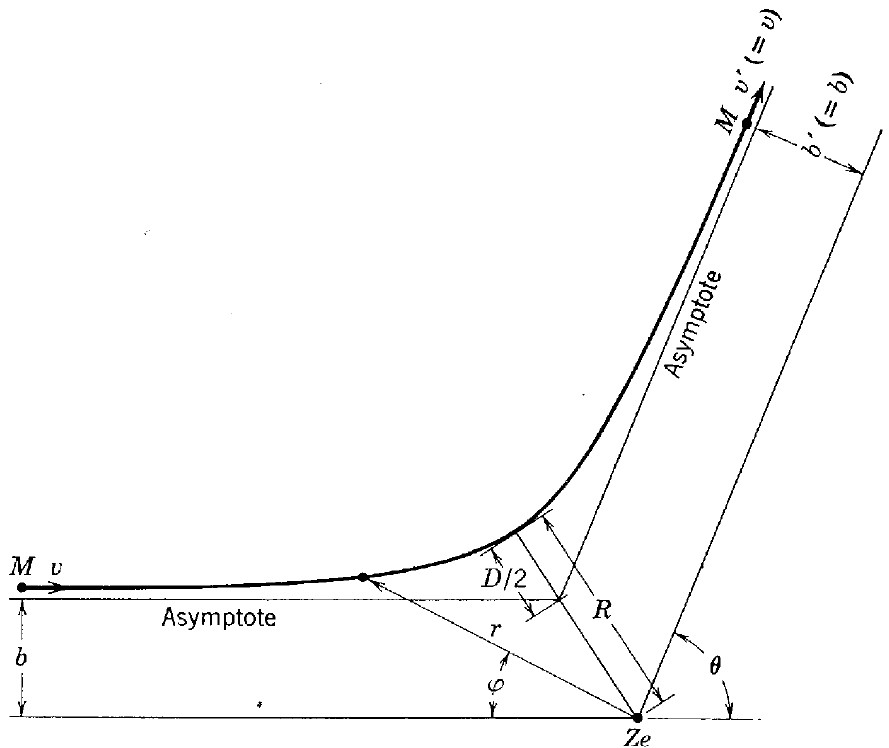
\includegraphics[width=200pt]{fig1_01}
\caption{Traiettoria iperbolica della particella in interazione con un nucleo}
\label{fig:1.1}
\end{figure}
In figura ~\ref{fig:1.1} viene mostrato il modello dello scattering di una particella $\alpha$ di massa M e carica +ze, passante vicino ad un nucleo di carica +Ze.
Il nucleo è fissato al centro del sistema di coordinate.
Prima e dopo la collisione la particella avrà una traiettoria rettilinea (prima con velocità v poi con velocità v') in quanto la forza coulombiana è trascurabile dopo una certa distanza .
Per determinare la posizione della particella si sfruttano le coordinate polari $r(t), \varphi$. 
La distanza tra la traiettoria della particella e la linea parallela passante per il nucleo (asse orizzontale del sistema) è definita come il \emph{parametro d'impatto} $b$.
L'angolo di scattering $\theta$ è dato dall'intersezione dell'asse orizzontale con la parallela alla traiettoria finale passante per il nucleo.

Siccome il nucleo viene considerato fisso, l'energia cinetica finale della particella deve essere identica a quella iniziale. 
Velocità e parametro d'impatto sono costanti prima e dopo l'impatto a causa della conservazione dell'energia cinetica e del momento angolare.
\begin{equation}
Mvb=Mv'b'=L \hspace{1cm} \frac{1}{2}Mv^2=\frac{1}{2}Mv'^2
\end{equation}
\emph{si ha la conservazione del momento angolare perché in presenza di una forza centrale}
\[
dL/dt=\bar r \times \bar F (r)=0
\]
\emph{si ha quindi che raggio e forza sono sempre paralleli}.

Sfruttando nuovamente il momento angolare si cerca ora di ottenere il differenziale del tempo
\begin{equation}
|L|=|\bar r \times m\bar v|=mvb=mv_\perp r=m\omega r^2=m\frac{d\varphi}{dt}r^2
\end{equation}
dove la velocità tangenziale è $v_\perp=\omega r$ e $\omega=d\varphi/dt$ è la velocità angolare. 
Si ottiene quindi
\begin{equation}
\frac{d\varphi}{dt}=\frac{vb}{r^2}\hspace{0.2cm}\to\hspace{0.2cm} dt=d\varphi \frac{r^2}{vb}
\end{equation}
Si può poi introdurre l'interazione elettromagnetica. 
Viene in questo caso sfruttato il teorema dell'impulso
\begin{equation}
\Delta p=\int F_n dt\hspace{1cm}F_n=F\cos\varphi
\end{equation}
dove F è la forza coulombiana tra due particelle
\begin{equation}
F=\frac{1}{4\pi\varepsilon_0}\frac{zZe^2}{r^2}
\end{equation}
La differenza di potenziale risulta essere
\begin{equation}
\Delta p=\int_{-\infty}^{+\infty} \frac{1}{4\pi\varepsilon_0}\frac{zZe^2}{r^2}\cos\varphi dt
\end{equation}
Possiamo quindi sostituire la formula per $dt$ trovata sopra all'interno dell'integrale appena ricavato prestando ovviamente attenzione agli estremi d'integrazione 
\begin{equation}
\begin{split}
t\to -\infty\hspace{2cm}\varphi\to-\frac{1}{2}(\pi-\theta)\\
t\to +\infty\hspace{2cm}\varphi\to+\frac{1}{2}(\pi-\theta)
\end{split}
\end{equation}
\begin{equation}
\Delta p=\int _{-\frac{1}{2}(\pi-\theta)}^{+\frac{1}{2}(\pi-\theta)}\frac{1}{4\pi\varepsilon_0}\frac{zZe^2}{vb}\cos\varphi d\varphi
\end{equation}
Portando fuori dall'integrale tutte le costanti in una constante $A$ si ottiene
\begin{equation}
\Delta p=A[\sin\varphi] _{-\frac{1}{2}(\pi-\theta)}^{+\frac{1}{2}(\pi-\theta)}=A\biggl[\sin\left(\frac{\pi}{2}-\frac{\theta}{2}\right)-\sin\left(\frac{\pi}{2}+\frac{\theta}{2}\right)\biggl]=2A\cos\frac{\theta}{2}
\end{equation}
A questo punto è necessario ricavare la variazione della quantità di moto proiettata sulla normale
\begin{equation}
p_f-p_i=2mv\sin\frac{\theta}{2}
\end{equation}
unendo le due formule per la variazione di quantità di moto si ottiene
\begin{equation}
\begin{split}
2mv\sin\frac{\theta}{2}=2A\cos\frac{\theta}{2} \hspace{0.2cm} & \to \hspace{0.2cm} 2mv\sin\frac{\theta}{2}=\frac{zZe^2}{4\pi \varepsilon_0vb}\cos\frac{\theta}{2}\\
\tan\frac{\theta}{2}=\frac{zZe^2}{4\pi\varepsilon_0mv^2}\frac{1}{b} \hspace{0.2cm} & \to\hspace{0.2cm} \tan\frac{\theta}{2}=K\frac{1}{b}
\end{split}
\end{equation}
$K$ è semplicemente una costante che include tutte le costanti del moto.
Da quest'ultima formula si può vedere che se $b\to 0$ ovvero nel caso di un urto frontale si otterrà come angolo $\theta=\pi$ e quindi la particella sarà rispedita alla sorgente.

\paragraph{Sezione d'urto differenziale}

Si procede ora a ricavare la sezione d'urto differenziale, ovvero lil rapporto differenziale tra le particelle incidenti e quelle scatterate per un certo angolo solido e parametro d'impatto. 
\begin{figure}[h]
\centering
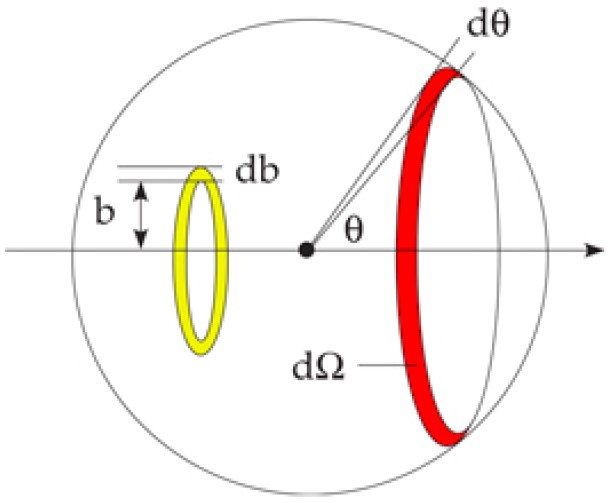
\includegraphics[width=150pt]{fig1_02}
\caption{Schematizzazione della sezione d'urto differenziale in base al parametro d'impatto e all'angolo solido.}
\label{fig:1.2}
\end{figure}

L'area delle particelle incidenti è data dalla formula 
\begin{equation}
d\sigma=2\pi b |db|
\end{equation}
Le particelle definite in quest'area saranno diffuse all'angolo 
\begin{equation}
d\Omega =2\pi \sin\theta d\theta
\end{equation}
Facendo il rapporto tra le due aree si ottiene la sezione d'urto differenziale dal punto di vista cinematico
\begin{equation}
\frac{d\sigma}{d\Omega}=\frac{b(\theta)}{\sin\theta}\frac{db}{d\theta}
\end{equation}

Si può a questo punto unire le formule ricavando $b$ rispetto a $\theta$ 
\begin{equation}
\frac{db}{d\theta}=\frac{d}{d\theta}\biggl|\frac{k}{\tan\frac{\theta}{2}}\biggl|=\frac{K}{\tan^2 \frac{\theta}{2}}\frac{1}{2}\frac{1}{\cos^2\frac{\theta}{2}}
\end{equation}
\begin{equation}
\begin{split}
\frac{d\sigma}{d\Omega}&=\frac{1}{2}\frac{K^2}{\tan^3 \frac{\theta}{2}}\frac{1}{\cos^2\frac{\theta}{2}\sin^2\frac{\theta}{2}}=\frac{K^2}{4\sin^4\frac{\theta}{2}}\\
&=\frac{1}{16}\left(\frac{zZe^2}{4\pi\varepsilon_0 T}\right)\frac{1}{\sin^4\frac{\theta}{2}}
\end{split}
\end{equation}
Introduciamo ora un po' di costanti che aiutano a semplificare questa formula e spesso usate in fisica subatomica
\begin{equation}
\alpha=\frac{b^2}{4\pi\varepsilon_0\hbar c}=\frac{1}{137}\hspace{1cm}\hbar c=197 MeV\cdot fm
\end{equation}
$\alpha$ è denominata \emph{costante di struttura fine}. 

La formula con queste costanti diventa
\begin{equation}
\frac{d\sigma}{d\Omega}=\frac{z^2Z^2}{16}\alpha^2\left(\frac{\hbar c}{T}\right)^2 \frac{1}{\sin^4\frac{\theta}{2}}
\end{equation}
La cosa straordinaria di questa sezione d'urto sta nel fatto che, per delle coincidenze sotto un certo punto di vista fortuite, è uguale a quella calcolata con la meccanica quantistica. Questo succede perché nell'interazione di particelle alfa con il nucleo gli spin sono ininfluenti. 

Commenti alla sezione d'urto:
\begin{itemize}
\item La sezione d'urto diminuisce all'aumentare dell'energia cinetica (inversamente proporzionale a $T^2$).
\item Decresce rapidamente all'aumentare di $\theta$.
\item \'E proporzionale al quadrato delle cariche.
\end{itemize}


%%Nuova subsection--------------------------------------------------
\subsection{Sezione d'Urto Quantistica (Regola d'Oro di Fermi)}
Il cambiamento essenziale che avviene in meccanica quantistica riguarda la probabilità d'interazione. Infatti se nella trattazione classica la probabilità derivava da una serie di considerazioni classiche, nella trattazione quantistica deriva dalla \emph{regola d'oro di Fermi} definita come
\begin{equation}
P=\frac{2\pi}{\hbar}|H_{f,i}|^2\rho(E_f)
\end{equation}
I contributi che compongono questa probabilità d'interazione sono:
\begin{itemize}
\item $H_{f,i}$ è l'elemento dell'Hamiltoniana della perturbazione, ovvero la probabilità che la sezione d'onda iniziale passi alla sezione d'onda finale.
\begin{equation}
H_{f,i}=<f|H|i>=\int \psi*_f(r)H(\bar r)\psi_i d^3r
\end{equation}
(\emph{La probabilità di passaggio di uno stato iniziale ad uno stato finale si valuta effettuando questo integrale tra lo stato iniziale e quello finale della Hamiltoniana di perturbazione}).

Le funzioni d'onda sono quelle che descrivono le nostre particelle $\alpha$
\begin{equation}
H(r)=V(r)=\frac{zZe^2}{4\pi \varepsilon_0r}
\end{equation}
Quali sono quindi gli stati (funzioni d'onda) che descrivono gli alfa?

Ad una certa distanza iniziale saranno onde piane
\begin{equation}
\psi_i \sim e^{ikr} \hspace{1cm}\bar p=\hbar\bar k\hspace{0.5cm}\bar k=\frac{\bar p}{\hbar}
\end{equation}
Dopo l'interazione, ovvero quando le particelle non subiranno più il potenziale coulombiano, si avrà che la funzione sarà nuovamente un'onda piana ma con vettore d'onda variato (legato ovviamente alla quantità di moto)
\begin{equation}
\psi_i \sim e^{ik'r}\hspace{1cm} \bar p'=\hbar\bar k'\hspace{0.5cm}\bar k'=\frac{\bar p'}{\hbar}
\end{equation}
Tornando alla regola d'oro di fermi, ciò mi dice che la probabilità d'interazione dipende dalla probabilità che il mio potenziale faccia passare le mie particelle da una certa quantità di moto ad un'altra.

\item L'altro contributo si ha dalla densità degli stati finali $\rho(E_f)$, ovvero il numero di stati finali accessibili al sistema, maggiore è il tipo di capienza nello spazio delle fasi maggiore è la probabilità. Per ora trascureremo questo contributo per trattarlo più avanti.
\end{itemize}

Studiamo quindi la variabilità della probabilità in base alle funzioni d'onda. 
Si ha
\begin{equation}
H_{f,i}\simeq \int e^{-ik'r} V(r)e^{+ikr}=\int V(r)e^{-i(k'-k)r}
\end{equation}
La variazione dell'impulso in questa trattazione diventa  
\begin{equation}
\begin{split}
\bar p &=\hbar \bar k\\
\bar p &=\hbar k'\\ 
\Delta p =\bar p' -\bar p&=\bar q=\hbar (k'-k)
\end{split}
\end{equation}
Sostituendo nella formula dell'Hamiltoniana si trova
\begin{equation}
\begin{split}
H_{f,i}&=\int V(r) e^{-i\frac{\bar q}{\hbar}r}d^3r\\
&=\frac{zZe^2}{4\pi\varepsilon_0}\int \frac{1}{r}e^{-i\frac{\bar q}{\hbar}r}
\end{split}
\end{equation}
Come si può vedere questa formula corrisponde ad una trasformata di Fourier, e quindi risulta facile risalire alla funzione d'origine. Ciò che si ottiene alla fine è
\begin{equation}
H_{f,i}=\frac{zZe^2}{4\pi\varepsilon_0}\frac{4\pi\hbar^2}{q^2}
\end{equation}
l'ultima frazione è la parte che si utilizza per calcolare la sezione d'urto differenziale
\begin{equation}
\frac{d\sigma}{d\Omega}\propto P\simeq |H_{f,i}|^2\sim\frac{1}{q^4}
\end{equation}
Si può vedere che questa funzione, ricavata quantisticamente, esprime una dipendenza dipendenza proporzionale a $1/q^4$, che corrisponde al momento trasferito ($\delta p$) alla quarta.
 
Sorge spontaneo chiedersi se questo sia consistente con la formula derivata classicamente. La risposta è affermativa e si può dimostrare. Prendiamo infatti la variazione classica della quantità di moto.

\begin{figure}[h]
\centering
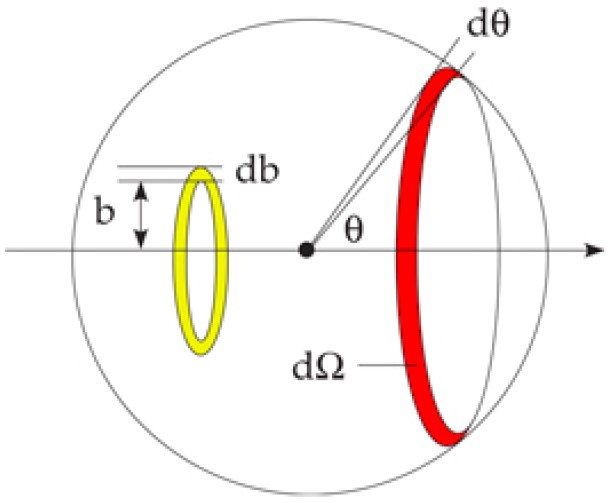
\includegraphics[width=120pt]{fig1_03}
\label{fig:1.3}
\end{figure}

\begin{equation}
\begin{split}
\bar{\Delta p} &=\bar p'-\bar p=q=2p \sin\frac{\theta}{2}\\
q^2 &=4m^2v^2\sin^2 \frac{\theta}{2}
\end{split}
\end{equation}
Ricordando la formula classica dell'energia cinetica
\begin{equation}
T =\frac{1}{2}mv^2
\end{equation}
Si ottiene che 
\begin{equation}
q^2=8mT\sin^2\frac{\theta}{2}
\end{equation}
\'E resa evidente quindi la stessa dipendenza che si aveva nel caso classico, questo è dovuto a vari fattori, ma quello principale è che ci troviamo ad energie non relativistiche.
Altre supposizioni fatte nella trattazione classica erano che le particelle non avessero interazioni di spin, abbiamo trascurato inoltre che i nuclei avessero rinculo. 
Queste sono tutte assunzioni buone ma che per risultati più precisi rilasceremo in trattazioni più avanzate.

\paragraph{Raggio nucleare} Quello che ci si domanda ora è il motivo per cui considerando solamente l'interazione coulombiana si riescano ad ottenere risultati così buoni.

Si consideri il raggio nucleare stimato de Rutherford per la sua trattazione tramite scattering $\alpha$. 
Si cerchi la distanza di massimo avvicinamento della particella a nucleo, che si otterrà per un'energia pari a 
\begin{equation}
V=K_\alpha \hspace{0.5cm}\to \hspace{0.5cm}K_{\alpha}=\frac{1}{4\pi\varepsilon_0}\frac{zZe^2}{R_0}
\end{equation}
Invertendo la formula si ricava il raggio di Rutherford
\begin{equation}
\begin{split}
R_0 &=\frac{1}{4\pi\varepsilon_0}\frac{zZe^2}{K_{\alpha}}\frac{\hbar c}{\hbar c}\\
&\simeq\frac{1}{137}\frac{2\cdot 79}{4\cdot 9 MeV}\hbar c\\
&=46 fm
\end{split}
\end{equation}

Questa è una sovrastima del raggio nucleare in quanto si sa attualmente che il raggio corrisponde ad 8 fermi. 
Questo errore è dovuto al fatto che non vi è interazione nucleare nello scattering di Rutherford ma semplicemente elettrostatica, il che spiega anche la perfetta corrispondenza dei suoi dati con la trattazione teorica.

Supponiamo quindi di riuscire ad aumentare l'energia delle particelle $\alpha$ (quello che accade negli acceleratori). 
Si supponga poi di utilizzare come target del piombo e di porre un rivelatore a $60^o$. 
\begin{figure}[h]
\centering
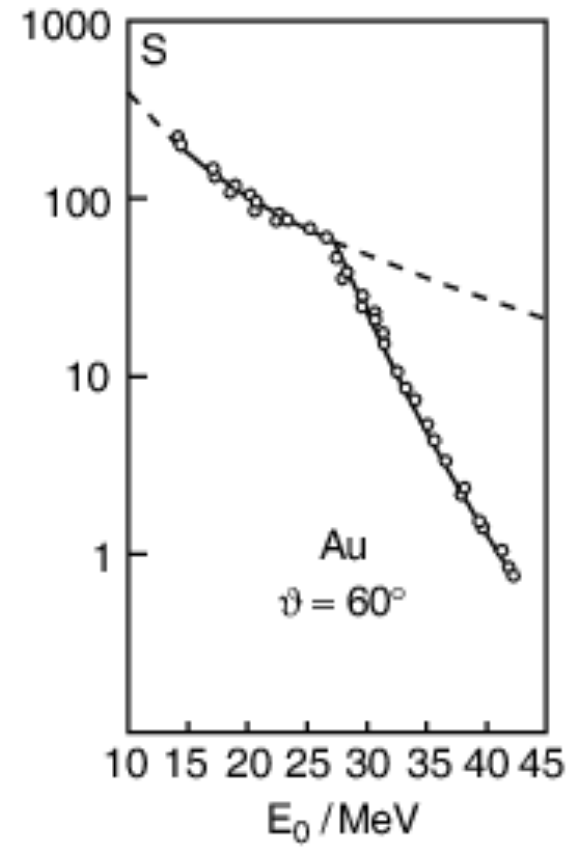
\includegraphics[width=120pt]{fig1_05}
\caption{Esperimento di Rutherford su target di piombo in confronto al risultato calassico}
\end{figure}
Si può osservare che l'andamento del numero di particelle scatterate per energie inferiori a 27,5 MeV rispecchia esattamente l'andamento di Rutherford ma poi ha un cambio drastico. 
Questo accade perché oltre un certo raggio subentra l'interazione per forza forte
\begin{equation}
R=\frac{Q_1Q_2}{4\pi\varepsilon_0KE}=8.59 fm
\end{equation}
La sovrastima di Rutherford era dovuta al fatto che le particelle da lui usate avevano effettivamente interazione puramente coulombiana.


%%Nuova subsection-----------------------------------------------------
\subsection{Derivazione con l'Elettrodinamica Quantistica}
Questa trattazione è possibile in modo semplice grazie ai diagrammi di Feynman che semplificano il tecnicismo della fisica teorica rendendola accessibile ai fisici sperimentali.
\begin{figure}[h]
\centering
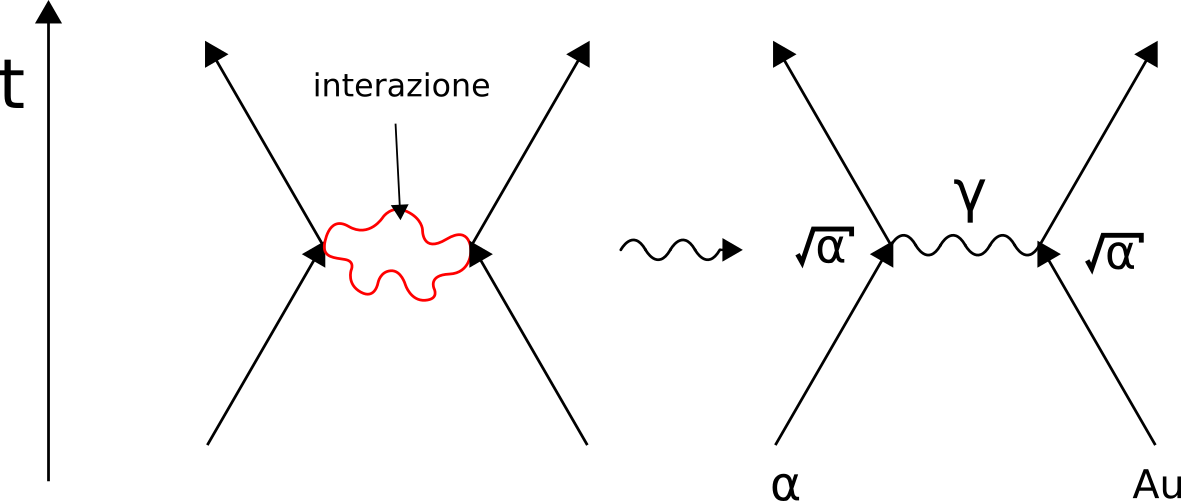
\includegraphics[width=300pt]{fig1_04}
\caption{Diagrammmi di Feynman}
\end{figure}
Secondo i diagrammi di Feynman ogni particella reale è descritta da una linea continua. Una cosa da tenere sempre presente è la direzione in cui si svolge l'azione temporale, in questo caso si svolge verso l'alto ma è solamente una rappresentazione grafica di un'interazione.
Nelle teorie quantistiche di campo l'interazione viene descritta tramite lo scambio di una particella.
La grande novità che è stata introdotta da queste teorie è che l'interazione non sia descritta tramite un campo ma attraverso lo scambio di particelle virtuali.

Come si ricava quindi la sezione d'urto?

La particella alfa emette un fotone virtuale e questo viene descritto tramite una costante di accoppiamento posta ai vertici (ovvero nel punto d'impatto) denominata $\sqrt{\alpha}$. 
L'interazione viene rappresentata da quello che si chiama propagatore ovvero la linea interna che congiunge i due vertici.
\begin{equation}
\propto \frac{1}{Q^2+M^2C^2}
\end{equation}
dove $Q^2$ è il momento trasferito, $M$ è la massa della particella mediatrice (bosone vettore), $\gamma$ è il fotone.
Come si calcola l'ampiezza della transizione?
\begin{equation}
\begin{split}
|M_{f,i}| &=\sqrt{\alpha}\frac{1}{Q^2}\sqrt{\alpha}=\frac{\alpha}{Q^2}\\
P &\propto |M_{f,i}|^2 =\frac{\alpha^2}{Q^4}
\end{split}
\end{equation}
Dove P è la probabilità di transizione della particella, corrispondente alla sezione d'urto.
Si può notare anche qui che la proporzionalità trovata per le altre trattazione è mantenuta.




%Zarantonello Umberto 20/04/21

\section{Il Nucleo}
La secoda particella ad essere rivelata dopo l'elettrone fu il protone. 
La prima evidenza sperimentale è dovuta a Rutherford nel 1917 sfruttando sempre le particelle alfa, questa volta in collisione con l'aria dove è presente l'azoto N 
\begin{equation}
^4_2He +^{14}_{7}N_{7}\longrightarrow ^{17}_8O_9+protone
\end{equation}
Al tempo uno dei modelli nucleari era che il nucleo fosse composto da un certo numero $A$ di protoni ed un numero $A-Z$ di elettroni (con Z il numero di elettroni della nuvola elettronica) in modo da bilanciare la carica dei protoni rendendo l'atomo stabile.
Analizziamo dunque la possibilità di avere un nucleo di questo tipo.
Che potenziale elettroagnetico dovrebbero gestire i protoni?
\[E=\frac{Ze^2}{4\pi\varepsilon_0R}\]
dove $R=R_0 A^{1/3}=1.2fm\cdot A^{1/3}$ (formula empirica per il calcolo del raggio nucleare). 
Calcolando si ottiene quindi
\[E=-1.20\frac{Z}{A^{1/3}MeV}\]
Per esempio, ponendo A=140 e Z=58 l'energia cinetica che si ottiene è $E=-13.4MeV$ (elettrone con energia relativistica quindi $E=pc$). Un elettrone con tale energia cinetica è possibile che resti confinato all'interno del nucleo?
\[\lambda=\frac{h}{p}=2\pi \frac{\hbar c}{pc}=\frac{2\cdot 3.14\cdot 200MeV\cdot fm}{13.4MeV}\simeq 90fm\]
L'elettrone non può essere quindi confinato nel nucleo perchè la sua lunghezza d'onda è molto maggiore.

\paragraph{La scoperta del Neutrone} fu fatta da Chadwick che fu il primo ad intuire, da un'esperienza che in realtà era già stata fatta da più fisici, la presenza di un'altra particella. 
La situazione che si verificava era che tramite l'emissione di particelle alfa generate dal polonio, fatte collidere su un target di Berilio, si otteneva una radiazione che riusciva ad attraversare uno schermo spesso di piombo, il che suggeriva il fatto che fosse una radiazione neutra (impossibile per della radiazione carica attraversare uno schermo troppo spesso). 
Al tempo l'unica radiazione neutra conosciuta era la radiazione elettromagnetica il che fece pensare ad una reazione cle tipo
\[
^9_4Be+^4_2He\longrightarrow[^{13}_6C*]\longrightarrow^{13}_6C+\gamma
\]
Con uno stato intermedio dato da uno stato eccitato del carbonio 13.
Un ulteriore passaggio fu quello di aggiungere dopo lo schermo di Piombo $Pb$ una lastra di paraffina da cui, dopo l'interazione con la radiazione, emergevano protoni con energia pari a $E=7,5MeV$. 
La radiazione gamma doveva quindi possedere un'energia in grado di podurre dei protoni di energia 7,5MeV trammite scattering Compton il che riconduce ad un'energia minima di 55MeV.
Quando il Berilio assorbiva le particelle alfa quest'ultime si trovavano ad un energia di 5MeV, essendo poi una reazione esotermica si aveva che il Q della reazione corrispondeva a $Q=10MeV$, il che riconduceva ad un energia massima disponibile di 14MeV.
L'unica spiegazione possibile era che si trattava quindi di una particella nuova, neutra e con la stessa massa del protone.


%Zarantonello Umberto 2021-05-08

\section{Modelli Nucleari}
I modelli nucleari sono un tipo di supporto teorico che ci permette di interpretare le proprietà legate prima ai processi di decadimento e poi a quelli di fissione e fusione nucleare.
Come vedremo i modelli nucleari sono molto eterogenei e partono da presupposti che possono arrivare a contraddirsi.
Il modello a goccia per dire è opposto al modello di Fermi.
Questo esprime la difficoltà che si ha ad associare le proprietà dei nuclei a principi primi.
Quelli che introduciamo sono modelli fenomenologici o semi empirici, ciò indica che faremo delle supposizioni a partire da dati empirici per spiegare ciò che si vede.
Questo approccio è dovuto proprio alla mancanza di una teoria che con principi elementari esprima le proprietà dei nuclei.

%nuova sezione--------------------------------------------------
\subsection{Formula semi-empirica di massa}
Quello che verrà trattato in questa sezione riguarda quello che tiene legato il nucleo. 
Grazie all'esperimento di Rutherford sappiamo che il nucleo è formato da una carica positiva molto densa concentrata al centro, circondata poi da elettroni.
La cosa sorprendente di questa scoperta fu principalmente legata alla dimensionalità infatti, prima di Rutherford era logico pensare che la materia fosse densa, ma quello che ci rivelano i dati è appunto che tra il raggio nucleare e il raggio atomico c'è un fattore $10000$ che rende la materia di fatto "spazio vuoto".

\'E stato visto poi, con gli esperimenti di Rutherford e Chadwick, che il nucleo è composto da protoni e neutroni, in particolare con il nucleo può essere esplicitato con la formula
\begin{equation}
^{A}_{Z}X_{N}
\end{equation}
dove $X$ indica l'elemento, $A$ è il numero di massa, ovvero la somma di neutroni e protoni, $Z$ è il numero atomico, ovvero il numero di protoni e infine $N$ è il numero di neutroni ($A=Z+N$).
Si sa inoltre che la carica dell'atomo è assolutamente neutra e quindi che il numero di protoni è esattamente uguale al numero di elettroni.

\begin{figure}[h]
\centering
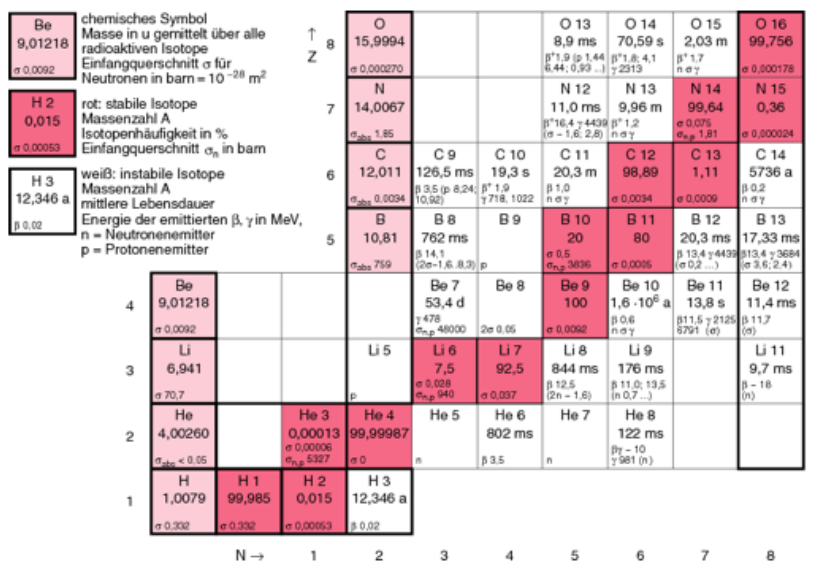
\includegraphics[width=300pt]{fig5_01}
\caption{Tavola dei Nuclidi}
\label{fig:5_01}
\end{figure}
La tavola dei nuclidi è uno strumento utile in fisica subatomica.
Sulla diagonale è rappresentata la linea degli elementi che possiedono un numero equivalente di neutroni e protoni.
Per numero di protoni bassi, i nuclidi che si trovano in natura, ovvero i nuclidi stabili, si trovano proprio lungo questa diagonale. 
Aumentando però il numero atomico i nuclidi stabili diventano quelli con un numero sempre maggiore di neutroni rispetto ai protoni.
Intorno a questa zona di nuclidi stabili vi è poi una zona di nuclidi instabili.
Oltre questa zona non vi sono poi più nuclidi, ne stabili ne instabili.

Cosa vuol dire atomo instabile?

Per nuclidi con protoni in eccesso, rispetto ai nuclidi stabili, ciò che accade è che l'atomo tende a decadere, ovvero uno o più protoni in eccesso subirà la reazione di decadimento $\beta^+$
\begin{equation}
p\longrightarrow n+e^+\nu_e
\end{equation}
Nei nuclidi che hanno esuberanza di neutroni, la reazione che avverrà riguarda i neutroni e si definisce decadimento $\beta^-$
\begin{equation}
n\longrightarrow p+e^- +\bar{\nu_e}
\end{equation}
(nelle formule sopra $p$ indica il protone, $n$ il neutrone, $e^-, e^+$ rispettivamente l'elettrone e il positrone, $\nu_e, \bar{\nu_e} $ il neutrino e l'antineutrino elettronici).

In questo tipo di trasformazioni si ha che la carica e il numero leptonico si conservano sempre. 
La carica è abbastanza evidente, per quanto riguarda il numero leptonico per ora ci basta sapere che viene conservato.

Com'è intuibile nel decadimento $\beta$ il nucleo si trasmuta variando il tipo di nucleo, solo che nel primo caso si ottiene un nuclide con un protone in meno dell'originale mentre nel secondo caso il nuclide avrà il numero dei protoni aumentato.
\begin{equation}
\begin{split}
\beta^+\hspace{0.5cm}^A_ZX \longrightarrow ^A_{Z-1}Y+e^+ +\nu_e\\
\beta^-\hspace{0.5cm} ^A_ZX \longrightarrow ^A_{Z+1}Y+e^- +\bar{\nu_e}
\end{split}
\end{equation}
Nella tavola dei nuclidi si avrà quindi che le reazioni provocheranno uno spostamento dell'elemento all'interno della tavola in diagonale (perpendicolarmente alla bisettrice del grafico).

Introduciamo ora il concetto di \emph{energia di legame}. 
Se supponiamo che all'interno di un nucleo ci siano Z protoni e N neutroni, prendendo la massa delle particelle libere che compongono il nucleo e confrontandola con la massa delle stesse particelle legate nel nucleo, si ottiene che quest'ultima è sempre minore della somma delle masse delle particelle libere.
Si ha quindi che parte della massa si trasforma in energia di legame, secondo la formula 
\begin{equation}
\Delta m c^2 \to BE
\end{equation}
La massa che va a formare il legame, chiamata massa mancante, è proprio la responsabile della diminuzione di massa nelle particelle legate rispetto alle particelle libere.

Calcoliamo ora per esempio l'energia che si ottiene trasformando un protone
\begin{equation}
p=10^{-27}kg\hspace{1cm} m_pc^2= 10^{-27}\cdot 9\times10^{16}\cdot 1,6\times10^{-19}\simeq 10^9 eV
\end{equation}

Qual è la differenza quindi tra massa legata e massa libera?
Per un atomo la massa costituente degli elementi degli atomi è
\begin{equation}
(Zm_p+Nm_n+Zm_e)c^2=m_{At}(^A_ZX)c^2+BE_{nuc}+BE_{at}
\end{equation}
dove $BE_{nuc}+BE_{at}$ corrispondono all'energia di legame nucleare e all'energia di legame atomica.
Si possono fare dei calcoli sulla formula sopra
\begin{equation}
Z(m_p+m_e)c^2+Nm_nc^2+Nm_nc^2=m_{At}(^A_ZX)c^2+BE_{nuc}+BE_{at}
\end{equation}
Siccome stiamo ragionando "sperimentalmente" per trovare un modo di calcolare la massa dei nuclei, noi conosciamo già l'energia di legame dell'atomo di idrogeno, per cui
\begin{equation}
m_{At}(^1_1H)c^2+B_{at}^H=m_p+m_e
\end{equation}
che sostituito porta a 
\begin{equation}
Z({m_{At}^1} {_1H c^4})+ZBE^H_{At}+Nm_nc^2=m_{At}(^A_ZX)c^2+BE_{nuc}+BE_{at}
\end{equation}
A questo punto posso notare che l'energia di legame dell'atomo di idrogeno e l'energia di legame dell'atomo si possono semplificare, ottenendo così l'energia di legame
\begin{equation}
BE_{nuc}=Z(m_{At}^1{_1Hc^4})+Nm_nc^2-m_{At}(^A_ZX)c^2
\end{equation}
Posso quindi misurare semplicemente l'energia di legame, infatti la massa dell'idrogeno è nota così come la massa del neutrone; basterà semplicemente misurare la massa dell'atomo legato.

\paragraph{Qual è la natura della forze che tengono insieme un nucleo?}
\'E chiaro che all'interno del nucleo ci debba essere una forza molto grande perché questo possa esistere, si deve infatti controbilanciare la forza elettrostatica di repulsione tra cariche uguali. 
Essendo che in natura esistono nuclei con numero atomico fino a 100 questa forza deve essere  almeno un fattore 100 rispetto alla forza elettrostatica.
Il modello che cerca di spiegare questa forza è appunto il \emph{modello a goccia}.

Ipotizziamo di avere una forza che agisce tra tutte le coppie di nucleoni, questo vuol dire che questa forza non distinguerà tra protoni e neutroni.
Siccome tra ogni coppi ci dovrà essere una forza procediamo a costruire il modello.
Tra tre particelle il numero di coppie possibili è 3, tra quattro particelle si formeranno 6 coppie. 
Si può quindi evidenziare una legge che stabilisce il numero di coppie in un nucleo con numero di massa $A$
\begin{equation}
\frac{A(A-1)}{2}=\frac{A^2-A}{2}
\end{equation}
Questo vuol dire che l'energia di legame totale del nucleo sarà proporzionale a $A^2$ e l'energia di ogni legame singolo sarà proporzionale a $A$.
\begin{equation}
BE\propto A^2\to \frac{BE}{A}\propto A
\end{equation}
Abbiamo quindi creato un'ipotesi che ora va verificata.
Se quest'ipotesi fosse vera si avrebbe che $BE/A$ e $A$ devono risultare proporzionali e aumentare linearmente l'uno rispetto all'altro.
I dati sperimentali ci dicono in realtà che l'energia di legame aumenta quasi linearmente fino ad un massimo (coincidente con il ferro $^{56}Fe$) e che dopo si stabilizza ad un valore $\sim 8MeV$ rimanendo circa costante all'aumentare di A.
\begin{figure}[h]
\centering
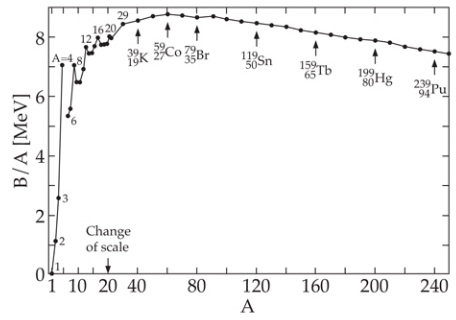
\includegraphics[width=180pt]{fig5_04}
\caption{Grafico sperimentale  dell'energia di legame in funzione con l'aumento del numero di massa}
\end{figure}

Questo errore deriva dal fatto che abbiamo supposto che i nucleoni interagiscano infinitamente anche con i nucleoni più distanti, questo è stato dimostrato non essere vero e anzi che si raggiunge una saturazione.

Si ha quindi che due nucleoni lontani non si parlano.
La forza nucleare è dunque una forza a corto range.

Abbiamo imparato che l'energia di legame (\emph{Bending energy}) corrisponde a 
\begin{equation}
BE=a_vA
\end{equation}
dove $a_v$ è un termine di volume.

Questa formula avrà intuitivamente una serie di termini correttivi. 
Una prima correzione è dovuta al fatto che sicuramente i nucleoni centrali avranno più legami rispetto ai nucleoni sulla superficie della sfera (da qui deriva il nome di modello a goccia, infatti si basa sulla stessa struttura delle gocce di acqua).
Continuando ad approssimare devo tener conto di un termine di superficie che diminuisce l'energia di legame.
\begin{equation}
BE=a_vA-a_sA^{2/3}
\end{equation}
$A^{2/3}$ esprime la dipendenza dalla superficie perché il raggio nucleare ha formula
\[
R=R_0A^{1/3}
\]
e la superficie della sfera è
\[
S=4\pi R^2
\]
il che restituisce una proporzionalità di superficie di $A^{2/3}$.

Il terzo termine deriva dal fatto che all'interno del nucleo sono presenti i protoni che possiedono una forza di repulsione elettrostatica tra loro
\[
F_Q=\frac{Q_1Q_2}{4\pi \varepsilon_0 R^2}
\]
In realtà ciò che interessa a noi è l'energia potenziale.
\[
PE\propto \frac{1}{R}=\frac{K}{A^{1/3}}
\]
Il termine coulombiano della forza di legame è quindi
\begin{equation}
=a_c\frac{Z(Z-1)}{A^{1/3}}
\end{equation}
Aggiungendo questo termine si trova che l'energia di legame è
\begin{equation}
BE=a_vA-a_sA^{2/3}-a_c\frac{Z(Z-1)}{A^{1/3}}
\end{equation}

Perché la formula dell'energia di legame sia completa mancano altri due termini.
Mentre tutti i termini trovati fino ad ora si possono considerare come termini classici gli ultimi sono termini puramente quantistici. 

Il primo è legato al fatto che i protoni e i neutroni possono essere descritti come intrappolati in una buca di potenziale.
All'interno di una buca di potenziale i livelli sono quantizzati e soprattutto equispaziati.
Supponiamo che esistano due buche di potenziale, una dei protni e una dei neutroni, all'interno di questa buca i nucleoni si dispongono con spin antiparallelo.
Continuando ad aggiungere neutroni nella buca e superando il numero di protoni io avrò che mi ci vuole meno energia per estrarre un neutrone, in quanto avranno occupato dei livelli energetici più alti dei protoni (sono meno fortemente legati).
Questo eccesso di energia corrisponde a 
\begin{equation}
E= 2S+ 2(2S)+2(3S)+ ...+ 2(\frac{X}{2}S)
\end{equation}
dove $S$ è la differenza energetica tra i livelli che viene moltiplicato per il numero di livelli in eccesso, $X$ è infatti l'eccesso di neutroni ovvero $X=N-Z$.
Quella sopra è evidentemente una serie geometrica che da come somma
\begin{equation}
E=2S\biggl[\frac{X}{2}\biggl(\frac{X}{2}+1\biggl]/2=S\biggl(\frac{X^2}{4}+\frac{X}{2}\biggl)
\end{equation}
Se X è grande portò ignorare il termine $X/2$.
Se $A$ aumenta ciò che succede è che non  aumento il livello massimo occupato all'interno della buca ma diminuisce la spaziatura tra i livelli stessi
\begin{equation}
A\uparrow \rightarrow S\downarrow \rightarrow S\propto \frac{1}{A}
\end{equation}
Quindi 
\begin{equation}
S\frac{X^2}{4}\propto \frac{1}{A}(N-Z)^2
\end{equation}
Il termine che si andrà ad aggiungere alla formula di legame nucleare definito anche termine di simmetria sarà
\begin{equation}
a_{sym}\frac{(N-Z)^2}{A}
\end{equation}
La formula aggiornata sarà ora
\begin{equation}
BE=a_vA-a_sA^{2/3}-a_c\frac{Z(Z-1)}{A^{1/3}}-a_{sym}\frac{(N-Z)^2}{A}
\end{equation} 

L'ultimo termine che manca è legato al fatto che i nucleoni tendono ad accoppiarsi con spin antiparallelo e quindi risulta che i nuclei con numero di nucleoni pari saranno più legati rispetto a quelli con numero negativo.
Nella tabella sono raffigurati i valori che può assumere l'ultimo termine di correzione in base al numero di nucleoni che sono presenti nel materiale.
\begin{figure}[h]
\centering
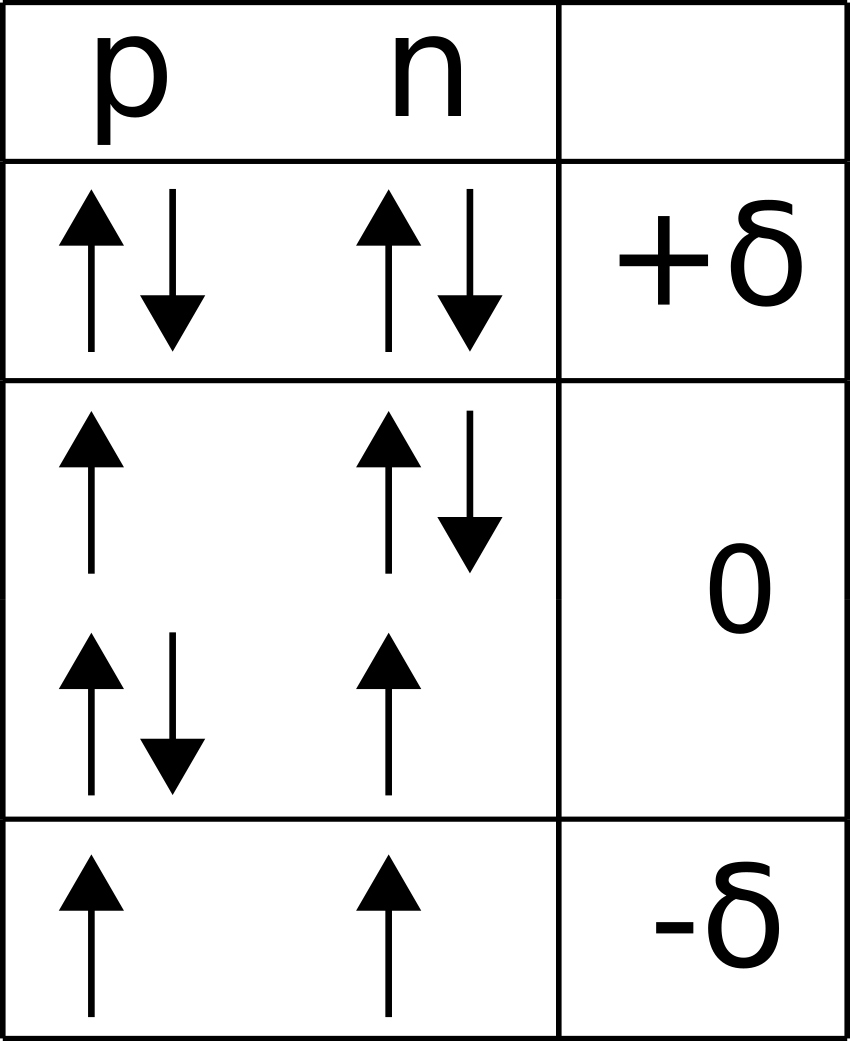
\includegraphics[width=120pt]{fig5_02}
\end{figure}

La formula finale ottenuta è quindi
\begin{equation}
BE=a_vA-a_sA^{2/3}-a_c\frac{Z(Z-1)}{A^{1/3}}-a_{sym}\frac{(N-Z)^2}{A}+\delta
\end{equation}

Ora possiamo finalmente calcolare la massa del la massa del nucleo
\begin{equation}
\begin{split}
m_{nucl} ^A-Z X c^2 &=Z m_p c^2+N m_n c^2- BE_{nucl} \\
&=Zm_pc^2+Nm_nc^2-\biggl[ a_v A-a_s A^{2/3}-a_c \frac{Z(Z-1)}{A^{1/3}}-a_{sym}\frac{(N-Z)^2}{A}+\delta \biggl]
\end{split}
\end{equation}
Questa formula è quella che viene chiamata formula semi-empirica di massa.
\'E una formula empirica in quanto deriva da valori sperimentali ma non lo è totalmente in quanto sono stati inseriti pure vari termini determinati con la teoria.
Ciò che non abbiamo ancora specificato sono i valori dei termini moltiplicativi. 
Questi possono variare in base ai testi o ai fit da cui sono derivati, ogni set di valori possiede numeri consistenti tra loro.
\begin{equation}
\begin{split}
a_v &=15,8MeV\\
a_s&=18,3MeV\\
a_c&=0,714MeV\\
a_{sym}&=23,2MeV\\
\delta=33,5MeV
\end{split}
\end{equation}
\begin{figure}[h]
\centering
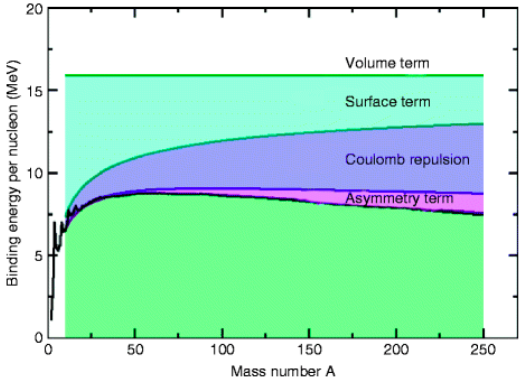
\includegraphics[width=180pt]{fig5_03}
\caption{Modifiche all'energia di legame date da ogni termine}
\end{figure}

\paragraph{Limiti alla creazione dei nuclei}
La domanda a cui risponderemo in questo paragrafo è "perché non posso creare le combinazioni che voglio di portoni e neutroni ma solo alcune sono ammesse?".
La risposta molto semplicemente è che la natura richiede che si minimizzi l'energia di massa.

Prendendo quindi la formula semi-empirica di massa e derivandola rispetto a $Z$ ottengo
\begin{equation}
\frac{dM}{dZ}=m_pc^2-m_nc^2-0-0+a_c\frac{2Z-1}{A^{1/3}}+a_{sym}\frac{[-4A+8Z]}{A}
\end{equation}
Ponendo questo differenziale uguale a zero ottengo la condizione richiesta di minimizzare la massa (siccome la massa di neutrone e protone sono circa uguali i due termini di massa si elidono)
\begin{equation}
Z\left(\frac{2a_c}{A^{1/3}}+\frac{8a_{sym}}{A}\right)=\frac{a_c}{A^{1/3}}+4a_{sym}
\end{equation}
Ciò che cerco di ricavare ora è $Z$ che corrisponde al valore di Z che minimizzi la massa
\begin{equation}
Z=\frac{\frac{a_c}{A^{1/3}}+4a_{sym}}{\frac{2a_c}{A^{1/3}}+\frac{8a_{sym}}{A}}
\end{equation}
Questa formula mi restituisce quindi per ogni $A$ il valore di $Z$ che minimizza la massa.
La formula finale è
\begin{equation}
Z=\frac{A}{2}\biggl[\frac{1}{1+0,008A^{2/3}}\biggl]
\end{equation}
Si deduce che se A è piccolo allora $Z=A/2$ e quindi $N=Z$, mentre se A è grande allora $N>Z$.
Intuitivamente questo serve a bilanciare la repulsione elettrostatica dei nuclei con alto numero di protoni.

Studiamo ora gli andamenti che si possono ottenere dalla formula semi-empirica di massa.
Questa formula si può vedere come un polinomio del tipo
\begin{equation}
M=a+ bZ +cZ^2
\end{equation}
Fissato A, la casistica a questo punto si divide in due, i nuclei che hanno numero di massa dispari e quelli con numero di massa pari.

Il caso più semplice si ha per A dispari.
\begin{figure}[h]
\centering
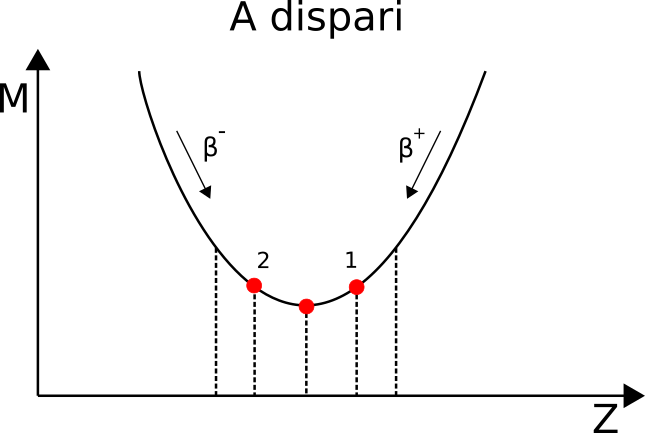
\includegraphics[width=180pt]{fig5_05}
\caption{rappresentazione delle masse possibili al variare di Z con A pari}
\end{figure}
In figura sono rappresentati degli stati possibili con A dispari, lo stato centrale è quello a massa minima e quindi anche quello più stabile.
Procedendo verso lo stato 1 si troveranno i nuclei con un eccesso di protoni mentre al contrario procedendo verso 2 quelli con eccesso di neutroni.
Ciò comporta che 2 avrà la tendenza a decadere nello stato centrale con decadimento  $\beta^-$ mentre 1 decadrà naturalmente con decadimento $\beta^+$.
Nei punti in cui  la parabola assume valori troppo elevati non si ha la presenza di stati.

Nel caso di A pari la faccenda si complica in quanto le parabole possibili sono due, una ad energia più alta e che corrisponde al caso di numero di protoni e neutroni entrambi dispari(Odd-Odd: come già visto sopra questo genera nuclei più instabili) e una a numero di neutroni e protoni pari ad energia più bassa (Even-Even:  quindi con nuclei più stabili).
Si ha quindi la possibilità di avere lo stato centrale o su una parabola o sull'altra portando a due casistiche differenti.
\begin{figure}
\centering
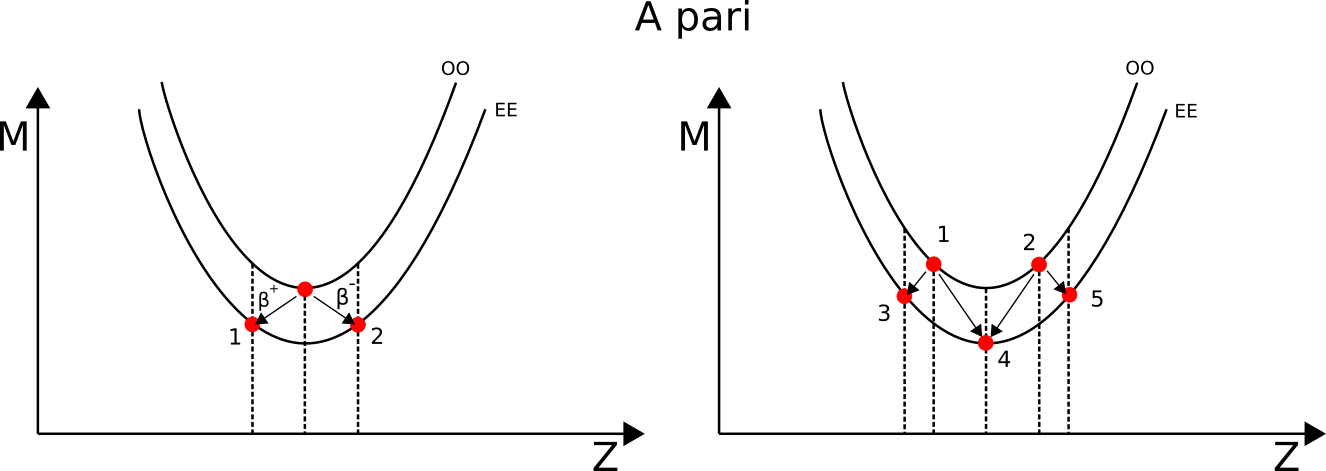
\includegraphics[width=380pt]{fig5_06}
\caption{rappresentazione delle masse possibili al variare di Z con A dispari}
\end{figure}

Nel grafico a sinistra possiamo notare che gli stati stabili sono due in quanto lo stato centrale si trova sulla parabola superiore mentre sulla parabola inferiore sono presenti due stati sullo stesso livello di energia e quindi entrambi con la stessa stabilità. 
Lo stato superiore in questo caso ha due possibilità di decadimento, verso 1 con decadimento $\beta^+$ o verso 2 con decadimento $\beta^-$.
Nel caso per dire che lo stato 1 fosse più elevato di 2, la transizione da 1 a 2 non è impossibile ma altamente improbabile, in quanto pur essendo energeticamente favorevole richiederebbe un secondo decadimento $\beta$ che richiede quindi una seconda probabilità di avvenimento.
Un processo di questo tipo si chiama decadimento \emph{doppio $\beta$}.

Nel grafico a destra è invece mostrato il caso in cui si abbia il nucleo centrale e nella curva più bassa (4), nella curva superiore vi sono invece due nuclei ad energia uguale.
I nuclei 1 e 2 come si vede nel grafico avranno due possibilità di decadimento ciascuno, verso 3,4 e 5.
Come nel caso precedente i decadimento da 3 e 5 verso 4 pur essendo energeticamente favorevoli sono improbabili in quanto decadimenti doppio $\beta$. 
I nuclei 3,4 e 5 sono quindi considerati tutti nuclei stabili.

La zona in cui non si ha la generazione di nuclei, sia provocata da un eccesso di neutroni che di protoni è dovuta al fatto che non è energeticamente favorevole avere nuclei piuttosto che le particelle slegate o un nucleo con numero di massa inferiore e delle particelle libere. 
\begin{equation}
\begin{split}
^A_ZX &\longrightarrow ^{A-1}_ZX+n\\
^A_ZX &\longrightarrow ^{A-1}_{Z-1}Y+p
\end{split}
\end{equation}
Se infatti la somma delle masse slegate a destra delle due reazioni sopra risulta minore della massa dell'atomo legato a sinistra la natura tenderà a dividere il nucleo.
Per lo stesso principio i nuclei che sono troppo pesanti ovvero che possiedono semplicemente troppi nucleoni tenderanno ad emettere particelle $\alpha$; questo tipo di nuclei sono anche quelli che fanno la fissione nucleare ovvero che tenderanno a dividersi in due atomi a numero di massa inferiore.

%nuova sezione--------------------------------------------------
\subsection{Modello di Fermi}
Questo modello a differenza di quello a goccia è un modello a particella singola, ovvero studia l'interazione di una particella con un potenziale generato dalle altre particelle piuttosto che vedere il sistema in generale come insieme di particelle.
Questo perché i sistemi complessi sono difficili da calcolare e inoltre quasi mai si riesce a risolvere i calcoli in maniera analitica.
Il modello di Fermi suppone che il nucleo è composto da due gas di fermioni, protoni e neutroni.
I fermioni sono le particelle che soddisfano alla statistica di Fermi-Dirac, che afferma che due particelle non possono occupare lo stesso stato quantico.
Il risultato di questa ipotesi iniziale sarà poi confermato dal modello.
Trascuriamo l'interazione tra le singole particelle ma le consideriamo confinate in una buca di potenziale che ha delle dimensioni del nucleo.
Questo potenziale è dato dall'interazione media con tutte le altre particelle, quindi in realtà il modello considera le iterazioni ma le approssima ad un potenziale generato proprio da tali  interazioni.
La buca di potenziale che confina i due gas è quindi generata dai gas stessi.
Questa impostazione ci permetterà di fare delle ipotesi sulle proprietà che i nucleoni hanno all'interno del nucleo.
Questo modello fa inoltre parte dei così-detti modelli a particelle indipendenti.

Supponiamo di avere due buche di potenziale, in quanto neutroni e protoni sono considerati particelle indipendenti quindi ognuno avrà la propria buca.
La buca di potenziale dei protoni è meno profonda in quanto questi subiscono anche la repulsione coulombiana, questo ci fa capire un po' di più sul modello a goccia, se ricordiamo infatti si aveva che i nuclei più pesanti possedevano più neutroni a livello di stabilità, proprio a causa di questa repulsione.

Questo modello prevede che sia per i neutroni che per i protoni vi siano dei livelli energetici, occupati fino ad un livello massimo che è il \emph{livello di Fermi}.
Per ogni livello energetico posso sistemare al massimo due particelle con spin opposto,questo per il principio di esclusione di Pauli.

I parametri che caratterizzano questo sistema sono la profondità della buca di potenziale e il livello di Fermi (livello energetico più alto occupato).

Siccome i nucleoni nel nucleo non sono particelle relativistiche possono essere descritti con la meccanica quantistica non relativistica, ovvero quella che viene fatta nella triennale.
Si possono quindi sfruttare le equazioni di Schroedinger.
Vogliamo risolvere l'equazione per una buca di potenziale con energia potenziale
\begin{equation}
\begin{split}
E_{pot} &=V_0\hspace{0.5cm}r\leq a\\
&=0\hspace{0.5cm}r>a
\end{split}
\end{equation}
L'equazione di Schroedinger è indipendente dal tempo e corrisponde a
\begin{equation}
-\frac{\hbar^2}{2m}\frac{d^2}{dr^2}\psi+V_0\psi=E
\end{equation}
La risoluzione è
\begin{equation}
\frac{d^2}{dr^2}\varphi=-\frac{2m}{\hbar}(E-V_0)\varphi
\end{equation}
Per risolverlo bisogna notare che il termine 
\[
-\frac{2m}{h}(E-V_0)>0
\]
Perché $V_0$ è un'energia potenziale di confinamento e una buca di potenziale ha potenziale negativo ($V_0$ è un potenziale attrattivo. 
Quindi posso sostituire il tutto con una variabile reale positiva ottenendo
\begin{equation}
\frac{d^2}{dr^2}\psi+K^2\psi=0 \hspace{0.5cm} K=\sqrt{\frac{2m(E-V_0}{\hbar^2}}
\end{equation}
La soluzione (identica a quella del moto armonico) è
\begin{equation}
\psi=A\sin Kr+B\cos Kr
\end{equation}
A cui devo poi porre le condizioni di annullamento in $0$ e $a$.
\begin{equation}
\begin{split}
&\psi(0)=0\to B=0\hspace{1cm}\psi=A \sin Kr\\
&\psi(a)=0\to Ka=n\pi \to K=n\frac{\pi}{a}\\
&\to E=\frac{p^2}{2m}=\frac{\hbar^2K^2}{2m}=\frac{\hbar^2}{2m}\frac{\pi^2}{a^2}n^2
\end{split}
\end{equation}
Questi sono quindi i livelli energetici consentiti all'interno della buca di potenziale, le funzioni d'onda corrispondenti saranno come in figura.
\begin{figure}[h]
\centering
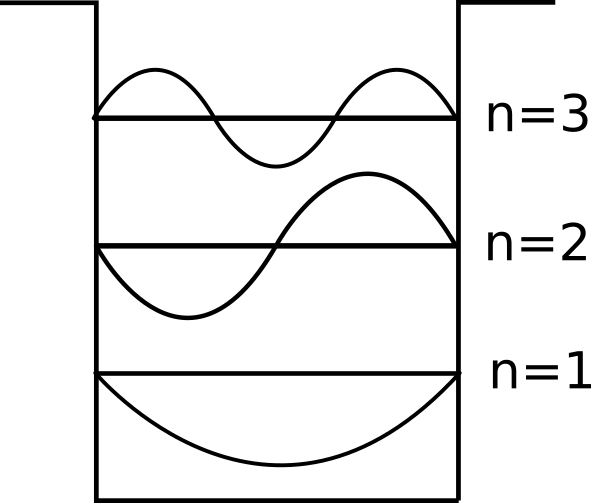
\includegraphics[width=120pt]{fig5_07}
\end{figure}
Se la buca non fosse finita ci sarebbe un'estensione delle funzioni d'onda oltre le pareti della buca.

\paragraph{Stima della profondità della buca di potenziale} Per capire la profondità della buca dobbiamo valutare il numero di stati nucleari nello spazio delle fasi in un volume $V$ e con quantità di moto $p$.
Lo spazio delle fasi è uno spazio a 6 dimensioni che comprende sia le coordinate spaziali che quelle riferite alla quantità di moto nelle tre direzioni. 
Per capire, è un unico spazio a 6 dimensioni che mi dice proprio l'estensione del sistema che sto studiando, quindi qual è lo spazio delle fasi occupato dal gas di neutroni e protoni.
Il numero di nucleoni in funzione di $p$ è dato da
\begin{equation}
dn(p)=\frac{V4\pi p^2 dp}{(2\pi\hbar)^3}
\end{equation}
dove $V$ è il volume nelle coordinate spaziali, $4\pi p^2dp$ è un guscio sferico compreso tra la sfera di raggio $p$ e la sfera $p+dp$, $(2\pi \hbar)^3$ è lo spazio delle fasi occupato da ognuno degli stati quantici, in pratica è un volume di dimensione $\hbar$, quest'ultima quantità è legata al principio d'indeterminazione $\Delta p\Delta x \sim h$ (ogni stato quantico occupa dello spazio delle fasi un volume pari ad $\hbar^3$).
Per calcolare il numero totale di stati devo integrare sapendo che il volume del nucleo è
\[
V=\frac{4}{3}\pi R^3\hspace{0.5cm}R=R_0A^{\/3}
\]
Il numero totale di nucleoni sarà dunque
\begin{equation}
\begin{split}
n &=2\int^{p_F}_0 n(p) dp=\frac{2V4\pi}{(2\pi \hbar)^3}\int_0^{p_F}pdp\\
&=\frac{V}{\pi^2\hbar^3}\biggl[\frac{p_F}{3}\biggl]
\end{split}
\end{equation}
Questo è valido sia per i protoni che per i neutroni, anche se poi soddisfano indipendentemente a due statistiche diverse.
\begin{equation}
N=\frac{V}{3\pi^2\hbar^3}(p^n_F)^3\hspace{1cm}Z=\frac{V}{3\pi^2\hbar^3}(p^p_F)^3
\end{equation}
Ora per semplificarci la vita consideriamo un nucleo con $N=Z=A/2$.
Questo non cambierà le considerazioni finali.
Ciò che si ottiene è
\begin{equation}
\begin{split}
&p_F^3=\frac{A}{2}\frac{3\pi^2\hbar^3}{\frac{4}{3}\pi R_0^3A}\\
&\to p_F=\frac{\hbar}{R_0}\left(\frac{9\pi}{8}\right)^{1/3}=250\frac{MeV}{fm}
\end{split}
\end{equation}
Dato il momento di Fermi possiamo ricavare anche l'energia di Fermi
\begin{equation}
E_F=\frac{p^2}{2M}= \frac{(250MeV/c)^2}{2\times940MeV/c^2}\approx33MeV
\end{equation}
Questa energia rappresenta l'ultimo livello occupato del nucleone ma non corrisponde alla profondità della buca di potenziale, per ottenere questa altezza è necessario infatti sommare all'energia di Fermi l'energia di legame media per nucleone corrispondente a $\sim7MeV$.
Si ha quindi che il potenziale nonchè la profondità della buca è pari a 
\begin{equation}
V_0=33+7 MeV=40MeV
\end{equation}
Questo modello è uguale a quello degli elettroni nel metallo ma le grandezze sono più piccole ($\sim10eV$).
Da notare che questa è la buca di potenziale per nuclei con numero qualsiasi di nucleoni, l'energia di Fermi è quindi sempre uguale ma ciò che cambia sarà la spaziatura tra i livelli che diventa più piccola nel caso di nuclei pesanti.

\paragraph{Considerazioni}
Con questo modello si riescono a spiegare i nuclei più semplici.
\begin{itemize}
\item Un argomento che si può esemplificare con il modello a gas di Fermi è per dire la nucleosintesi primordiale.
Nei primi minuti dell'universo si sono sintetizzati l'idrogeno e l'elio ma per gli elementi più pesanti si è dovuto attendere 200 milioni di anni e la sintesi delle prime stelle.
Questo immenso gap temporale Si può spiegare grazie a questo modello.
Nelle buche di potenziale infatti l'elio 4 è composto da due neutroni e due protoni.
\begin{equation}
^4_2He_2\hspace{1cm}2n+2p
\end{equation}
In questa configurazione il nucleo è estremamente stabile, se si avesse però un quinto nucleone (protone o nucleone) questo andrebbe ad occupare un livello energetico più alto.
\begin{figure}[h]
\centering
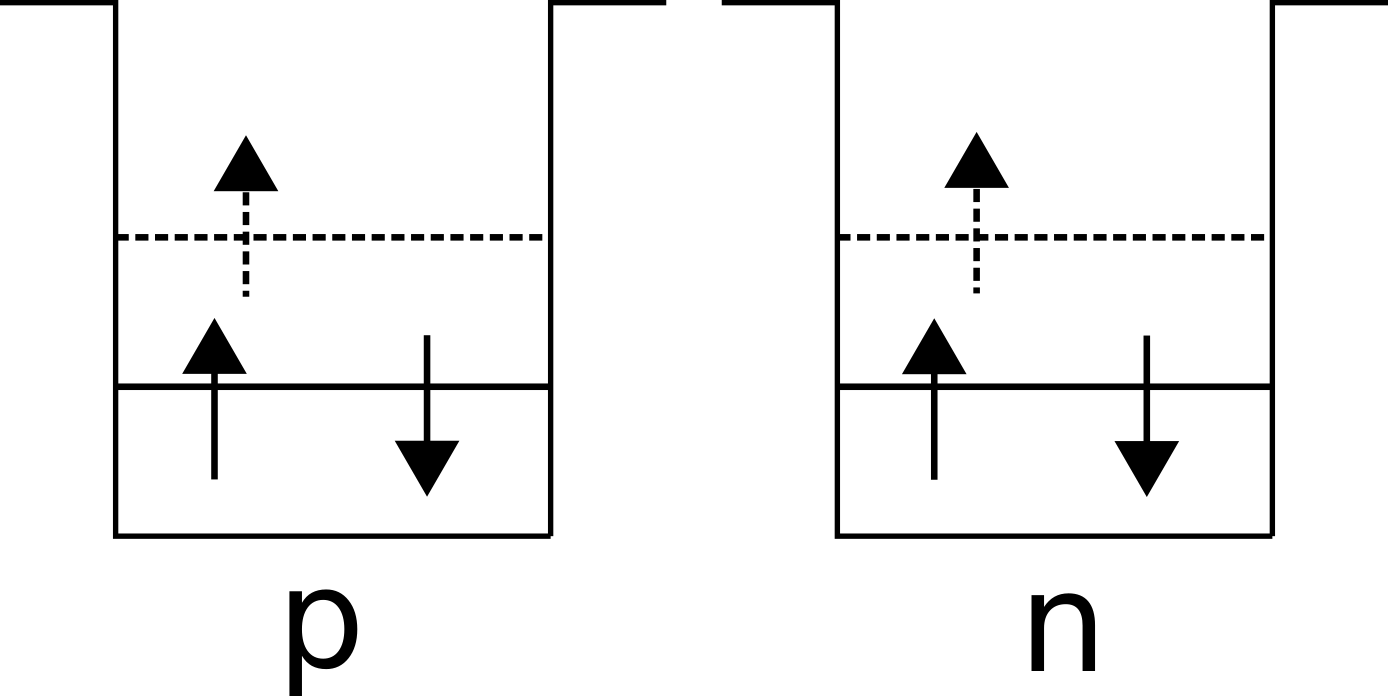
\includegraphics[width=150pt]{fig5_08}
\end{figure}

Quello che la natura ci mostra è però che non esistono nuclei stabili con numero di massa pari ad $A=5$.
Vuol dire che semplicemente la nucleosintesi degli elementi si è fermata all'elio, se fosse esistito un terzo elemento l'evoluzione dell'universo sarebbe stata molto diversa.

\item Un altro effetto spiegabile è il decadimento$\beta$, in particolare il motivo per cui il protone risulta stabile fuori dal nucleo ma può decadere nel caso sia all'interno del nucleo.
Ricordiamo ancora i decadimenti $\beta$
\begin{equation}
\begin{split}
\beta^-:\hspace{0.2cm}n\longrightarrow p+e^-+\bar{\nu_e}\\
\beta^+:\hspace{0.2cm}p\longrightarrow n+e^++\nu_e
\end{split}
\end{equation}
Questo vuol dire semplicemente continuando a mettere protoni oltre il numero di neutroni otterrò nel livello dei neutroni un livello libero e questo causa il decadimento.
\begin{figure}[h]
\centering
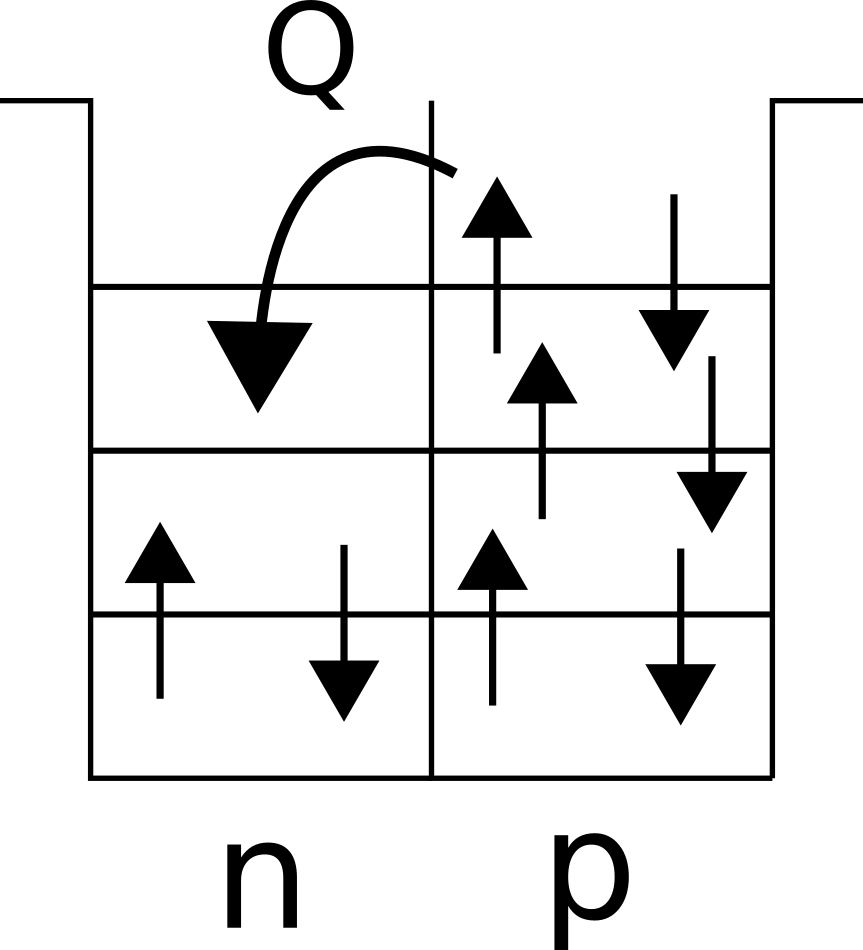
\includegraphics[width=120pt]{fig5_09}
\caption{Decadimento del protone nel nucleo}
\end{figure}

Al di fuori del nucleo non può avvenire in quanto il $Q=M_i-M_f$ della reazione non è favorevole (è negativo), ovvero l'energia di massa del protone fuori dal nucleo è minore dei prodotti della reazione mentre all'interno del nucleo la questione è opposta.
\begin{equation}
\beta^+\hspace{0.2cm}Q=m_p-m_n-m_{e^+}-m_\nu
\end{equation}
Riportiamo quindi le masse del decadimento 
\begin{equation}
\begin{split}
&m_p=938,2\frac{MeV}{c^2}\\
&m_n=939,5\frac{MeV}{c^2}\\
&m_e=0,511\frac{MeV}{c^2}
\end{split}
\end{equation}
Il $Q$ della reazione risulta quindi essere in questo caso
\begin{equation}
Q^{\beta^+}=-1,8MeV
\end{equation}
Questa è una reazione endotermica e quindi non avviene spontaneamente.
Il $Q$ del decadimento del neutrone fuori dal nucleo è invece
\begin{equation}
Q^{\beta^-}=m_n-m_p-m_{e^-}=0,8MeV
\end{equation}
Il neutrone è stabile all'interno del nucleo per il principio di esclusione di Pauli che ne impedisce il decadimento, si ha però, come per il protone, che un eccesso di neutroni porta comunque al decadimento.

\item Nel modello a goccia abbiamo calcolato il libero cammino medio del nucleone nel nucleo corrispondente a $l=0,21fm$.
Nel modello di Fermi invece abbiamo considerato i nucleoni come un gas di particelle libere nel nucleo cioè prive di interazioni.

Queste due visioni apparentemente contrastanti si conciliano in quanto se non ci sono stati liberi le particelle non collidono tra loro (una collisione comporta uno scambio di energia che nella stabilità non vi può essere), quindi non è propriamente vero che il libero cammino medio è una frazione di Fermi poiché  con tutti gli stati occupati le particelle devono considerarsi libere.
\end{itemize}

%nuova sezione--------------------------------------------------
\subsection{Modello a shell}
L'evidenza sperimentale che portò alla costruzione di questo modello si basa sull'analogia con il modello a shell elettroniche dell'atomo. 
Facendo un grafico dell'energia di estrazione di un nucleone in funzione del numero atomico, si vide che aveva lo stesso andamento del grafico del lavoro di estrazione degli elettroni.
Sorge spontaneamente il dubbio che quindi possa avere una struttura a shell pure il nucleo.
\begin{figure}[h]
\centering
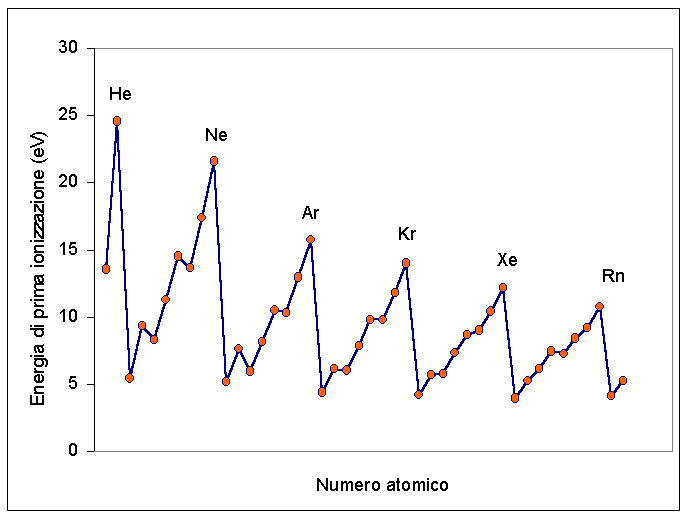
\includegraphics[width=150pt]{fig5_10}
\caption{Lavoro di estrazione elettronico in funzione del materiale}
\end{figure}

Ci sono un paio di differenze tra il modello elettronico e nucleare
\begin{itemize}
\item La prima consiste nell'ordine di grandezza, infatti, mentre per gli elettroni si parla di $eV$ nel caso dei nuclei di $MeV$, consistentemente con quanto già visto.

\item Il secondo è la posizione dei picchi.
Nel caso degli elettroni i picchi corrispondo ai gas nobili, nel caso dei nuclei i picchi corrispondono a 2, 8, 20, 28, 50, 82, 126 (si fa riferimento sia al numero di neutroni che di protoni).
Per esempio con il 20 si può avere il Calcio 40 $^{40}_{20}Ca$.
\end{itemize}

Ciò che non fu subito chiaro è come mai si hanno questi valori di massimo, infatti la struttura dell'atomo rende abbastanza evidente il motivo (regola dell'otteto e livelli energetici delle shell), mentre nel nucleo non c'è un potenziale ben definito che vada a creare dei livelli energetici così chiari in quanto ogni nucleone interagisce con gli altri (e come visto dal modello a goccia con un numero di legami differente).

Per risolvere questo problema bisogna considerare un nucleone e approssimare le interazioni con un potenziale medio.
\begin{figure}[h]
\centering
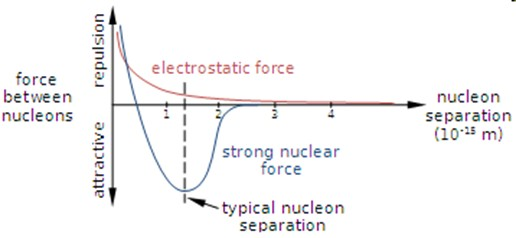
\includegraphics[width=150pt]{fig5_11}
\caption{Potenziale nucleare in funzione del raggio}
\end{figure}

Come si può vedere dal grafico il potenziale nucleare dovrà avere una forma in cui a valori molto bassi di raggio non implode su se stesso, e quindi valore positivo (potenziale repulsivo) ma che poi scende per creare una buca di potenziale negativa che arriva ad azzerarsi quando il raggio è pari al raggio nucleare, il tutto restando sempre in opposizione al potenziale elettrostatico.
Per approssimare questa forma si usa il potenziale di Saxon-Woods dove la forza repulsiva iniziale viene ignorata e la forma è a metà tra la curva e una buca di potenziale rettangolare.
\begin{figure}
\centering
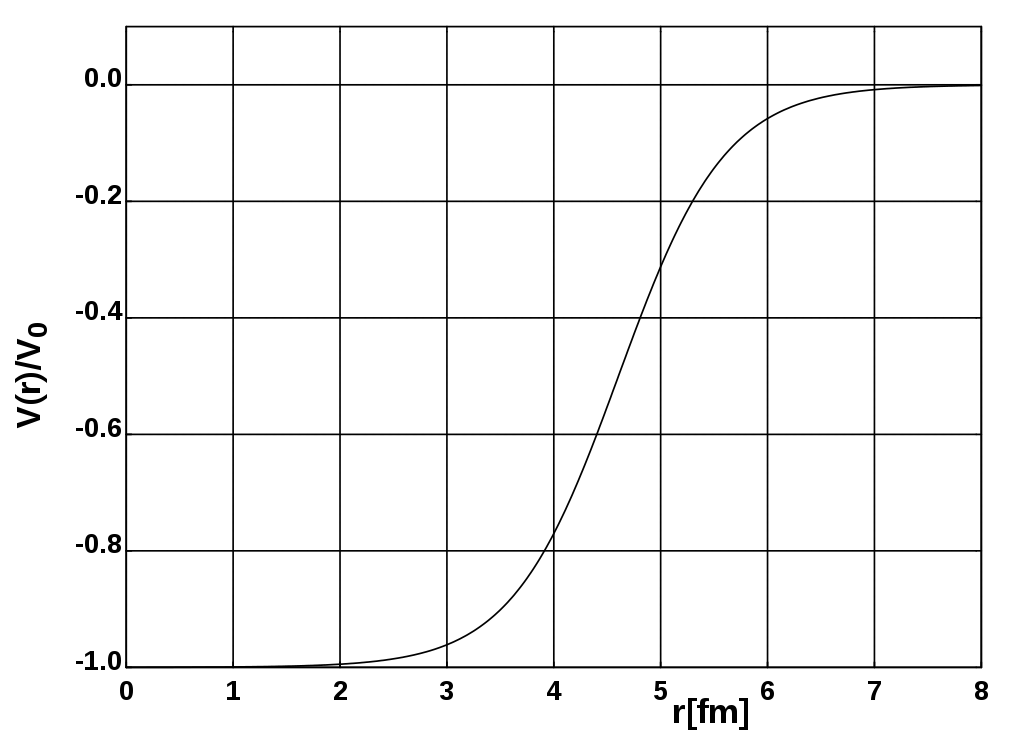
\includegraphics[width=150pt]{fig5_12}
\caption{Potenziale di Saxon-Woods}
\end{figure}

Il potenziale di Saxon-Woods ha formula
\begin{equation}
V=-\frac{V_0}{1+\frac{\exp(r-R)}{a}}
\end{equation}
Dove $V_0=50MeV$, $R=R_0A^{1/3}$ e $a=0,56fm$.

In particolare questo potenziale si differenzia dalla buca di potenziale classica nella regione tra i $3fm$ e i $7fm$ ed è proprio questa regione che determina le caratteristiche dei livelli energetici del nucleo.
\paragraph{Livelli atomici}
I livelli atomici sono caratterizzati da 4 numeri quantici: n, L, m, s.
\begin{equation}
\begin{split}
&\forall n\\
&l=0\to n-1\\
&m\hspace{0.5cm}-l<m<l\\
&s=\pm 1/2
\end{split}
\end{equation}
Le shell atomiche si formano quindi come
\begin{equation}
\begin{split}
n=1\hspace{0.5cm}&l=0\hspace{0.2cm}m_s=0\hspace{0.2cm}s=\pm 1/2\\
n=2\hspace{0.5cm}&l=0\hspace{0.2cm}m_s=0\hspace{0.2cm}s=\pm 1/2\\
&l=1\hspace{0.2cm}m=-1,0,+1\hspace{0.2cm}s=\pm1/2
\end{split}
\end{equation}
Si ha quindi che nel livello corrispondente a $n=1$ si possono avere solo 2 elettroni, mentre nel caso di $n=2$ posso avere 2 elettroni nel livello $l=0$ ma anche 6 nel livello $L=1$ il che mi porta ad avere 8 elettroni totali nel livello $n=2$.
Continuando intuitivamente si vede che per esempio il livello $n=3$ ospiterà 18 elettroni.
Questo restituisce esattamente le configurazioni dei primi 3 gas nobili corrispondenti a $Z=2,10,28$ ovvero i primi tre livelli completi.

Nei nuclei abbiamo visto che questi valori non coincidono con i livelli elettronici infatti i valori sono $Z=2, 8, 20, 28, 50, 82, 126$.
Questo è dovuto al fatto che nei nuclei $l$ non è limitato a $n-1$ e inoltre i nuclei hanno la tendenza ad accoppiare lo spin e il momento angolare introducendo un momento 
\[
j=L+s
\]
che può assumere i valori 
\[
j=1/2, 3/2, 5/2, 7/2, \dots
\]
Si ottiene così che il numero di nucleoni in funzione di $j$ sarà
\begin{equation}
\begin{split}
&j\hspace{0.5cm}n\\
&\frac{1}{2}\hspace{0.5cm}2\\
&\frac{3}{2}\hspace{0.5cm}4\\
&\frac{5}{2}\hspace{0.5cm}6\\
&\frac{7}{2}\hspace{0.5cm}8
\end{split}
\end{equation}
La regola generale è quindi
\begin{equation}
j=\frac{X}{2}\longrightarrow n=X+1
\end{equation}
La nomenclatura è la stessa della fisica atomica.
$l=0, 1, 2, 3, 4$ corrispondono rispettivamente a $s, p, d, f, g$.
Per esempio uno stato quantico potrà essere
\begin{equation}
1p^{3/2}
\end{equation}
dove $1$ è il numero quantico principale, $p$ corrisponde a $l=1$ e $3/2$ indica che in questo stato potrò avere 4 particelle.
Dalle evidenze sperimentali è stato possibile quindi trovare la configurazione di shell del nucleo.
\begin{figure}
\centering
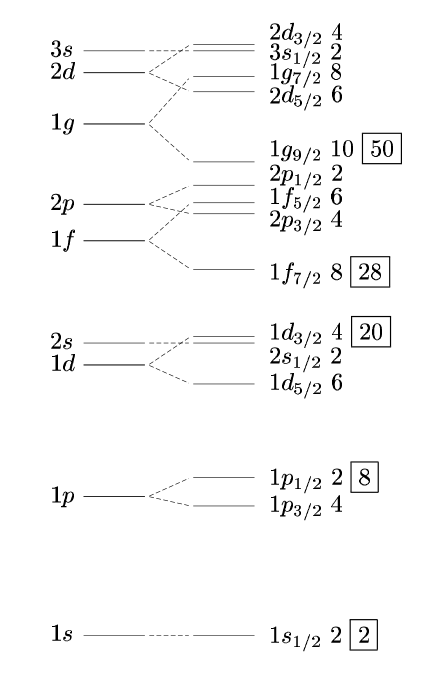
\includegraphics[width=120pt]{fig5_13}
\caption{Struttura delle shell nucleoniche con evidenza sui livelli stabili}
\end{figure}

Quella rappresentata in figura è la schematizzazione dei livelli energetici del nucleo, e si può notare che quindi i nucleoni all'interno del nucleo:
\begin{itemize}
\item non sono posizionati casualmente;
\item hanno momenti angolari;
\item soddisfano la statistica di Fermi e di conseguenza anche al principio di esclusione di Pauli.
\end{itemize}




\section{Applicazioni}
\subsection{Risonanza Magnetica Nucleare}
La risonanza magnetica è una tecnica di imaging medico non invasiva.
Si basa sul fatto che ad ogni protone è associato un piccolo campo magnetico associato al dipolo. 
Ponendo questi dipoli sotto l'azione di un campo magnetico forte, si avrà l'allineamento con il campo, sia nella stessa direzione che i direzione opposta.
\begin{equation}
E=-\bar \mu\cdot \bar B
\end{equation}
Ciò che si otterrà è che l'energia sarà minore se il campo e il dipolo sono solidali ($\mu\uparrow\  B\uparrow$), mentre sarà maggiore nel caso contrario ($\mu\uparrow\  B\downarrow$).
\begin{figure}

\end{figure}
La differenza di energia è pari a $\Delta E=\mu B$.
La risonanza in campo magnetico sfrutta esclusivamente nucleoni ma in altri ambiti possono essere usati anche gli elettroni e dalla formula sopra si può vedere come sia diversa nei due casi.

I valori del magnetone di Bohr e del magnetone nucleare sono 
\begin{equation}
\begin{split}
\mu_B=\frac{e\hbar}{2m_e}=9,3\times10^{-24}\frac{j}{T}=5,8\times10^{-5}\frac{eV}{T}\\
\mu_N=\frac{e\hbar}{2m_p}=5,0\times10^{-27}\frac{j}{T}=3,8\times10^{-8}\frac{eV}{T}
\end{split}
\end{equation}

La risonanza magnetica funziona che una volta applicato un campo magnetico i livelli energetici con spin up e down si dividono e fornendo una radiofrequenza con energia pari alla differenza di energia generata il mio campione assorbirà energia, e io sono sensibile all'energia assorbita. 

Dato un elettrone se applico un campo B=0,335T, ottengo che la differenza di energia sarà pari a $\Delta E=6,22\times 10^{-24}j$.
In questo caso la frequenza coinvolta (assorbita dall'elettrone) è pari a $\nu =9,4GHz$, ovvero nel campo delle microonde.

Nel caso del protone, ovvero quello usato in campo medico, c'è la necessità di applicare un campo magnetico molto più alto per portare ad una separazione sufficientemente visibile. 
Applicando un campo $B=2T$ ottengo $\Delta E=5,64\times10^{-26}j$, vi è quindi la necessità di una radiofrequenza dell'ordine di $\nu =\frac{\Delta E}{h}=85MHz$.

Quello che succede è che pongo il paziente in questi campi magnetici e faccio passare una radiofrequenza. 
L'assorbimento di questa radiofrequenza avviene in funzione della densità del materiale biologico.
Una cosa di cui devo tener conto è l'agitazione termica dei protoni, posso immaginare che maggiore è l'agitazione termica minore sarà il contrasto dell'immagine, una soluzione sarebbe abbassare la temperatura ma non potendo congelare il paziente non resta che sfruttare campi magnetici molto forti($\Delta E/KT$).
Il segnale che io rivelo è proporzionale alla densità di protoni, le zone più chiare sono quelle a più elevata densità di protoni.
Per avere una risoluzione spaziale, ovvero una tridimensionalità, applico un gradiente di campo magnetico minimo che produrrà una risonanza diversa a diverse frequenze di radiofrequenza generando una variazione ulteriore che mi permette di ampliare l'imaging.
Per andare ad aumentare il contrasto andrò a vedere la risposta temporale del campione.
Quando irradio il tessuto i protoni assorbendo energia passeranno da uno stato all'altro (spin-flip), se poi io fermo la radiazione e lascio il tessuto tornare allo stato fondamentale potrò poi misurare il tempo impiegato per la diseccitazione e avrò quindi informazioni addizionali sul tessuto che circonda il materiale in analisi.



%%
%% Author: dariochinelli
%% 2021-04-21
%%

\section{Potenziale nucleare}
Studiamo il potenziale nucleare considerando il nucleo del \emph{deuterio}, chiamato \emph{deutone}, composto da un protone ed un neutrone.

\paragraph{La Cromodinamica Quantistica (QCD)} è una teoria quantistica di campo e relativistica, è una teoria fondamentale che spiega l'interazione tra particelle elementari.
I nucleoni, i componenti del nucleo, protone e neutrone, sono a loro volta composti da \emph{quark}, i quali sono particelle elementari prive di dimensione e con carica frazionaria
\begin{itemize}
\item quark up $u$ ha carica $+\frac{2}{3}$
\item quark down $d$ ha carica $-\frac{1}{3}$
\end{itemize}
i nucleoni sono composti da 3 quark ciascuno e seguono la regola per cui
\begin{itemize}
\item il \textbf{protone} è composto da due quark \emph{up} ed un quark \emph{down}, ha quindi carica totale unitaria:
$$u+u+d = +\frac{2}{3} +\frac{2}{3} -\frac{1}{3} = 1$$
\item il \textbf{neutrone} è composto da due quark \emph{down} ed un quark \emph{up}, ha quindi carica totale nulla:
$$d+d+u = -\frac{1}{3} -\frac{1}{3} +\frac{2}{3} = 0$$
\end{itemize}
\begin{figure}[h]
\centering
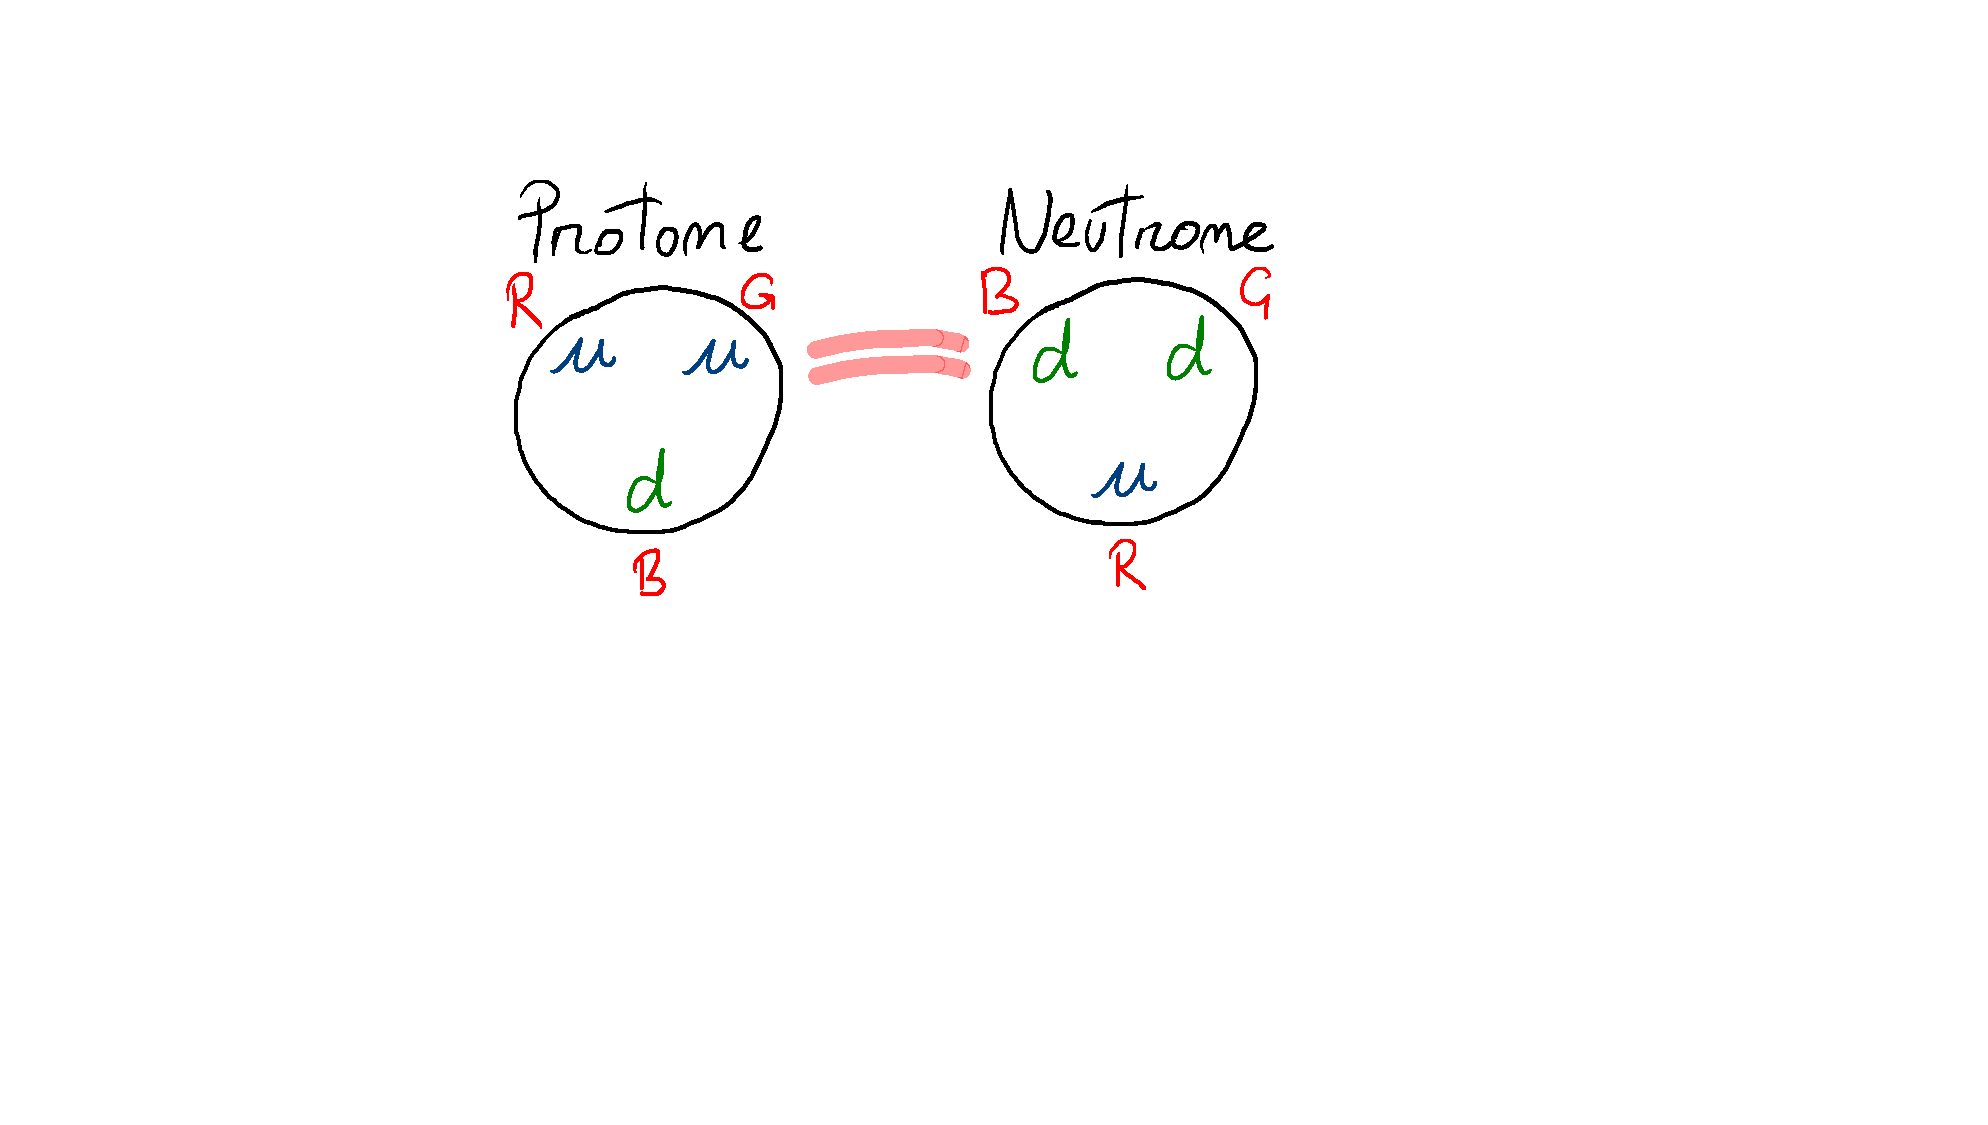
\includegraphics[scale=0.5]{/protone_neutrone_quark}
\caption{CAPTION}
\end{figure}

\paragraph{Carica di colore} I quark hanno anche un secondo tipo di carica: la \emph{carica di colore} che regola l'\emph{interazione forte} tra i quark.
La carica di colore può essere di tre tipi: Red (R), Green (G), Blue (B).
La somma delle tre cariche di colore dei rispettivi quark di un nucleone è nulla
\begin{equation}
R + G + B = 0
\end{equation}
un quark rosso (R) attira un quark verde (G) che attira un quark blu (B), mentre i quark dello stesso colore si respingono.
La teoria fondamentale della QCD esprime come l'interazione nucleare si possa interpretare come la carica di colore residua.

\paragraph{Il potenziale tra nucleoni} è un potenziale di interazione del tipo
\begin{figure}[h]
\centering
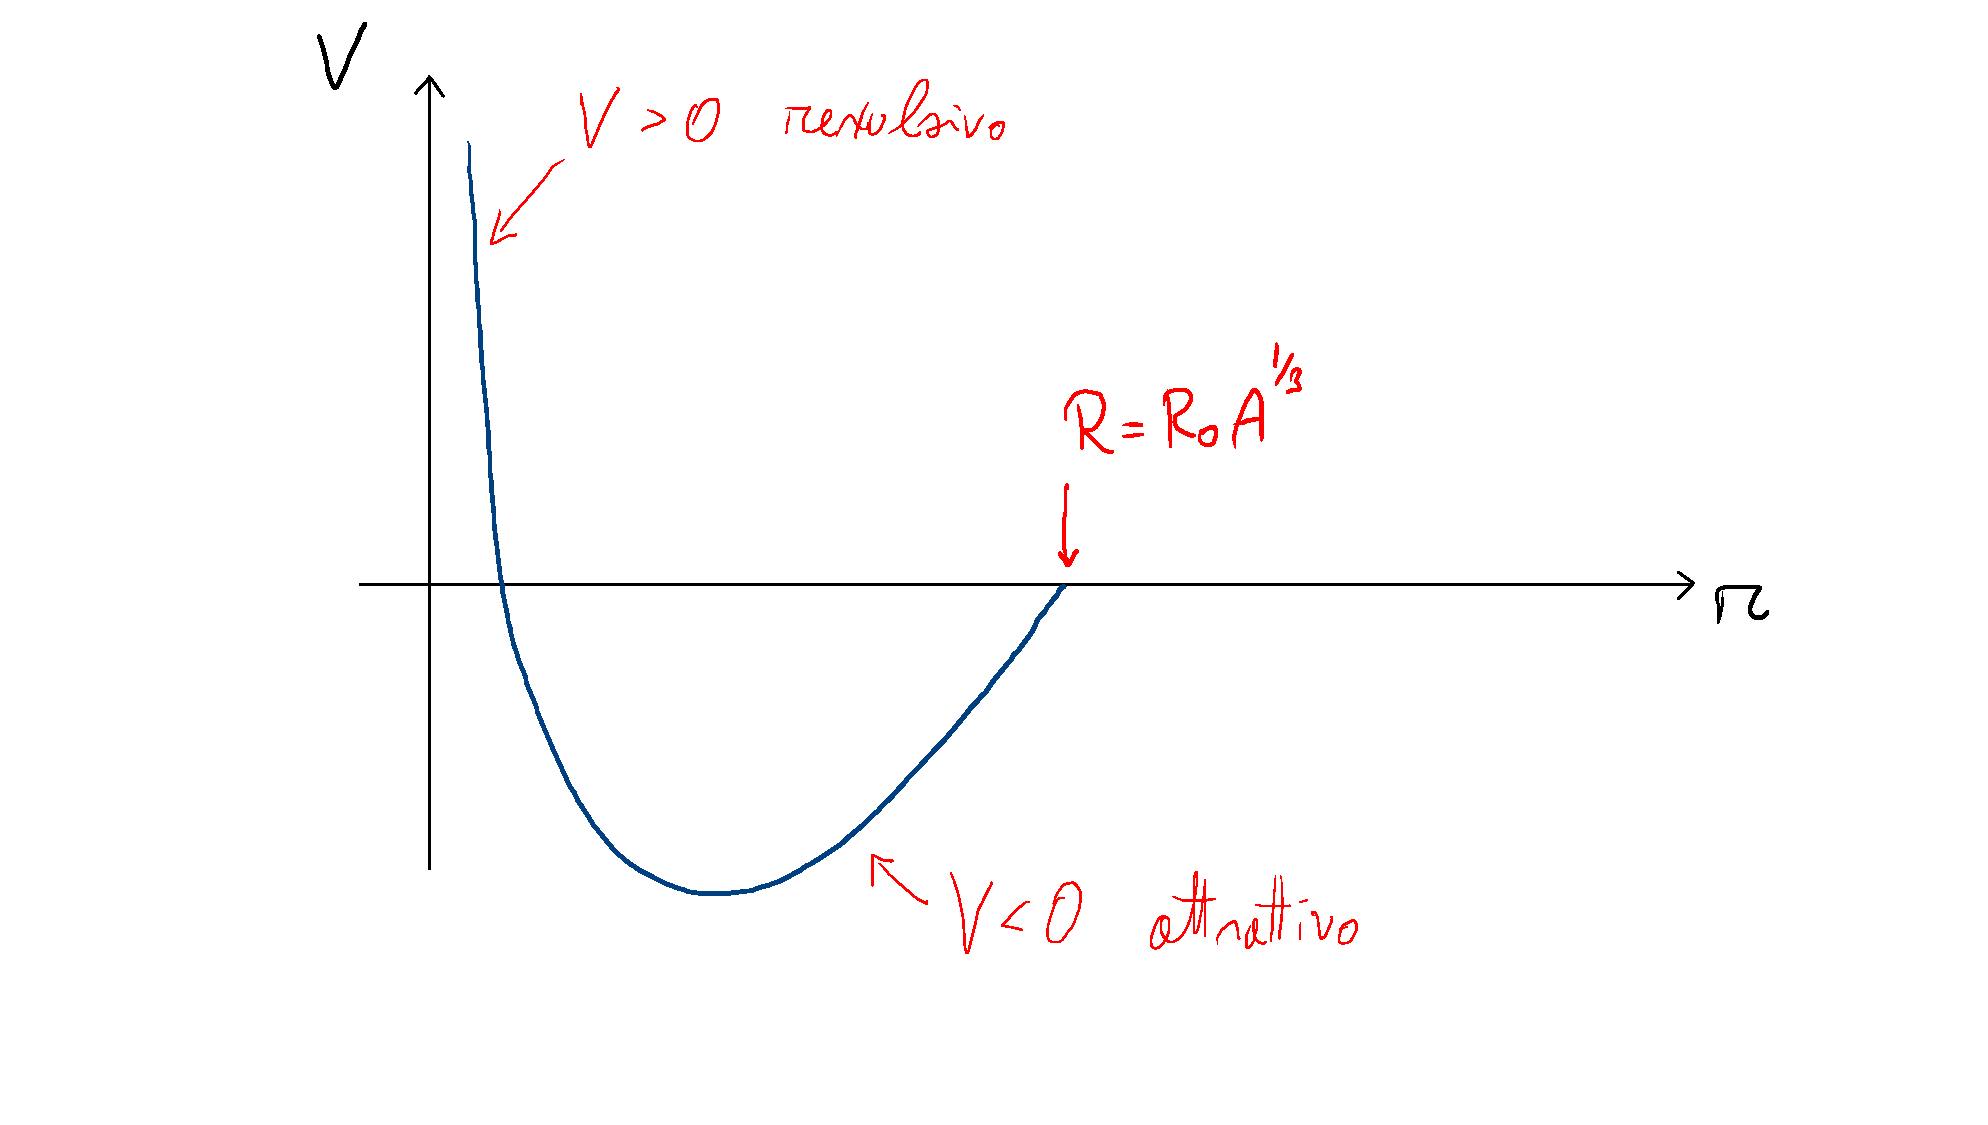
\includegraphics[scale=0.4]{/potenziale_nucleare_1}
\caption{CAPTION}
\end{figure}
Nella prima parte del potenziale si ha che per piccole distanze è \emph{positivo}, ovvero repulsivo, poiché altrimenti i nuclei \underline{privi di dimensione (?)} collasserebbero, ciò è legato al Principio di Esclusione di Pauli, nella seconda parte il potenziale è \emph{attrattivo} ed è ciò che "intrappola" i nucleoni all'interno del nucleo, inoltre oltre alla distanza data da $R = R_0 A^{\frac{1}{3}}$ la forza nucleare è nulla.

\paragraph{Il Deutone} è il nucleo del deuterio, è composto da un protone e un neutrone ed è il più semplice nucleo su cui studiare la forza nucleare.
Del deutone conosciamo l'energia di legame $E_B = \SI{-2.225}{MeV}$ e la distanza tra i nucleoni $R = \SI{2.1}{fm}$ ottenuti sperimentalmente.
Conosciamo inoltre che lo stato legato del deuterio è quello in cui gli spin sono paralleli, dato ottenuto dalla misurazione del momento magnetico, per cui lo spin del deutone è $S = 1$.
\begin{figure}[h]
\centering
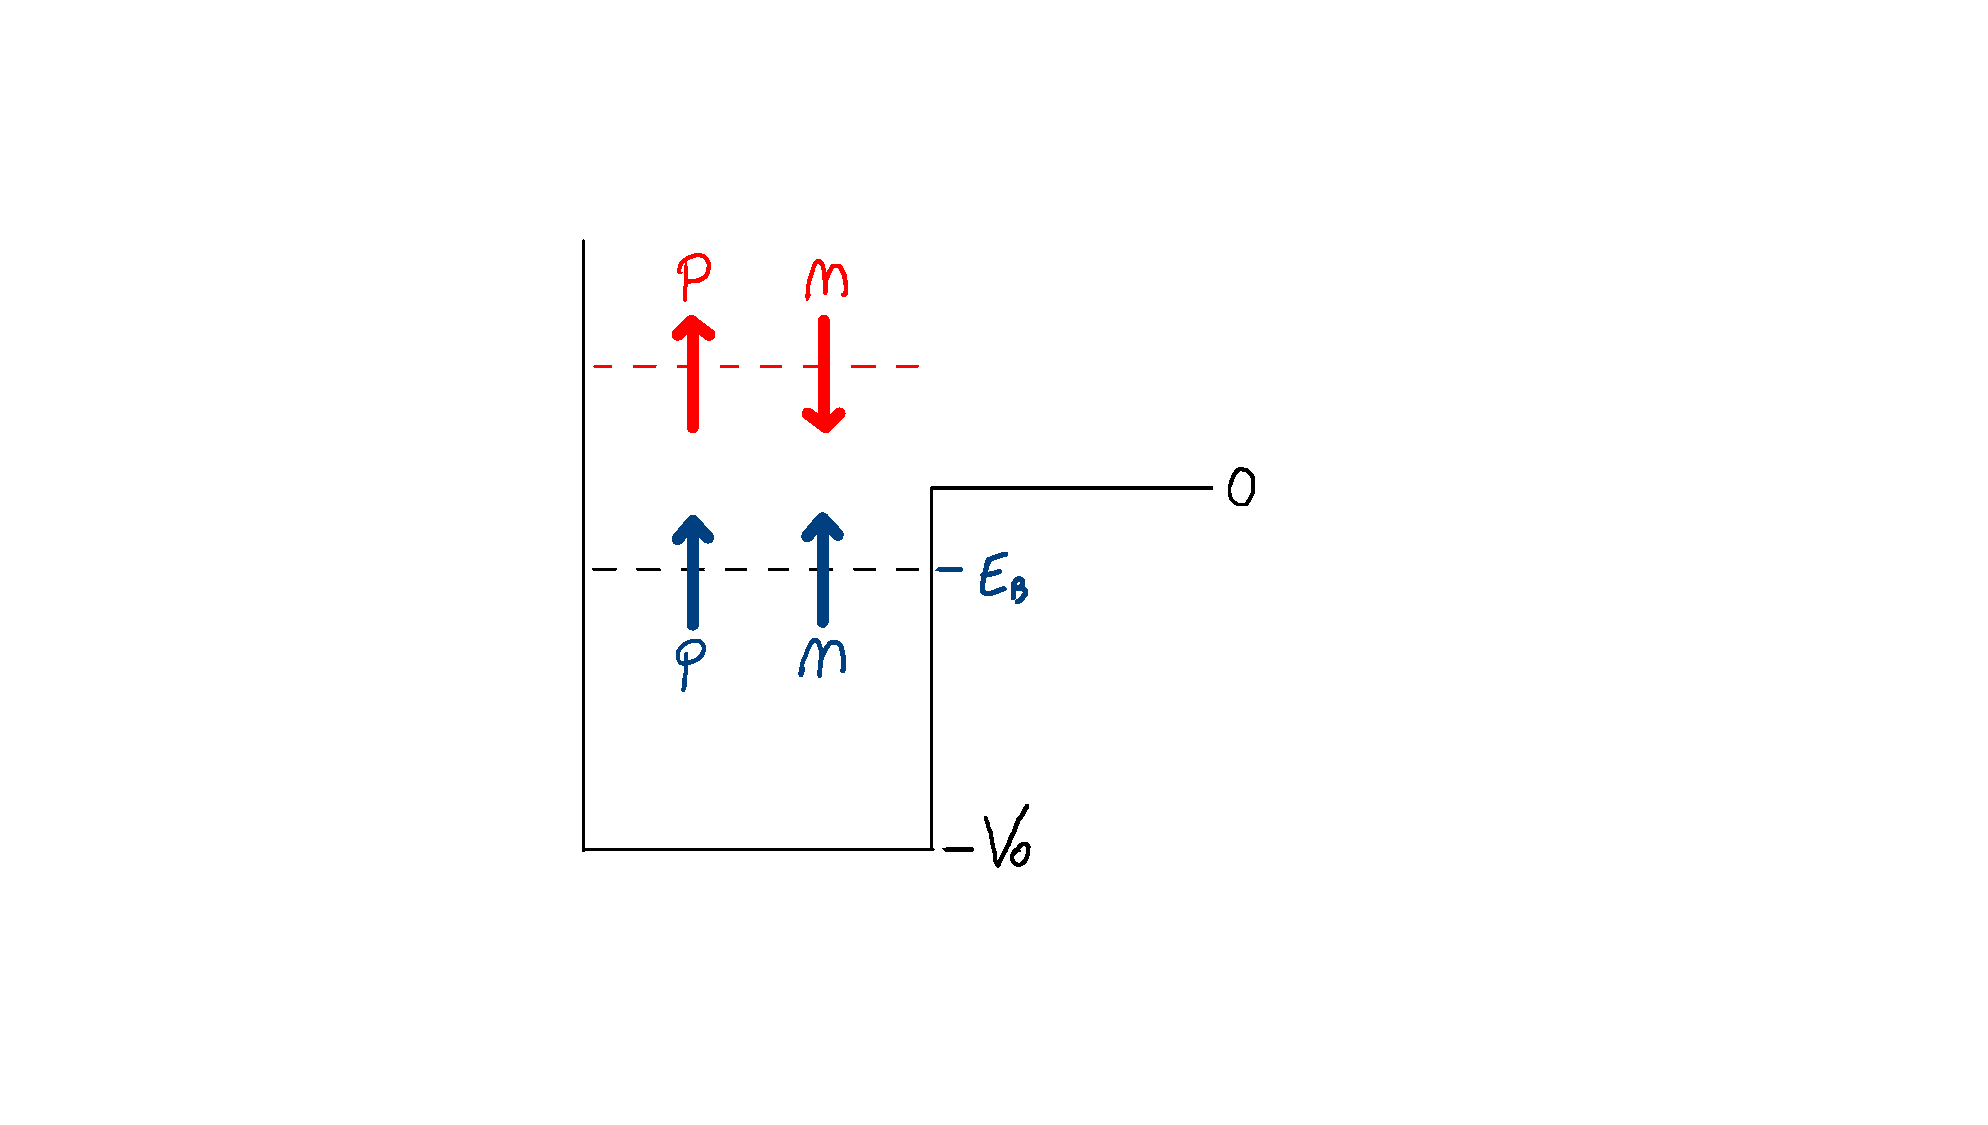
\includegraphics[scale=0.5]{/spin_deutone}
\caption{CAPTION}
\end{figure}
Uno stato con spin anti-parallelo corrisponde ad uno stato non legato, quindi fuori dalla buca di potenziale.
L'interazione nucleare dipende fortemente dallo spin.

Cerco ora il valore della buca di potenziale $V_0$, sommo l'energia cinetica $KE$ con l'energia potenziale $PE$
\begin{equation}
\begin{split}
E & = KE + PE \\
E_B & = KE + V_0
\end{split}
\end{equation}
scrivendo la funzione d'onda trovo il legame con il potenziale $V$
\begin{equation}
\begin{split}
H \psi & = E \psi \\
- \frac{\hbar^2}{2m} \frac{d^2}{dr^2} \psi + V \psi & = E \psi
\end{split}
\end{equation}
Il potenziale di questa buca è
\begin{equation}
V = 
\Bigg\{\begin{array}{l}
V_0 \quad\mbox{zona \Romannum{1}: dentro la buca} \\
0 \quad\mbox{ zona \Romannum{2}: altrove}
\end{array}
\end{equation}
Scrivo l'equazione di Schrodinger nella zona \Romannum{1}, in cui ho $V = V_0$
\begin{equation}
\begin{split}
- \frac{\hbar^2}{2m} \frac{d^2 \psi}{d r^2} + V_0 \psi & = E \psi \\
\frac{d^2 \psi}{d r^2} & = -\frac{2m}{\hbar^2} (E - V_0) \psi \\
\frac{d^2 \psi}{d r^2} & = - K^2 \psi \quad\quad \mbox{con } K^2 = \frac{2m}{\hbar^2} (E - V_0)
\end{split}
\end{equation}
la soluzione ha un andamento oscillatorio ed in generale è
\begin{equation}
\psi(r) = A \sin Kr + B \cos Kr
\end{equation}
calcolo $A$ e $B$ imponendo le condizioni al contorno:
\begin{equation}
\psi (0) = 0 \quad\Rightarrow\quad \psi(0) = A \sin 0 + B \cos 0 = 0 \quad\Rightarrow\quad B=0
\end{equation}
per cui diventa
\begin{equation}
\psi = A \sin K r
\label{psi_1}
\end{equation}
Scrivo l'equazione di Schrodinger nella zona \Romannum{2}, in cui ho $V =0$
\begin{equation}
\begin{split}
\frac{d^2 \psi}{d r^2} & = -\frac{2m}{\hbar^2} E \psi \\
\frac{d^2 \psi}{d r^2} & = L^2 \psi \quad\quad \mbox{con } L^2 = - \frac{2m}{\hbar^2} E
\end{split}
\end{equation}
la soluzione ha un andamento esponenziale ed in generale è
\begin{equation}
\psi(r) = C e^{L r} + D e^{- L r}
\end{equation}
di cui so che deve appartenere allo spazio di Hilbert, per cui la parte $e^{L r}$ non è soluzione in quanto non verifica la condizione $|\psi|^2 < \infty$, per cui diventa
\begin{equation}
\psi(r) = D e^{- L r} 
\label{psi_2}
\end{equation}
Eguagliando le funzioni d'onda \ref{psi_1} e \ref{psi_2} e le loro derivate in corrispondenza della frontiera $r = R$ trovo
\begin{equation}
\Bigg\{\begin{array}{l}
\psi_{\Romannum{1}}(R) = \psi_{\Romannum{2}}(R)\\
\psi_{\Romannum{1}}'(R) = \psi_{\Romannum{2}}'(R)
\end{array}
\quad\Rightarrow\quad 
\Bigg\{\begin{array}{l}
A \sin K R = D e^{ - L R }\\
K A \sin K R = -L D e^{ - L R }
\end{array}
\end{equation}
dividendo una con l'altra le equazioni del sistema trovo la relazione seguente in funzione dei parametri $K$ ed $L$
\begin{equation}
\begin{split}
K & = \sqrt{\frac{2m}{\hbar^2} (E - V_0)} \in \mathbb{R} \\
L & = \sqrt{- \frac{2m}{\hbar^2} E} \in \mathbb{R}
\end{split}
\end{equation}
che quindi diventa
\begin{equation}
\begin{split}
& K \cot K R = - L \\
& \sqrt{\frac{2m}{\hbar^2} (E - V_0)} \cot \Bigl[ R \sqrt{\frac{2m}{\hbar^2} (E - V_0)} \Bigr] = - \sqrt{- \frac{2m}{\hbar^2} E}
\end{split}
\end{equation}
da cui, inserendo i dati sperimentali, 
\begin{equation}
\begin{split}
E & = \SI{-2.225}{MeV} \\
R & = \SI{2.1}{fm}
\end{split}
\end{equation}
e la massa corrisponde alla massa ridotta tra il protone ed il neutrone
\begin{equation}
m = \frac{m_n m_p}{m_n + m_p} \simeq \frac{m_p^2}{2 m_p} = \frac{m_p}{2}
\end{equation}
trovo il valore della buca di potenziale
\begin{equation}
V_0 = \SI{-36}{MeV}
\end{equation}
(non è ben noto come sia davvero possibile risolvere l'equazione del tipo $x \cot a x = b$ ma ok, prendiamo atto del risultato precedente e andiamo avanti).

Risulta quindi che la buca di potenziale del Deutone è profonda $\SI{-36}{MeV}$ di cui solo $\SI{-2.225}{MeV}$ sono di energia potenziale, \emph{di legame}, mentre circa $\SI{-34}{MeV}$ sono di energia cinetica.

Per il ferro $^{56}_{26}Fe$ ad esempio si ha un'energia di legame media di circa $\SI{8}{MeV / nucleone}$, mentre
per il deutone $^{2}_{1}He$ si ha circa $\SI{1.1}{MeV / nucleone}$.

Troviamo tre punti notevoli della funzione d'onda:

\begin{itemize}
\item Quanto vale la funzione d'onda nel punto $r=R$?
In tale punto la funzione vale $\sin K R$ per cui conoscendo i dati trovo
\begin{equation}
\begin{split}
& R = \SI{2.1}{fm} \\
& K = \sqrt{ \frac{2m}{\hbar^2} (E - V_0) } \simeq \SI{0.9}{fm^{-1}} \\
& \sin K R = \sin (0.9 \cdot 2.1) = 0.95
\end{split}
\end{equation}

\item In che punto si ha il valore massimo della funzione d'onda?
\begin{equation}
\begin{split}
& \sin K r = 1 \\
& K r = \frac{\pi}{2} \\
& r = \frac{\pi}{2} \frac{1}{K} \simeq \SI{1.74}{fm}
\end{split}
\end{equation}

\item In che punto la funzione d'onda vale circa $\frac{1}{3}$?
\begin{equation}
\begin{split}
e^{ - L r } & \quad L = \sqrt{\frac{2mE}{\hbar^2}} \to \frac{1}{L} = \SI{4.4}{fm} \\
e^{ - L r } & \rightarrow e^{ \frac{-L}{L}} = e^{ -1 } = 0.37
\end{split}
\end{equation}
\end{itemize}
La funzione d'onda ottenuta evidenzia come sia possible trovare la particella al di fuori della buca di potenziale, a distanze oltre i $\SI{5}{fm}$.











%%% Dario Chinelli 24/05/21

\section{Decadimenti nucleari}
La formula semi-emipirica di massa, equazione \ref{formula_semiempirica_massa} nei capitoli precedenti, esprime la stabilità o instabilità dei nuclei nel caso in cui ci sia un'abbondanza di neutroni o di protoni.
Per basi numeri atomici il numero di protoni e di neutroni si equivale, aumentando il numero di massa i nuclei tendono ad avere più neutroni che protoni ed in particolare i nuclei stabili e arrivano ad un numero atomico di circa 80 ed un numero di neutroni di circa 110.
Tutti gli atomi con elevato numero atomico e di massa sono instabili, come ad esempio l'uranio che ha numero atomico 92 ed è un elemento instabile che si trova in natura.
\begin{figure}[h]
\centering
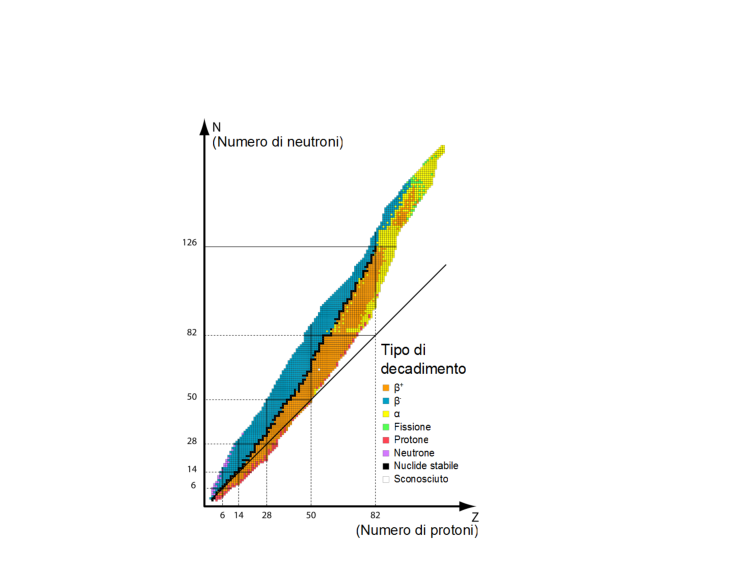
\includegraphics[scale=1]{/nuclei_stabili}
\caption{Il grafico rappresenta per quali combinazioni di neutroni e protoni si hanno atomi stabili.}
\end{figure}
Il decadimento dei nuclei avviene spontaneamente in alcune circostanze

\begin{enumerate}
\item  il nucleo ha troppi neutroni, allora si ha un processo di decadimento beta $\beta^-$
\begin{equation}
^{A}_{Z}X \quad\longrightarrow\quad  ^{A}_{Z+1}X + e^- + \bar\nu_e
\end{equation}
dopo il decadimento si ha un atomo della stessa specie X.
Questo processo è descritto in dettaglio da un decadimento di un neutrone
\begin{equation}
n \quad\longrightarrow\quad p + e^- + \bar\nu_e
\end{equation}
a livello di quark tale processo consiste nella conversione di un quark down in un quark up
\begin{equation}
d \quad\longrightarrow\quad u + e^- + \bar\nu_e
\end{equation}
mediato dal bosone $W$, mediatore della forza debole.

\item il nucleo può avere troppi protoni, si ha allora un processo di decadimento beta $\beta^+$
\begin{equation}
^{A}_{Z}X \quad\longrightarrow\quad ^{A}_{Z-1}Y + e^+ + \nu_e
\end{equation}
dopo il decadimento si ha un atomo di una diversa specie atomica.
Nel dettaglio vediamo che questo processo è descritto dal decadimento di un protone
\begin{equation}
p \quad\longrightarrow\quad n + e^+ + \nu_e
\end{equation}
e a livello di quark 
\begin{equation}
u \quad\longrightarrow\quad d + e^+ + \nu_e
\end{equation}

\item se ci sono troppi nucleoni, quindi siamo nella parte alta del grafico, i nuclei tendono a subire un processo di decadimento alpha $\alpha$, una particella alpha è un nucleo di Elio
\begin{equation}
^{A}_{Z}X \quad\longrightarrow\quad ^{A-4}_{Z-2}Y + \alpha
\end{equation}

\item il nucleo potrebbe avere anche troppa energia, quindi nel caso di un nucleo eccitato $X^{\ast}$, si ha emissione di radiazione elettromagnetica chiamata \emph{radiazione gamma}
\begin{equation}
^{A}_{Z}X^{\ast} \quad\longrightarrow\quad ^{A}_{Z}X + \gamma
\end{equation}

\item nel caso in cui le energie di eccitazione siano molto elevate si può avere decadimento per \emph{fissione} 
\end{enumerate}

Le leggi che descrivono un decadimento impongono la conservazione di 
\begin{itemize}
\item energia
\item quantità di moto
\item carica elettrica
\item numero di nucleoni
\item numero di leptoni
\end{itemize}
la massa invece non si conserva nei processi di decadimento.

\paragraph{esempio} utilizzando la formula semi-empirica di massa si verifichi se il decadimento $\alpha$ del $^{238}_{92} U$ sia possibile energeticamente.

La massa totale iniziale del sistema deve essere maggiore della massa totale finale, allora il processo è esotermico.
$$ M_i > M_f \quad\Rightarrow\quad esotermico $$
\begin{equation}
^{238}_{92} U \quad\longrightarrow\quad ^{234}_{90}X + ^{4}_{2}He
\end{equation}
(l'elemento figlio di questa reazione è un isotopo del Torio $^{232}_{90}Th$, ma non è importante ai fini della trattazione)
dobbiamo calcolare il $Q$ della reazione e ci chiediamo se è maggiore di zero
\begin{equation}
Q = M(A,Z) - M(A-4,Z-2) - M(^{4}_{2}He^{++}) > 0
\end{equation}
la massa dell'atomo iniziale equivale a
\begin{equation}
M(A,Z) = Z M_H + (A-Z)M_n - B(A,Z)
\end{equation}
dove $B$ rappresenta l'energia di legame
quindi il calore nella reazione è
\begin{equation}
\begin{split}
Q  & = -B(A,Z) + B(A-4,Z-2) + B(^{4}_{2}He^{ ++ }) \\
& = [ -1807.5 + (1784 + 32.85)] MeV = \SI{9.35}{MeV} > 0
\end{split}
\end{equation}
risulta quindi positivo, per cui il decadimento alpha è energeticamente possibile, anzi avviene spontaneamente; questo calcolo non ci dice nulla però sulla probabilità che avvenga.
La natura tende a minimizzare la massa.

Ci si può divertire con un programma in MathLab delle slide calcolando l'energia di legame per tutti i nuclei...
si trova l'andamento del calore Q emesso/assorbito dalla reazione in funzione del numero atomico, vedi figura \ref{calore_vs_numatomico}
\begin{figure}[h]
\centering
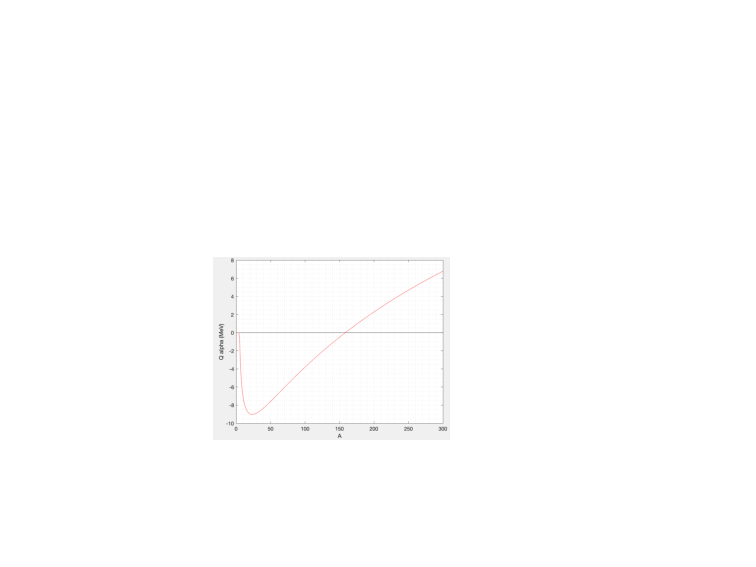
\includegraphics[scale=3]{/calore_vs_numatomico}
\caption{Andamento del calore in funzione del numero atomico}
\label{calore_vs_numatomico}
\end{figure}

\paragraph{esempio} si verifichi se l'Uranio $^{238}_{92}U$ possa decadere $\beta^-$
\begin{equation}
^{238}_{92}U \quad\longrightarrow\quad ^{238}_{92}U + ^{238}_{93}U + e^- + \bar\nu_e
\end{equation}
ovvero ci si chiede se il calore della reazione è maggiore di zero
\begin{equation}
\begin{split}
Q & = M(A,Z) - M(A,Z+1) \quad\quad > 0 \quad ? \\
& = -B(A,Z) + B(A,Z+1) + (M_H - M_n) \\
& = -1807.5 + 1805 + (-0.78) = - \SI{3.28}{MeV} < 0
\end{split}
\end{equation}
l'uranio non decade spontaneamente $\beta^-$.


\subsection{Legge del decadimento radioattivo}
Il numero di decadimenti al secondo è proporzionale al numero di atomi contenuti nel campione.
$$\frac{decad}{s} \propto atom$$
Introduco la \emph{costante di decadimento} $\lambda$, che mi permette di riscrivere la formula precedente come
\begin{equation}
\frac{dN}{dt} = - \lambda N
\end{equation}
questa è un'equazione differenziale risolvibile tramite separazione delle variabili, che descrive la probabilità che un atomo decada nell'unità di tempo
\begin{equation}
\begin{split}
\frac{dN}{N} & = - \lambda dt \\
\ln N & = -\lambda t + C \\
N & = e^{-\lambda t + C} = e^{-\lambda t } e^C 
\end{split}
\end{equation}
trovo la costante di integrazione $C$, imponendo che al tempo $t=0$ il numero totale di atomi sia $N=N_0$,
quindi ottengo $N_0 = 1 e^C$, da cui scriverò
\begin{equation}
N = N_0 e^{-\lambda t} 
\label{eq_decad}
\end{equation}

Il decadimento viene descritto anche da altre quantità, come il \emph{tempo di dimezzamento} $T_{1/2}$: cioè il tempo dopo il quale il numero di neuclidi iniziali si è dimezzato, ovvero $N = N_0 / 2$ e quindi $t= T_{1/2}$
\begin{equation}
\begin{split}
& \frac{N_0}{2} = N_0 e^{-\lambda T_{1/2}} \\
& 2 = e^{ \lambda T_{1/2} } \\
& T_{1/2} = \frac{\ln 2}{\lambda} \simeq \frac{0.693}{\lambda}
\end{split}
\end{equation}
questo tipo di decadimento esponenziale è un processo puramente quantistico, un essere vivente non ha questi problemi... (lol)

Un'altra quantità importante è detta \emph{vita media} $\tau$: 
\begin{equation}
\begin{split}
\tau & = \frac{\int_{N_0}^{0} t dN}{N_0}  = \frac{1}{N_0} \int_0^{\infty} t (-\lambda N_0 e^{ -\lambda t })dt \\
& = - \lambda \Bigl[  \frac{t (-e^{-\lambda t})}{\lambda} - \int \frac{(1) (-e^{ -\lambda t })}{\lambda} \Bigr]_0^{\infty} \\
& = - \lambda \Bigl[  \frac{- t e^{-\lambda t}}{\lambda} - \frac{ e^{ -\lambda t }}{\lambda^2} \Bigr]_0^{\infty} \\
& = \frac{1}{\lambda}
\end{split}
\end{equation}
per cui la vita media corrisponde all'inverso della costante di decadimento e anche a
\begin{equation}
\tau = \frac{1}{\lambda} = \frac{T_{1/2}}{\ln 2} = 1.44 \cdot T_{1/2}
\end{equation}
che corrisponde al momento in cui il numero di neuclidi è sceso al $37\%$ rispetto al valore iniziale.

È da notare che essendo questo un fenomeno quantistico è quindi anche casuale, ciò che sappiamo è che \emph{mediamente} decadono una certa quantità di nuclei ma non sappiamo quali ne quando succederà.
Il tempo di decadimento è indipendente dalla vita del nucleo, per cui esso può decadere immediatamente oppure non decadere mai. 
Ciò differisce nettamente dallo studio di sistemi biologici, che seguono regole più deterministiche.
Seguendo la \ref{eq_decad}, se ci si aspetta $\Delta N $ eventi in un secondo, tale numero di eventi potrà variare, statisticamente rispetto alla media, seguendo la statistica di Poisson in un intervallo dato da
\begin{equation}
\Delta N - \sqrt{\Delta N} < \Delta N < \Delta N + \sqrt{\Delta N}
\end{equation}
nel $67\%$ dei casi il numero di decadimenti sarà compreso in questo intervallo, ma non è una grandezza deterministica.

\paragraph{esempio} supponiamo di avere $10^{12}$ nuclei con una vita media di $\tau = \SI{e10}{s}$, 
quanti decadimenti si hanno in un secondo?
\begin{equation}
\frac{10^{12}}{10^{10}} - \sqrt{\frac{10^{12}}{10^{10}} } < \Delta N < \frac{10^{12}}{10^{10}} + \sqrt{\frac{10^{12}}{10^{10}} } \quad\Rightarrow\quad 90 < \Delta N < 110
\end{equation}
abbiamo in questo caso una precisione del $10\%$.

Nei processi di decadimento molto rari si utilizza la statistica di Poisson.
\paragraph{esempio} se ho $\Delta n$ al secondo che probabilità ho di registrare $K$ eventi? (se $\Delta n$ è piccolo, con bassa costante di decadimento) la probabilità in questo caso è data dalla statistica di Poisson
\begin{equation}
P(\Delta n, K) = \frac{\Delta n^K}{K!} e^{ -\Delta n }
\end{equation}

\subsection{Catene di decadimento}
Normalmente i decadimenti avvengono in cascata e sono dominate da un sistema di equazioni differenziali, tali equazioni sono chiamate \emph{equazioni di Bateman}
\begin{equation}
\begin{split}
& \frac{dN_1}{dt} = - \lambda_1 N_1(t) \\
& \frac{dN_2}{dt} = - \lambda_1 N_1(t) - \lambda_2 N_2(t) \\
& \frac{dN_i}{dt} = - \lambda_{i-1} N_{i-1}(t) - \lambda_i N_i(t) \\
& \frac{dN_k}{dt} = - \lambda_{k-1} N_{k-1}(t)
\end{split}
\label{bateman_equations}
\end{equation}

\paragraph{esempio} Un nucleo di Uranio che fa \emph{fissione} si divide in due nuclei che hanno circa la metà del numero di massa iniziale. I prodotti di fissione sono radioattivi perché il numero di neutroni è maggiore di quello della stabilità in quanto arrivano da un nucleo con un grande numero di massa.

\subsection{Dose di radioattività}
Il numero di decadimenti al secondo viene chiamato \emph{attività di una sorgente} ed è espresso come 
$$ A = \frac{dN}{dt} = \lambda N $$ 
l'unità di misura è il \emph{Becuerel [Bq]} e corrisponde ad un decadimento al secondo
$$ \SI{1}{Bq} = \frac{1 \quad deca}{1 \quad s} $$
un'unità di misura obsoleta ma ancora utilizzata è il \emph{Courie [Cu]}
$$ \SI{1}{Cu} = \SI{3.7e10}{Bq} $$

\paragraph{esempio} Si calcoli l'attività di $\SI{1}{g}$ di Radio $^{226}_{88} Ra_{138}$.
Il Radio decade $\alpha$ con un tempo di dimezzamento di $T_{1/2} = \SI{1.602}{anni}$ e una vita media di $\tau_{Ra} = \SI{7.3e10}{s} \simeq \SI{2400}{anni}$ e la sua attività è data da
\begin{equation}
A = \frac{N_A}{\tau} = \frac{1}{226} \cdot \frac{\SI{6.02e23}{}}{\SI{7.3e10}{s}} = \SI{3.7e10}{s^{-1}}
\end{equation}

\subsubsection{Radioattività naturale}
\paragraph{Corpo umano} Nel corpo umano sono presenti alcuni isotopi radioattivi, tra cui il Potassio [K] ed il Carbonio [C].
L'isotopo radioattivo del Potassio è il $^{40}_{19}K$ ed è il residuo della formazione terrestre, per cui viene detto Potassio primordiale, un altro isotopo presente nel nostro corpo è il Carbonio $^{14}_{6}C$, che non ha origini primordiali ma si forma nell'alta atmosfera "per bombardamento", e decadono entrambi con un decadimento $\beta$.
Il numero di decadimenti medi nel nostro corpo è pari a $\SI{3700}{Bq}$ e derivano dal $^{40}_{19}K$ e dal $^{14}_{6}C$.
\paragraph{Suolo} L'attività del suolo è pari a $\SI{400}{Bq}$, dovuta dagli elementi $^{40}K$, $^{226}Ra$, $^{232}Th$, $^{238}U$.
È importante il monitoraggio dell'attività del suolo e dell'ambiente naturale in quanto permette di avere dati di riferimento, anche nel caso di disastri come Chernobyl.

\subsubsection{Dose assorbita}
L'unità di misura internazionale che descrive la quantità di dose assorbita è il \emph{Gray} che equivale a
$$ \SI{1}{Gy} = \SI{1}{J/Kg} $$
inoltre ne esiste anche un'altra, ma obsoleta, il \emph{rad} che equivale a
$$ \SI{1}{rad} = \SI{0.01}{Gy} = \SI{0.01}{J/Kg}$$
se si parla di dose assorbita da un'entità biologica, da un tessuto ad esempio, quindi si parla di un danno biologico dovuto alla radiazione, si usa un'altra unità di misura: il \emph{Sievert} ovvero
$$ \SI{1}{Sv} = \SI{1}{Gy} $$
si parla infatti di \emph{dose equivalente} e l'unità di misura obsoleta utilizzata in precedenza è il \emph{rem} 
$$ \SI{1}{rem} = \SI{0.01}{Sv} $$
La dose assorbita dipende però dal tipo di tessuto, per questo si parla di dose equivalente.
Tessuti diversi, o organi, esposti a simili radiazioni possono riportare danni biologici differenti.
La dose assorbita va quindi associata al tipo di tessuto/organo colpito, per stabilire la gravità del danno.

La dose naturale media annuale a cui è esposta in generale la popolazione varia nel range
$$ \SI{1}{mSv} \leftrightarrow \SI{13}{mSv} $$
a seconda della composizione geologica e strutturale del territorio di riferimento.

\paragraph{Banane equivalenti} È detta \emph{Banana Equivalent Dose BED} ed è un'unità di misura della dose assorbita utilizzata spesso nel commercio.
Deriva dal fatto che in una banana di $\SI{150}{g}$ ci sono circa $\SI{0.5}{g}$ di Potassio $K$ di cui una piccola parte è Potassio radioattivo: la frazione di $^{40}K$ è pari allo $0.0117\%$ e la vita media di questo isotopo è $T_{1/2} = \SI{1.2e9}{anni}=\SI{4e16}{s}$.

Il nucleo del $^{40}_{19}K_{21}$ è composto da un numero dispari di neutroni (21) è quindi un nucleo \emph{dispari-dispari}, che significa che può decadere in nuclei stabili della curva di decadimento (?) in due modi diversi $\beta^+$ o $\beta^-$.
% rifare disegno decadimento del Potassio in Argon 
\begin{figure}[h]
\centering
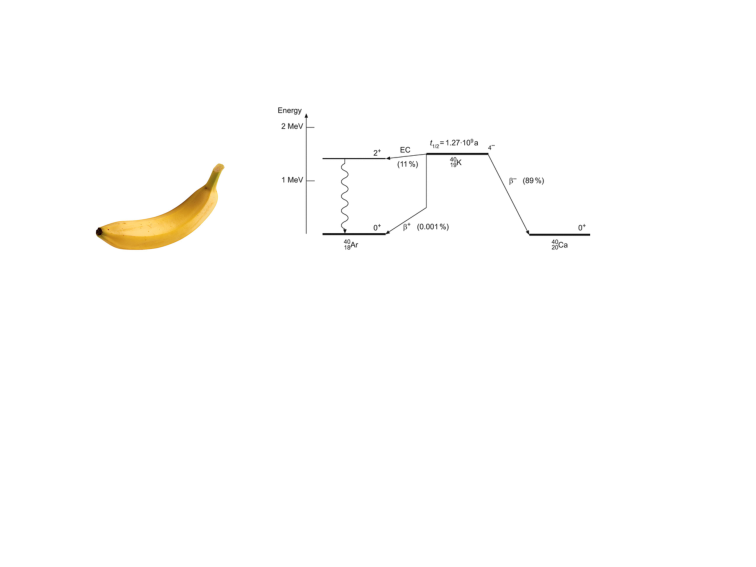
\includegraphics[scale=1.5]{/decadimento_potassio_banane_equivalenti}
\caption{Decadimento del Potassio-40}
\end{figure}

Qual è l'attività di $\SI{1}{g}$ di $K$ naturale?
In un grammo ci sono $N_K = \frac{\SI{1}{g}}{40} \cdot \SI{6.023e23}{} = \SI{1.5e22}{atomi}$ di cui di Potassio-40 
$ N_{^{40}K} = \SI{1.5e22}{} \cdot \SI{1.2e-4}{} = \SI{1.8e18}{atomi} $.
L'attività di $\SI{1}{g}$ di Potassio naturale è pari a
\begin{equation}
A = \frac{dN}{dt} = \lambda N = \frac{\ln 2}{T_{1/2}} = \frac{0.693}{\SI{4e16}{}} = \SI{1.8e18}{} = \SI{31}{Bq}
\end{equation}
in una persona adulta ci sono $\SI{2.5}{g/kg}$ di Potassio, per cui in una persona di $\SI{75}{kg}$ ci sono $\SI{187.5}{g}$ di Potassio e quindi, rispetto al conto precedente, l'attività totale equivale a circa $\SI{5800}{Bq}$.
È da notare che nel corpo umano esistono meccanismi di recupero di questi decadimenti, le cellule sono abituate a recuperare da questo grado di danneggiamento biologico.


\subsubsection{Quantificare danni di eventi disastrosi}
Si quantificano i danni di eventi disastrosi come quelli di Chernobyl facendo una media sulla popolazione.
Noto che una dose di $\SI{1}{Gy}$ è una dose mortale per una persona.
Sapendo la quantità totale di radiazione emessa nell'evento è possibile "dividerla" rispetto alla popolazione per trovarne una media.
Quindi per esempio una dose di $\SI{1}{Gy}$ divisa per $\SI{1000}{persone}$, 1 persona su mille muore per radiazione.

Una dose letale di radiazione espressa in Banane Equivalenti è $\SI{80e6}{BED}$ (lol).

Dormendo a fianco di una persona si è esposti ad una dose di $\SI{0.5}{BED}$.


\subsection{Decadimento $\alpha$}
Nel 1909 Rutherford studia con l'utilizzo di una \emph{camera a nebbia}, uno dei primi rivelatori di particelle, il decadimento nel vuoto di materiale radioattivo e osserva che viene "prodotto" $He$, che osservò come tracce bianche lasciate dal passaggio delle particelle.
Il decadimento $\alpha$ si generalizza come segue
\begin{equation}
\label{decadimento_alpha}
^{A}_{Z}X \quad\rightarrow\quad ^{A-4}_{Z-2}Y + ^{4}_{2}He \quad \Bigl[  + Q  \Bigr]
\end{equation}
in cui il termine $Q$ rappresenta l'energia rilasciata sotto forma di calore.
L'energetica (si chiama così?) del decadimento si calcola, attraverso la solita formula semi-empirica di massa, 
\begin{equation}
Q = M(A,Z) - M(A-4,Z-2) - M_{\alpha}(4,2) = BE(Z-2,A-4) + B_{\alpha} - B(Z,A)
\end{equation}
Se si analizza l'andamento di questa energia in funzione del numero di massa, utilizzando un programma apposito, si trova un andamento del tipo
\begin{figure}[h]
\centering
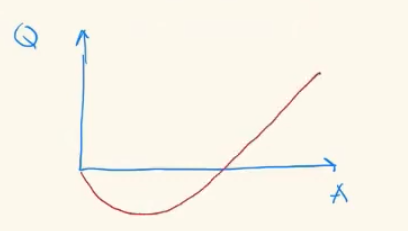
\includegraphics[scale=0.6]{/q_a_alpha}
\caption{CAPTION}
\end{figure}
Il \emph{nucleo di soglia} dal quale il decadimento ha $Q > 0$ corrisponde al numero atomico $A = 150$, quindi gli elementi dal $6^o$ periodo in poi possono decadere $\alpha$, salvo eccezioni come ad esempio l'oro $^{197}_{79}Au$ per il quale nonostante l'energetica sia favorevole al decadimento tale elemento decade con tempi lunghi, più lunghi della vita dell'universo.

\paragraph{Fenomenologia del decadimento alpha} Rappresentando il tempo di decadimento $T_{1/2}$ in funzione dell'energia delle particelle emesse $E_{\alpha}$ si nota una relazione inversa tra le due grandezze, più precisamente data da
\begin{equation}
T_{1/2} \propto \frac{1}{\sqrt{E_{\alpha}}}
\end{equation}
\begin{figure}[h]
\centering
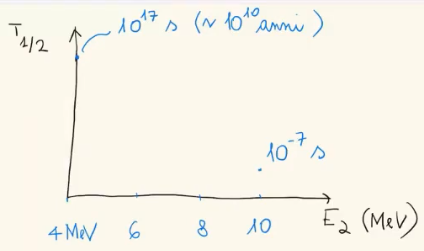
\includegraphics[scale=0.6]{/prop_vitamedia_energiaalpha}
\caption{CAPTION}
\end{figure}
La \emph{legge di Geiger Nuttal} lega la grandezza teorica della \emph{probabilità di decadimento} con le grandezze sperimentalmente misurabili come la \emph{vita media} o il \emph{tempo di dimezzamento}
\begin{equation}
\ln \Bigl(  \frac{1}{\tau}  \Bigr) = a - b \frac{Z}{\sqrt{E_{\alpha}}}
\end{equation}
tale legge ha una validità di $20$ ordini di grandezza, che fa intuire vi siano effetti relativistici che la regolano.

Esistono quattro catene di decadimento alpha molto importanti:
\begin{enumerate}
\item Serie dell'Uranio (o del radio) $^{238}U$ che ha un tempo di vita medio di  $T_{1/2}=\SI{4.5e9}{anni}$ e decade in Piombo $^{206}_{82}Pb$

\item Serie dell'Attino $^{235}U$ che ha un tempo di vita medio di  $T_{1/2}=\SI{7e8}{anni}$ e decade in Piombo $^{207}_{82}Pb$

\item Serie del Torio $^{232}_{90}Th$ che ha un tempo di vita medio di  $T_{1/2}=\SI{1.4e10}{anni}$ e decade in Piombo $^{208}_{82}Pb$

\item Serie del Nettunio $^{237}_{93}Np$ che ha un tempo di vita medio di  $T_{1/2}=\SI{2.2e6}{anni}$ e decade in Bismuto $^{209}_{83}Bi$
\end{enumerate}
Le catene di decadimento vengono utilizzate, tra le altre cose, per le datazioni.
Le precedenti quattro ed il decadimento del Potassio-40 e del Carbonio-14 sono le uniche reazioni di decadimento naturali ancora presenti sulla Terra.
\begin{figure}[h]
\centering
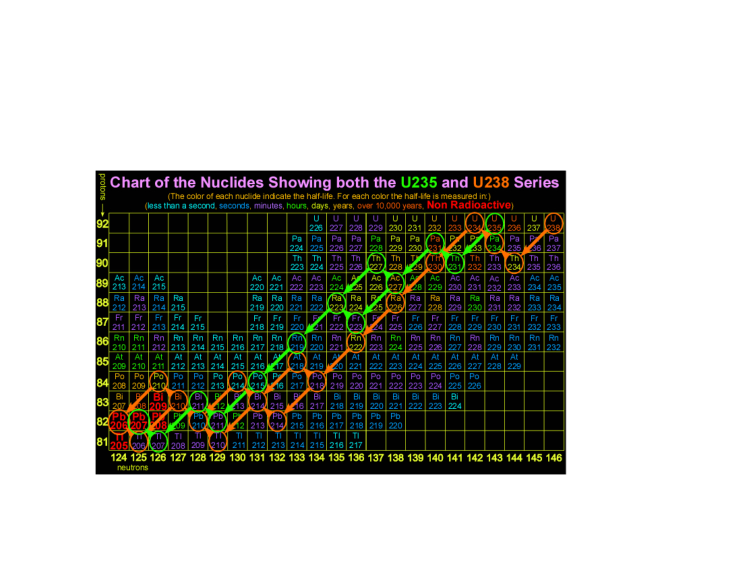
\includegraphics[scale=1.6]{/serie_decadimenti_alpha}
\caption{Serie di decadimenti nucleari dell'Uranio-235 e dell'Uranio-238, in cui si alternano decadimenti $\alpha$ e $\beta$}
\end{figure}

Studiamo il decadimento di un nucleo padre $X$ che decade in un nucleo figlio $Y$ più una particella $\alpha$ ed energia $Q$
\begin{equation}
^{A}_{Z}X \quad\rightarrow\quad ^{A-4}_{Z-2}Y + ^{4}_{2}He + Q
\end{equation}
se inizialmente l'atomo $X$ è a riposo, per la conservazione della quantità di moto, i figli di questa reazione si allontaneranno in direzioni opposte.
La conservazione della quantità di moto si esprime come 
\begin{equation}
p_Y = p_{\alpha} = p
\end{equation}
L'energia liberata nella reazione è divisa tra l'energia cinetica del nucleo figlio e dalla particella $\alpha$, per cui usando la meccanica classica otteniamo
\begin{equation}
Q = \frac{p_Y^2}{2m_Y} + \frac{p_{\alpha}^2}{2m_{\alpha}} 
= \frac{p^2}{2} \Bigl(  \frac{1}{m_Y}  + \frac{1}{m_{\alpha}}\Bigr)
= \frac{p^2}{2} \Bigl(  \frac{m_Y + m_{\alpha}}{m_Y m_{\alpha}} \Bigr)
\end{equation}
da cui si estrae $p^2$
\begin{equation}
p^2 = 2 Q \Bigl(  \frac{m_Y m_{\alpha}}{m_Y + m_{\alpha}} \Bigr)
\end{equation}
da cui si trova come si distribuisce l'energia cinetica nella reazione, l'energia cinetica della particella $\alpha$ è
\begin{equation}
K_{\alpha} = \frac{p^2}{2m_{\alpha}} = Q \frac{m_Y}{m_Y + m_{\alpha}}
\end{equation}
e.g. per un atomo che decade alpha con un numero di massa $A = 200$, sapendo che $A_{\alpha} = 4$ si trova
\begin{equation}
K_{\alpha} = Q \frac{196}{200} \simeq 98\% Q
\end{equation}
e quindi praticamente tutta l'energia cinetica viene trasferita alla particella, mentre solo un $2\%$ dell'energia cinetica viene trasferita all'atomo figlio.
Ha senso quindi approssimare dicendo che l'energia rilasciata nella reazione equivale (circa) all'energia cinetica della particella alpha e quindi si può scrivere $K_{\alpha} = Q$.

\paragraph{nota} se nel decadimento (a due corpi) fosse emesso un elettrone allora l'energia cinetica dell'elettrone sarebbe $K_e = 0.999 Q$

\subsubsection{Cos'è il decadimento $\alpha$}
In un nucleo con massa atomica sufficientemente alta c'è una probabilità non nulla che si formi una particella $\alpha$, un nucleo di Elio, al suo interno, questa particella iniziando a rimbalzare all'interno del nucleo arriverà sulle "pareti".
Il potenziale nucleare è composto da una buca di potenziale che oltre il confine decresce esponenzialmente, l'energia della particella alpha equivale a $E_{\alpha} = \SI{28}{MeV}$.
L'emissione diretta di protoni e neutroni non è possibile in quanto la loro energia $E= 7-\SI{8}{MeV}$ si trova al disotto del livello zero dell'energia e sono intrappolati all'interno.
\begin{figure}[h]
\centering
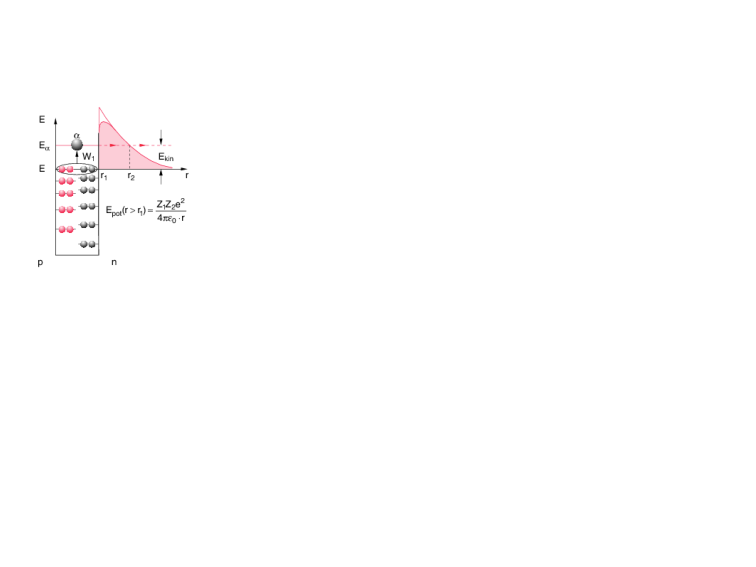
\includegraphics[scale=2]{/alpha_decad_potenziale}
\caption{CAPTION}
\end{figure}
Se i protoni ed i neutroni si combinano insieme in una particella $\alpha$, particella molto stabile, viene emessa un'energia maggiore del livello zero, per cui è inizialmente intrappolata nella buca di potenziale ma ha una probabilità di uscire dalla buca diversa da zero.
Ovviamente solo per effetti quantistici la particella potrà attraversare la regione di potenziale maggiore dell'energia $E_{\alpha}$, classicamente il decadimento $\alpha$ non è possibile o spiegabile.

Cerco qual è la barriera di potenziale che la particella deve superare.
Chiamando $r_1$ la distanza in cui si trova il picco più alto di potenziale, quindi sulla superficie del nucleo, e.g. calcolato per l'Uranio-238 trovo
\begin{equation}
\begin{split}
r_1 & = 1.2 ( 234^{1/3} + 4^{1/3} ) = \SI{9.3}{fm} \\
V_1 & = \frac{ Z_Y \cdot Z_{He} e^2}{4 \pi \varepsilon_0 r_1} = \frac{ 90 \cdot 2 e^2}{4 \pi \varepsilon_0 r_1} = \frac{180 e^2 \hbar c }{4 \pi \varepsilon_0 \hbar c r_1} = \frac{180 \cdot \SI{1.44 }{MeV fm}}{ \SI{9.3}{fm} } =  \SI{27.8}{MeV} 
\end{split}
\end{equation}
La particella $\alpha$ pur avendo energia positiva è inferiore al valore del potenziale, poiché è dell'ordine di qualche $MeV$. 

Cerco ora la distanza che la particella deve percorrere per \emph{effetto tunnel} fino al punto $r_2$ in cui l'energia del potenziale è uguale all'energia della particella $\alpha$.
Per questo conto teniamo ancora in considerazione l'Uranio, l'energia della reazione equivale ad $E_{\alpha} = Q = \SI{4.2}{MeV}$ ed eguagliandolo al potenziale dell'atomo si ricava
\begin{equation}
\begin{split}
& Q = V = \frac{1}{4 \pi \varepsilon_0} \frac{90\cdot2}{r_2} \\
& r_2 = \frac{180 \cdot \SI{1.44}{MeV fm}}{\SI{4.2}{MeV}} = \SI{61.7}{fm}
\end{split}
\end{equation}
La barriera che la particella deve attraversare è molto profonda e non è per questo molto probabile che succeda.


\subsubsection{Teoria di Gamov del decadimento $\alpha$}
La vita media del decadimento è inversamente proporzionale alla probabilità
\begin{equation}
\tau = \frac{1}{\lambda}
\end{equation}
il tempo di decadimento è un parametro fenomenologico, sperimentale, mentre la probabilità di decadimento si ricava dalla teoria.
Secondo la \emph{teoria di Gamov} la probabilità di decadimento è data da tre contributi:
\begin{equation}
\lambda = p_{\alpha} f P
\end{equation}
in cui
\begin{itemize}
\item $p_{\alpha}$ è la \emph{probabilità che si formi una particella $\alpha$}

\item $f$ è la \emph{frequenza di collisione} tra la particella $\alpha$ e gli altri nucleoni nel nucleo ovvero posta $v_{\alpha}]$ la velocità della particella nel nucleo ed $r_1$ la dimensione del nucleo, si ha 
\begin{equation}
\begin{split}
& f = \frac{v_{\alpha}}{2 r_1} \\
& v_{\alpha} = \sqrt{ 2\frac{V_0 + Q}{m_{\alpha}} } \simeq \sqrt{ 2\frac{\SI{35}{MeV} + \SI{5}{MeV}}{\SI{3700}{MeV/c^2}} } \simeq \SI{0.14}{c} = \SI{0.42e8}{m/s}
\end{split}
\end{equation}
considerando ad esempio un nucleo con $A=200$ e raggio $R = \SI{7.0}{fm}$, si trova una frequenza di $f = \SI{6e21}{Hz}$, quindi molto alta

\item mentre il parametro $P$ è legato alla \emph{probabilità di attraversamento della barriera di potenziale}, per il quale è necessario applicare l'equazione di Schrodinger indipendente dal tempo.
Considero il potenziale nella zona 2, in cui decresce da $r_1$ a $r_2$.
Data l'equazione di Schrodinger
\begin{equation}
\begin{split}
& -\frac{\hbar^2}{2m} \frac{d^2 \psi}{dx^2} V \psi = E \psi \quad\Rightarrow\quad 
\frac{d^2\psi}{dx^2} = - \frac{2m}{\hbar^2} (E-V)\psi = -\frac{2m}{\hbar^2} (Q-V_c)\psi \\
& K^2 =  -\frac{2m}{\hbar^2} (Q-V_c) \quad > 0 \\
&  \frac{d^2\psi}{dx^2} = K^2 \psi \quad\Rightarrow\quad \psi = \cancel{A e^{+ K x}} + Be^{- K x}
\end{split}
\end{equation}
si trova la funzione d'onda $\psi$ che descrive la particella nella zona classicamente proibita.
Il termine $P$


\end{itemize}

















\section{Fissione e Fusione Nucleare}

%Zarantonello Umberto 2021-05-24

\section{Acceleratori di Particelle}

%nuova sezione----------------------------------------------------------------------------- 
\subsection{Fisica degli acceleratori di particelle}
La conoscenza della fisica degli acceleratori è essenziale per ogni tipo di fisico in quanto ha applicazioni in ogni campo fisico.
Ne approfondiamo quindi quelli che sono i fondamenti e le grandezze base per poter avere un'idea più chiara del loro funzionamento.

Per capire la grande applicabilità di questi strumenti, attualmente al mondo sono attivi $15000$ acceleratori di cui: $8500$ con applicazioni industriali, $5500$ con applicazioni mediche e $1000$ con applicazioni in ricerca (di cui $100$ usati per la fisica nucleare e subnucleare).
L'attenzione mondiale alla fisica nucleare cambiò radicalmente prima e dopo la seconda guerra mondiale e anche gli acceleratori sono figli dell'aumento dell'interesse a questi ambiti.
Già a Rutherford dopo i suoi studi era chiaro che l'accelerazione di particelle sarebbe stato il passo successivo per la scoperta e l'approfondimento di questa nuova fisica.
Solo avendo il controllo della quantità ed energia di particelle si sarebbe potuto infatti ottenere una maggiore risoluzione nello studio del nucleo.

I parametri che caratterizzano gli acceleratori sono sostanzialmente l'energia e la luminosità.

\paragraph{Energia}

\'E importante conoscere l'energia perché la risoluzione con la quale possiamo risolvere un bersaglio dipende dalla lunghezza d'onda della sonda con la quale bombardiamo l'oggetto in analisi.
Prendendo un oggetto di raggio R, la lunghezza d'onda della sonda dovrà essere
\begin{equation}
\begin{split}
\lambda=\frac{h}{p}&<2R\\
2\pi \frac{\hbar c}{pc}&<2R
\end{split}
\end{equation}
Vuol dire che se vogliamo risolvere una struttura di dimensione $2R$ dobbiamo avere un fascio di energia
\begin{equation}
pc\simeq E>2\pi\frac{\hbar c}{2R}
\end{equation}
Inserendo quindi un po' di dimensioni, se vogliamo per esempio studiare il protone ($r=1fm$) serve un energia pari a 
\begin{equation}
E=pc=600MeV
\end{equation}
Se per esempio invece volessimo studiare i quark($r=10^{-4}fm$) allora l'energia sarà
\begin{equation}
E\simeq 6TeV
\end{equation}

Un altro motivo per cui è essenziale l'energia negli acceleratori deriva dalla famosa formula di Einstein
\begin{equation}
E=mc^2
\end{equation}
Che prevede la convertibilità tra massa ed energia.
Nella sezione precedente abbiamo infatti visto come sia possibile generare energia trasformando della massa.
Se questo è vero allora sarà vero anche il contrario, infatti è stato visto negli acceleratori che da scontri tra particelle altamente energetiche è possibile generare nuove particelle.
Per cui un grande utilizzo di questi apparati deriva proprio dalla necessità di generare particelle che sono state crucciali nello studio dell'evoluzione dell'universo che però sono ormai decadute per il basso tempo di decadimento.
Per dire proprio a questo scopo è stato costruito l'LHCb del Cern.

\paragraph{Metodi di collisione}
Esistono due modi per studiare le collisioni tra particelle: il metodo con il collisore e la collisione su bersaglio fisso.
Nel caso di collider (metodo del collisore) si sfruttano due fasci il che porta a delle energie nel centro di massa molto elevate (è quindi adatto alla produzione di nuove particelle).
Nel caso invece del bersaglio fisso l'energia è più bassa, ergo si fa più fatica a produrre nuove particelle, è favorita però la \emph{luminosità}.

Facciamo quindi delle stime sui due metodi
\begin{itemize}
\item \emph{Caso del collisore simmetrico}

Si consideri di avere due fasci paralleli e opposti in collisione, per semplicità adotteremo la semplificazione $\hbar=c=1$.
Il quadrivettore legato alla particella 1 è dato da
\begin{equation}
p_1^*=(E_1^*,\bar{p})
\end{equation}
(con asterisco indico le quantità misurate nel centro di massa).
Siccome i due fasci hanno lo stesso momento contropropagante è utile porsi nel sistema di riferimento del centro di massa , inoltre le due quantità di moto saranno identiche per cui non serve distinguere tra $\bar{p_1}$ e $\bar{p_2}$.
\begin{equation}
p_2^*=(E_2^*,-\bar{p})
\end{equation}
Si sa dalla meccanica relativistica che il quadrato del quadrivettore è un invariante relativistico
\begin{equation}
{p_1^*}^2=E_1^*-\bar{p}^2=m_1^2\hspace{0.5cm}{p_2^*}^2=E_2^*-\bar{p}^2=m_2^2
\end{equation}
L'energia nel centro di massa è la somma dei quadrivettori al quadrato
\begin{equation}
\begin{split}
s=(p_1^*+p_2^*)2&=(E_1^*+E_2^*, \bar{p}-\bar{p})^2\\
\to E_{CM}=\sqrt{s}&=E_1^*+E_2^*
\end{split}
\end{equation}
Suppongo che il collider è simmetrico e che le particelle scontrate siano in entrambi i casi protoni (quindi di massa $m_p$).
L'energia di ogni fascio sarà
\begin{equation}
E_1*=m_1+T_{cm}=m_p+T_{cm}
\end{equation}
L'energia invece del centro di massa corrisponde a 
\begin{equation}
\sqrt{s}=E_{cm}=2m_p+2T_{cm}
\end{equation}
Quello che ci interessa è che se suppongo che l'energia nel centro di massa sia molto maggiore della massa del protone ($T_{cm}\gg m_p$), ottengo
\begin{equation}
T_{cm}=\frac{\sqrt{s}}{2}\to \sqrt{s}=2T_{cm}
\end{equation}
Quello che ci interessa è che in un collider l'energia nel centro di massa è linearmente dipendente dall'energia cinetica nel centro di massa.
Questo è importante perché quello che voglio creare nel centro di massa sono nuove particelle e così posso controllarne l'energia.

Il collider è un concetto molto complicato in quanto non è banale far scontrare due fasci, bisogna considerare che le dimensioni dei fasci infatti sono dell'ordine del millimetro e l'acceleratore è spesso lungo centinaia di metri.

Supponiamo di far scontrare due protoni e di voler creare un pione, particella costituita da un quark ed un anti quark.
\begin{equation}
pp\to pp\pi^0
\end{equation}
La massa di un pione è di 
\begin{equation}
m_{\pi^0}\simeq 130MeV/c^2
\end{equation}
L'energia dei due fasci per la formazione di un pione deve essere uguale a 
\begin{equation}
s_{cm}=(2m_pmm_{\pi^0})^2
\end{equation}
L'energia cinetica delle particelle deve soddisfare la condizione
\begin{equation}
2m_p+2T_{cm}\ge 2m_p+m_{\pi^0}
\end{equation}
e quindi essere
\begin{equation}
T_{cm}\ge \frac{m_{\pi^0}}{2}=67,5MeV
\end{equation}
L'energia cinetica richiesta per ogni fascio sarà quindi sempre pari alla metà dell'energia di massa della singola particella.
Questo si ottiene in quanto dobbiamo considerare che il centro di massa sarà sempre uguale.

\item \emph{Caso del bersaglio fisso}

Nel sistema di riferimento del laboratorio abbiamo che i due quadrivettori saranno 
\begin{equation}
\begin{split}
p_1&=(E_1,\bar{p_1}\\
p_2&=(m_2,0)
\end{split}
\end{equation}
Nel centro di massa il quadrivettore energia è 
\begin{equation}
\begin{split}
s&=[(E_1+m_2)^2-(\bar{p_2}+0)^2]\\
&=E_1^2+2E_1m_2+m_2^2-\bar{p_1}^2\\
&=m_1^2-+m_2^2+2E_1m_2
\end{split}
\end{equation}
A questo punto faccio le stesse considerazioni del collider, suppongo che le due particelle coincidano ($m_1=m_2=m_p$) e che l'energia della prima particella sia
\begin{equation}
E_1=m_1+T^{lab}
\end{equation}
ottengo quindi 
\begin{equation}
\begin{split}
s & =m_p^2 + m_p^2 + 2(m_p+T^{lab})m_p\\
\sqrt{s}&=\sqrt{4m_p^2+2T^{lab}m_p}
\end{split}
\end{equation}
Se mi pongo nella condizione in cui $T^{lab}\gg m_p$ ottengo
\begin{equation}
\sqrt{s}=\sqrt{2m_pT^{lab}}
\end{equation}

La differenza con il caso precedente è immediata, in un esperimento a bersaglio fisso l'energia nel centro di massa cresce linearmente con $\sqrt{T^{lab}}$.
Se volessi creare un pione con questa configurazione dovrei richiedere un'energia di soglia
\begin{equation}
\begin{split}
T^{lab}_{Th}&=\frac{s_{Th}-4m_p^2}{2m_p}\\
s_{Th}&=(2m_p+2m_{\pi^0})^2\\
T^{lab}_{Th}&=\frac{(2m_p+2m_{\pi^0})^2-4m_p^2}{2m_p}=280MeV
\end{split}
\end{equation}
Questo è solo un esempio per capire la differenza tra i due tipi di acceleratore.
\end{itemize}

\paragraph{Luminosità}
La luminosità $L$ corrisponde al numero di eventi (collisioni) per unità di area al secondo, è una grandezza importante perché se voglio calcolare il rate di eventi di un certo tipo 
\begin{equation}
R=\sigma L
\end{equation}
dove $\sigma$ è la sezione d'urto.

Per esempio nel Lep, che è stata la macchina progenitrice dell'LHC (funzionante tramite leptoni) e con cui si è studiato il modello standard, la produzione di coppie $W^+, W^-$ era di $\sigma=15pb$ e la luminosità (che si misura in numero di particelle su centimetro quadro al secondo) era di $L=10^{32}\cdot/cm^2s$.
Il che restituiva un rate di coppie pari a 
\begin{equation}
\frac{dW^+W^-}{dt}=15\times 10^{-12}\times 10^{-28}m^2\cdot 10^{32}\frac{1}{cm^2s}=1,5\times 10^{-3}\frac{eventi}{s}
\end{equation}
Si verificavano quindi un paio di eventi ogni ora.

La luminosità integrata nel tempo è una quantità che serve per capire per quanto tempo ho la necessità di sfruttare una strumentazione
\begin{equation}
L=\int Ldt
\end{equation}

La luminosità nel caso del collider si calcola come
\begin{equation}
L=\frac{nfN_1N_2}{A}
\end{equation}
dove $n$ è il numero di bunches (le particelle solitamente non sono distribuite uniformemente nei fasci a causa dei metodi sfruttati per collimare i fasci, vengono invece distribuite in pacchetti), $N_1, N_2$ sono il numero di particelle per bunch (ce ne sono due perché abbiamo due fasci e non sempre sono fasci uguali), $f$ è la frequenza di rivoluzione e $A$ è la sezione del fascio.
\'E intuitivo che per aumentare la luminosità dobbiamo rendere il fascio più piccolo possibile.

Nel caso del bersaglio fisso la luminosità è data da
\begin{equation}
L=\Phi_a N_b
\end{equation}
dove $\Phi_a$ è l'intensità di particelle del fascio e $N_b$ è il numero di particelle nel bersaglio.
L'intensità di particelle del fascio è uguale al numero di particelle al secondo diviso l'area
\begin{equation}
\Phi_a=\frac{N_a(s)}{A}
\end{equation}
che può anche essere scritta come la densità di particelle per unità di volume per la velocità delle particelle stesse
\begin{equation}
L=n_a v_a
\end{equation}
Mentre il numero di particelle del bersaglio è uguale alla densità delle particelle del bersaglio per lo spessore per l'area interessata del fascio
\begin{equation}
N_b=n_bd\cdot A
\end{equation}
La luminosità è quindi riscrivibile come
\begin{equation}
L=N_an_bd=n_av_aN_b
\end{equation}

%nuova sezione-----------------------------------------------------------------------------
\subsection{Tipi di Acceleratore}
Gli acceleratori si possono suddividere in due grandi categorie: acceleratori lineari e circolari.
\paragraph{Acceleratori Lineari}
Sono acceleratori elettrostatici ossia in questi acceleratori l'accelerazione avviene tramite una differenza di potenziale elettrostatico. 
In questa categoria sono inclusi gli acceleratori: 
\begin{itemize}
\item Van de Graaf
\item Cockrof-Walton
\item Tandem
\item il LINAC.
\end{itemize}
Il limite di questi acceleratori sta nel fatto che utilizzano un'unica differenza di potenziale, il che pone un limite a ciò che si può creare infatti le differenze di potenziale sono limitate dalla rottura del dielettrico.
Sono i primi che sono stati utilizzati e i massimi campi che si riesce a creare nel vuoto sono di $6-7MeV/m$

\paragraph{Acceleratori circolari}
Questi acceleratori ovviano al limite della differenza di potenziale facendo passare la particella più volte per la stessa differenza di potenziale facendo bastare così una piccola differenza di potenziale ben posta.
Di questi fanno parte:
\begin{itemize}
\item ciclotrone
\item betatrone
\item sincrotrone
\end{itemize}

\subsubsection{Van De Graaf}
\begin{figure}[h]
\centering 
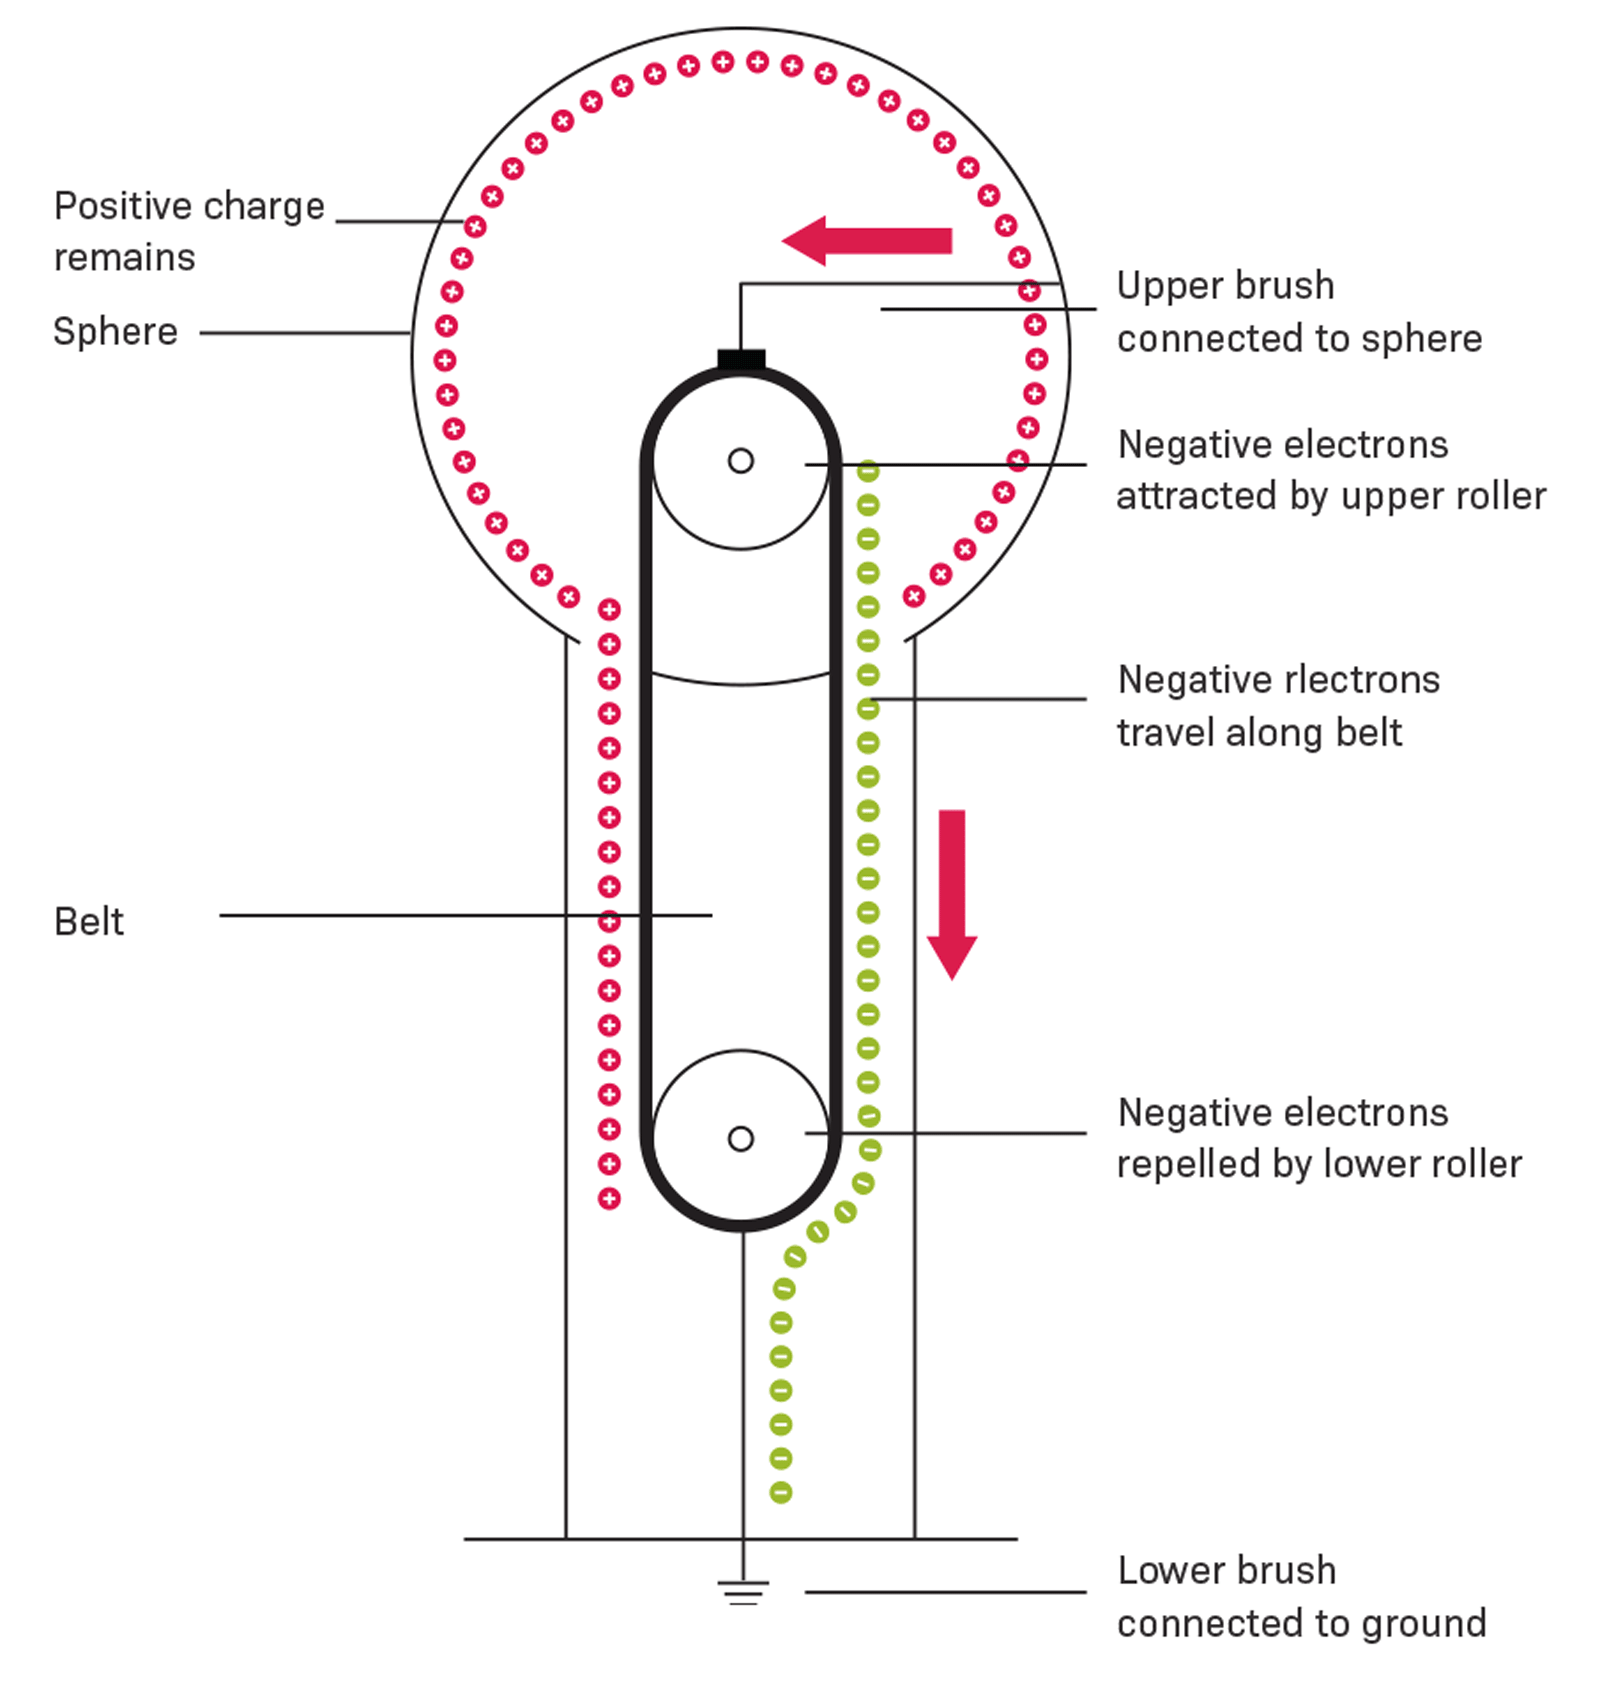
\includegraphics[width=160pt]{fig7_01}
\caption{Schema di un acceleratore di van de Graaf}
\end{figure}
L'acceleratore di Van De Graaf si compone come in figura.
La struttura è formata da una cinghia che scorre e si carica grazie a delle punte per scorrimento.
La cinghia poi passa per una sfera cava su cui viene trasferita la carica che, per i principi dell'elettrodinamica, si va a distribuire su tuttala superficie.
In questo modo si riescono a creare una differenza di potenziale dell'ordine di qualche $MeV$.
Tutto il sistema viene messo all'interno di grossi contenitori isolati in quanto l'aria farebbe scaricare le superfici (i gas inerti sostitutivi sono solitamente $SF_6, N_2+CO_2$).

Il \textbf{Tandem}, è basato sullo stesso principio del Van de Graaf, solo che la differenza di potenziale viene raddoppiata, ponendo la sfera all'interno di un altro conduttore.
\begin{figure}[h]
\centering
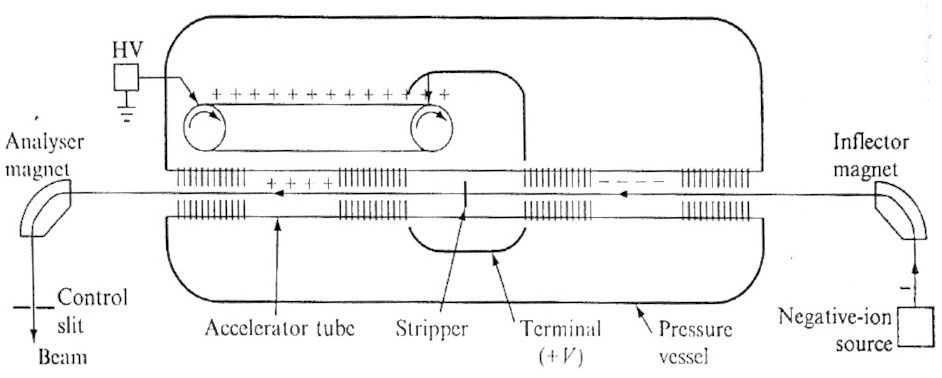
\includegraphics[width=250pt]{fig7_02}
\caption{Configurazone Tandem}
\end{figure}
Il potenziale che si riesce a creare è il doppio del potenziale di partenza.
A Legnaro è presente un acceleratore con questa configurazione e viene utilizzato per esperimenti di \emph{Rutherford backscattering}, in cui si sfrutta lo scattering del fisico neozelandese per esperimenti di spettroscopia (studiando l'energia delle particelle backscatterate si riesce a capire la composizione superficiale del bersaglio).

\subsubsection{Acceleratore lineare: LINAC}
Il LINAC è stato rivoluzionario come acceleratore perché supera il limite nella generazione di potenziali.
Questo acceleratore è composto da una serie di elettrodi separati che variano la polarità con un'onda a radiofrequenza.
\begin{figure}[h]
\centering
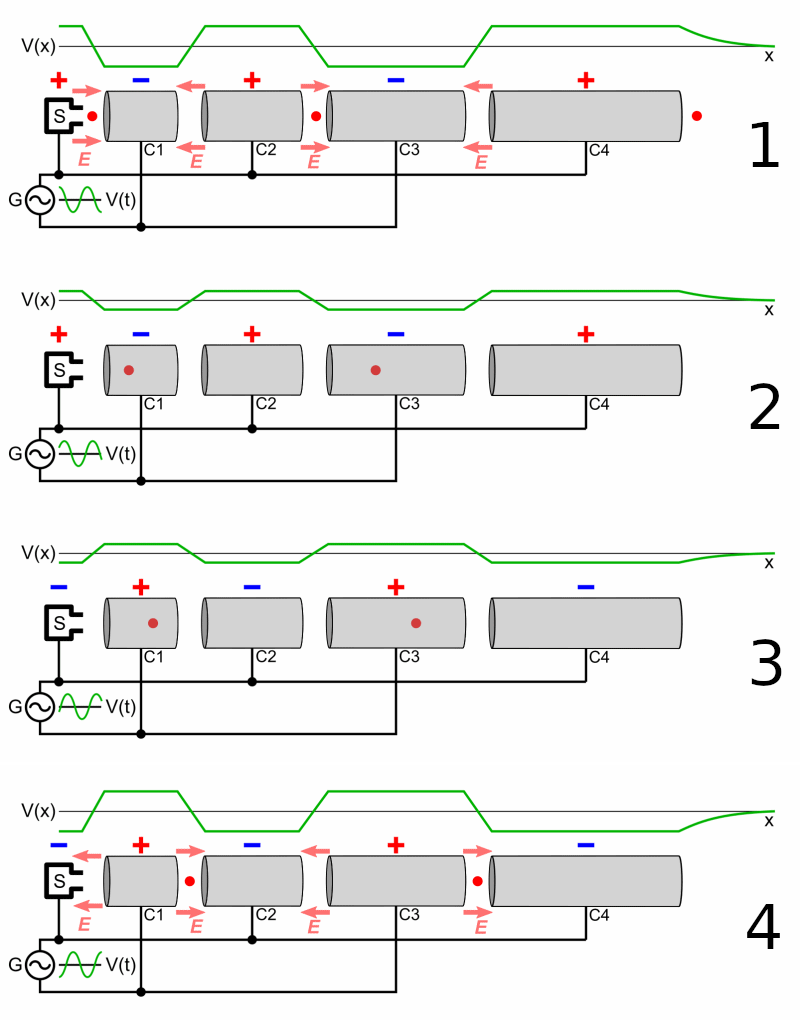
\includegraphics[width=180pt]{fig7_03}
\caption{Schema di funzionamento di un acceleratore lineare}
\end{figure}

Quello che si vuole generare con questo tipo di configurazione è un potenziale sempre negativo per la particella accelerata, infatti riuscendo a variare il potenziale al passaggio della particella, facendolo passare da positivo a negativo e viceversa, la particella nel sistema sarà sempre accelerata da un potenziale negativo rispetto a quello che ha alle sue spalle (che nel frattempo è diventato positivo).
Tutto questo fa si che pur mantenendo una differenza di potenziale piuttosto bassa si riesca ad accelerare particelle ad alte energie, questo metodo è usato per esempio per gli elettroni (in orbita circolare gli elettroni emettono radiazione).

\subsubsection{Ciclotrone}
Il ciclotrone utilizza una combinazione di campi elettrici e magnetici.
Supponiamo di avere un campo magnetico entrante e di porci una particella (per esempio un protone) ciò che si crea è una forza di Lorentz, quindi a causa del campo magnetico la particella percorre una traiettoria circolare.
\begin{figure}[h]
\centering
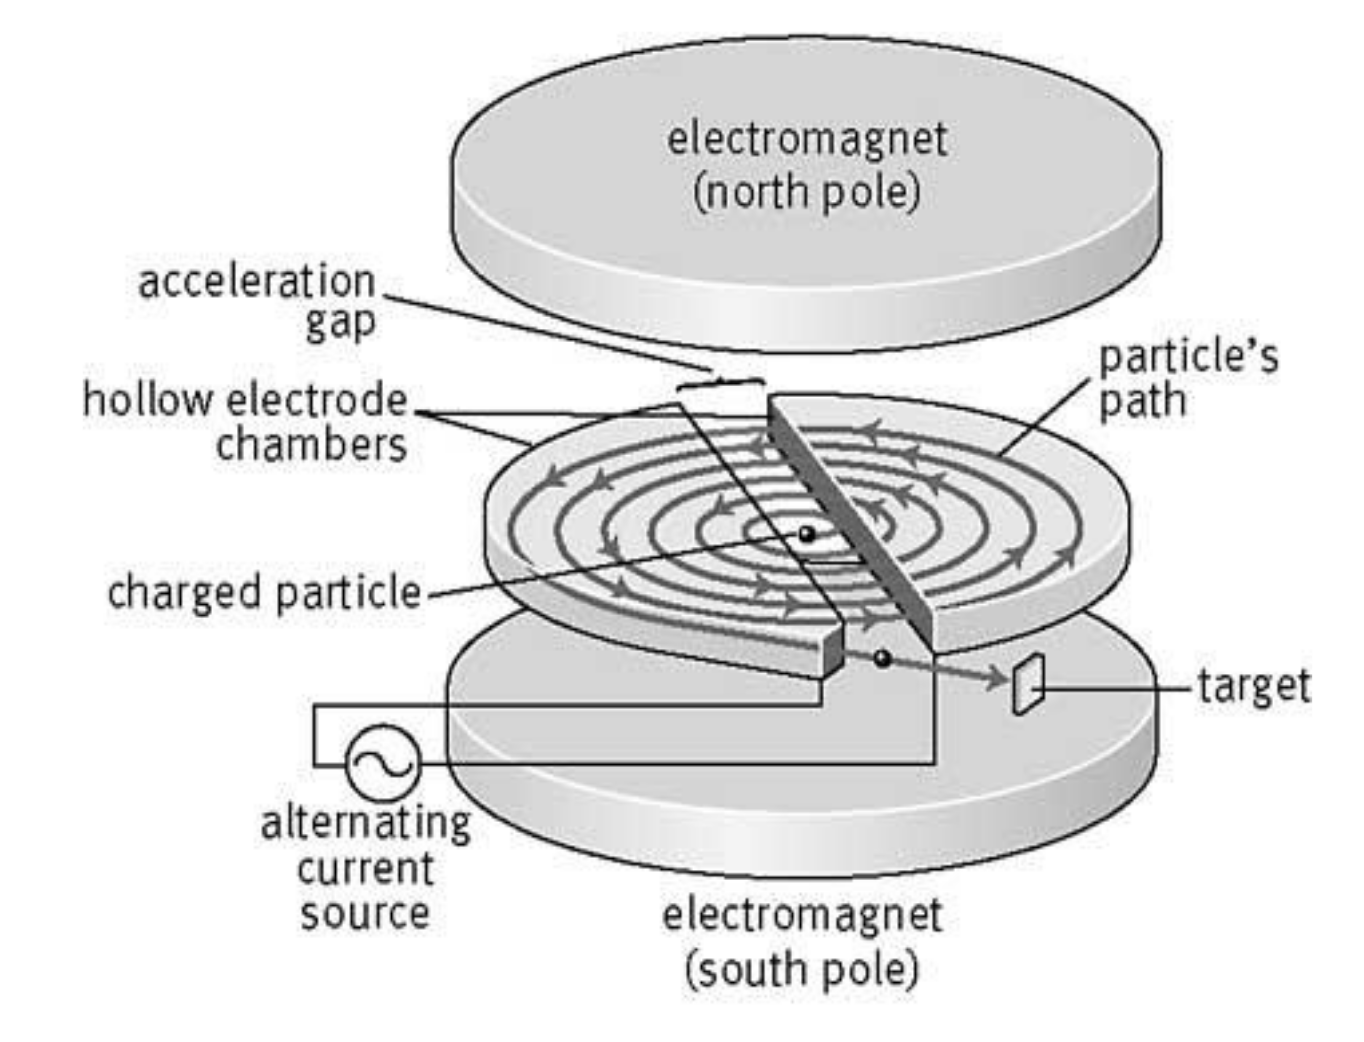
\includegraphics[width=150pt]{fig7_04}
\caption{Struttura del ciclotrone}
\end{figure}

All'interno di una situazione in cui due elettrodi hanno forma a D e sono immersi all'interno di un campo magnetico, questi vengono polarizzati uno con polarità positiva e uno con polarità negativa.
Se non si fa nulla il protone passa dal $+$ al $-$ e se cambio a polarità fa il percorso inverso.
Siccome voglio confinare la particella  applico un campo magnetico ortogonale al piano degli elettrodi.
La combinazione di campo magnetico e cambio di polarità genera un moto circolare del protone che ad ogni passaggio viene accelerato.
In questo modo si riesce ad aumentare la velocità delle particelle fino a che non raggiunge la velocità desiderata e allora posso estrarlo.

Calcoliamo le leggi che agiscono sulla particella.
Innanzitutto si ha la forza di Lorentz
\begin{equation}
F=Bqv
\end{equation}
Che corrisponde alla forza centripeta
\begin{equation}
Bqv=m\frac{v^2}{r}\to v=\frac{Bqr}{m}
\end{equation}
Calcoliamo la frequenza di variazione del campo elettrico per mantenere la particella in moto.
Il periodo di rotazione della particella è
\begin{equation}
T=\frac{2\pi r}{v}=\frac{2\pi r}{\frac{Bqr}{m}}=\frac{2\pi m}{Bq}
\end{equation}
Quindi la frequenza con cui devo variare i due elettrodi sarà
\begin{equation}
f=\frac{Bq}{2\pi m}
\end{equation}
\'E interessante notare come questa non dipenda dal raggio perché a mano a mano che la velocità aumenta la particella percorre percorsi maggiori e quindi queste due quantità si compensano.
Questo è ovviamente valido finché non si manifestano effetti relativistici sulla massa
\begin{equation}
m=m_0\cdot \gamma
\end{equation}
Esiste quindi un limite che corrisponde a qualche percentuale della velocità della luce (per esempio un protone che ha massa dell'ordine del $GeV$ può essere accelerato fino ad un massimo di $\sim 20MeV$).

\subsubsection{Betatrone}
\'E anche questo un acceleratore circolare.
Il campo magnetico viene usato in questo caso sia per il confinamento che per l'accelerazione delle particelle.
Se è vero che il campo magnetico di per sé non può accelerare le particelle si sa anche che la variazione del campo, grazie alla legge di Faraday, genera un campo elettrico.
La configurazione magnetica del Betatrone viene mostrata in figura ed è formata da due piastre conduttrici a forma di piatto rovesciato separate da una ciambella ceramica.
\begin{figure}[h]
\centering
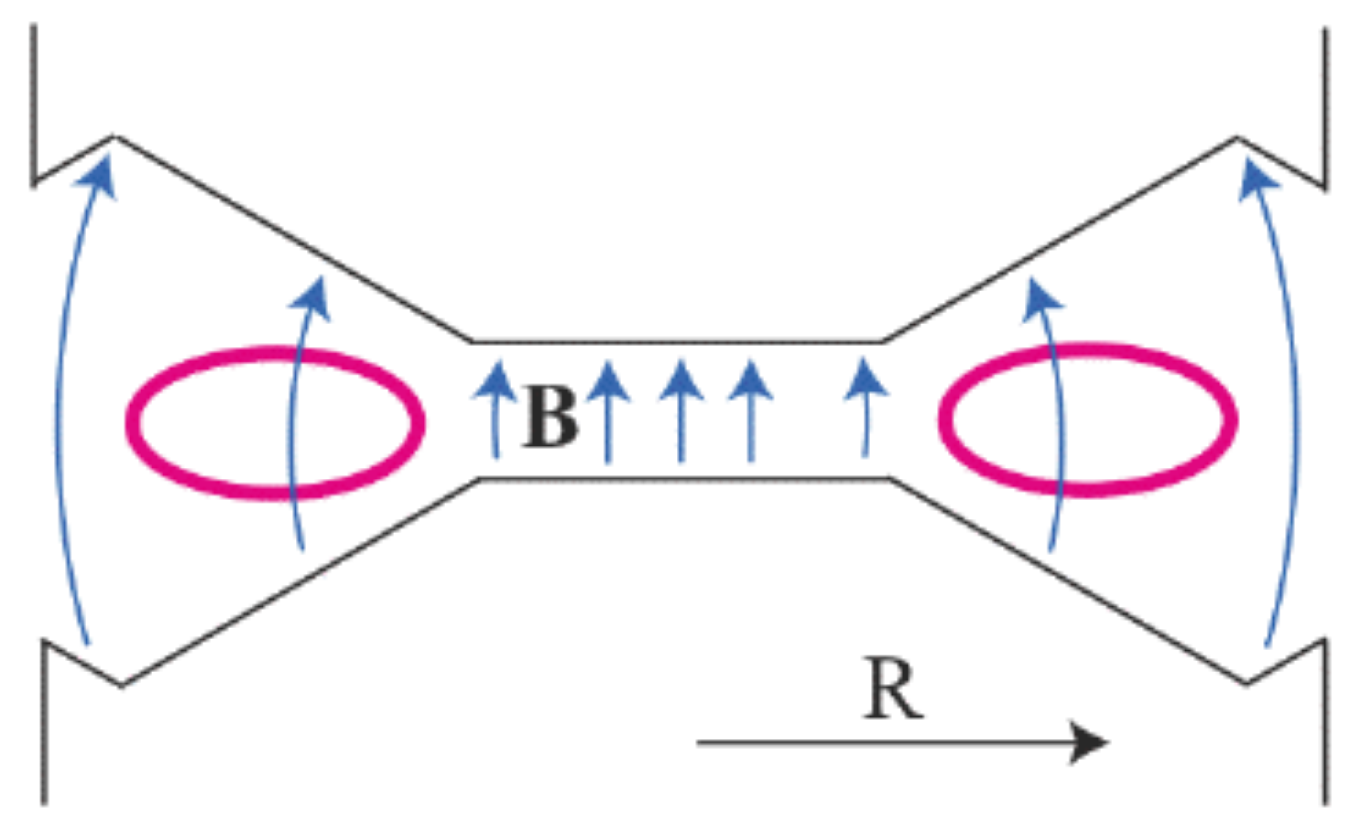
\includegraphics[width=150pt]{fig7_05}
\caption{Sezione verticale del Betatrone}
\end{figure}

Il campo magnetico è costante nel centro della configurazione ma decresce andando verso l'esterno.
La ciambella ceramica  è vuota ed è il percorso all'interno del quale vengono accelerate le particelle.
Il fatto che il campo decresca genera un problema di focalizzazione, per questo viene solitamente considerato un sistema a focalizzazione debole.
Bisogna considerare che le particelle continuando a percorrere più volte lo stesso spazio tenderanno ad avere traiettorie leggermente diverse e quindi un po' alla volta si disperderanno.

Ci concentriamo ora sui campi.
Chiamiamo $\bar{B}$ il campo magnetico medio interno alla ciambella e $B_0$ il campo che le particelle vedono.
Se varia il campo medio viene generato un campo elettrico che è quello che porta all'accelerazione delle particelle mentre $B_0$ corrisponde al campo che tiene le particelle all'interno della cavità, ci deve essere quindi una ben definita relazione tra $\bar{B}$ e $B_0$.

La prima legge che ci è utile è la legge di Faraday-Lenz
\begin{equation}
\frac{d\Phi (B)}{dt}=-\oint \vec{E} d\vec{l}
\end{equation}
Sfruttando la legge di Faraday-Lenz è possibile trovare il campo elettrico corrispondente al flusso magnetico
\begin{equation}
\pi R^2\frac{d\bar{B}}{dt}=-E2\pi R \to E=-\frac{R}{2}\frac{d\bar{B}}{dt}
\end{equation}
dove $R$ è il raggio totale della ciambella.
La forza che accelera le particelle corrisponde quindi a 
\begin{equation}
F=-eE=\frac{eR}{2}\frac{d\bar{B}}{dt}
\end{equation}
Allo stesso tempo il campo $B_0$ deve fornire l'accelerazione centripeta per tenere le particelle all'interno della cavità.
\begin{equation}
evB_0=\frac{mv^2}{R}\to \frac{pv}{R}evB_0\to p=eRB_0
\end{equation}
Ricaviamo quindi anche la forza necessaria al campo $B_0$
\begin{equation}
F=\frac{dp}{dt}=\frac{d}{dt}(erB_0)=eR\frac{dB_0}{dt}
\end{equation}
Ora per ottenere un moto circolare costante è necessario eguagliare le due forze
\begin{equation}
\frac{eR}{2}\frac{d\bar{B}}{dt}=eR\frac{dB_0}{dt}\to \frac{dB_0}{dt}=\frac{1}{2}\frac{d\bar{B}}{dt}
\end{equation}
Integrando si ricava dunque la condizione 
\begin{equation}
\bar{B}=2B_0+cost
\end{equation}

\subsubsection{Sincrotrone}
\'E un acceleratore circolare a sfrutta anch'esso i campi magnetici (sono l'unico modo per accelerare delle particelle) e la cui idea di base è il disaccoppiamento delle funzioni principali dell'acceleratore.
\begin{figure}[h]
\centering
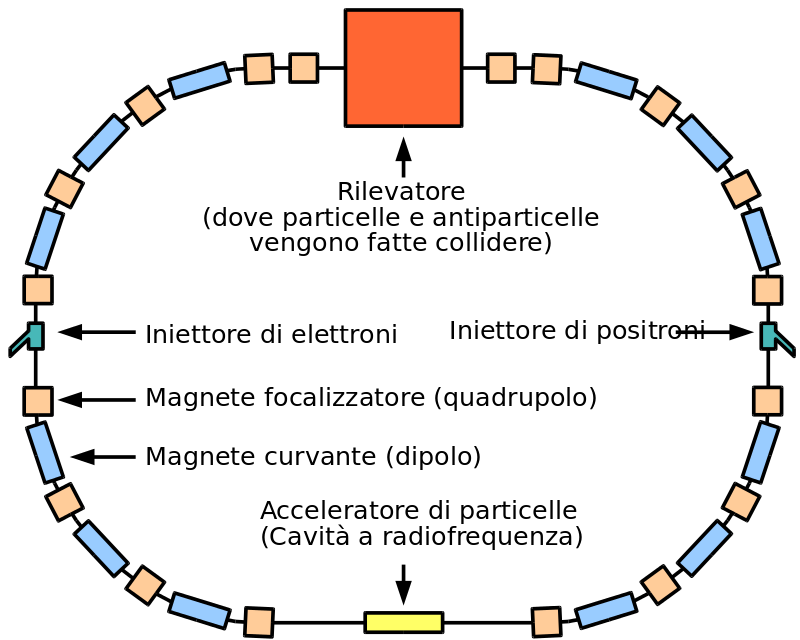
\includegraphics[width=190pt]{fig7_06}
\end{figure}

Il campo magnetico in questo caso viene generato da quella che viene chiamata cavità a radiofrequenza, ovvero un qualunque dispositivo con all'interno un campo elettrico oscillante con la frequenza delle radio-onde.
In questa cavità la particella passerà con una certa frequenza e il modo per accelerarla è fare si che ad ogni passaggio sia sempre in una fase del campo elettrico accelerante.
Bisogna considerare che all'interno del sincrotrone la particella avrà una frequenza dell'ordine del $MHz$ (ogni secondo le particelle faranno un milione di giri all'interno dell'anello di accumulazione) e che per fare esperimenti l'obiettivo è di tenere le particelle per ore all'interno del dispositivo, per cui il minimo errore di traiettoria provocherebbe la dispersione del fascio.
 
Le grandezze di base (e indipendenti tra loro) del sincrotrone sono:
\begin{itemize}
\item \emph{Accelerazione}: tramite campi elettrici a radiofrequenza;

\item \emph{Guida}: tramite dipoli magnetici;

\item\emph{Focalizzazione}: tramite quadrupoli magnetici.
\end{itemize}
L'accelerazione non verrà trattata per tempistiche, studiamo però i campi magnetici che vengono sfruttati.

Il \emph{campo di dipolo magnetico} è composto da due poli, uno nord e uno sud, con le linee di campo dirette da nord a sud perpendicolarmente.
\begin{figure}[h]
\centering
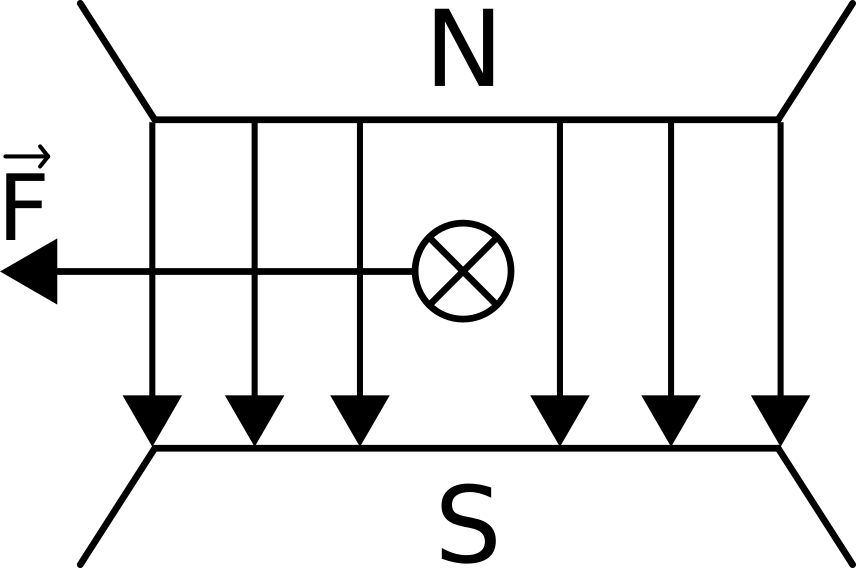
\includegraphics[width=140pt]{fig7_07}
\end{figure}

Supponendo di avere una carica positiva entrante nel dipolo, per la regola della mano destra viene generata una forza perpendicolare sia al campo che alla particella.
In questo modo il dipolo confina la particella senza compiere lavoro (i campi magnetici non compiono mai lavoro), generando un moto circolare.
Calcoliamo quindi la relazione tra la curvatura e il campo magnetico sfruttando la relazione di Lorentz.
\begin{equation}
\begin{split}
\frac{mv^2}{R} & =qvB\\
mv & =qRB\\
p & =qRB\\
pc & =qcRB
\end{split}
\end{equation}
Nel sistema di unità di misura internazionale $pc$ si misura in $[J]$, $B$ in $[T]$ e il raggio $R$ in $[m]$.
\begin{equation}
pc[J]=1,6\times10^{-19}C\cdot3\times10^8\frac{m}{s}B[T]R[m]
\end{equation}
Volendo però passare alle unità naturali si ottiene
\begin{equation}
pc [GeV]=0,3 B[T]R[m]
\end{equation}
$B\cdot R$ viene solitamente chiamata rigidità magnetica dell'anello.

Questa formula è molto utile perché, conoscendo direttamente il campo magnetico e la lunghezza di un anello, possiamo già calcolare l'energia massima a cui possiamo accelerare le particelle.
Per esempio l'LHC del Cern ha un raggio di 
\begin{equation}
2\pi R=27km
\end{equation}
E un campo medio esistente di 
\begin{equation}
B=5,4T
\end{equation}
Il che porta a particelle di quantità di moto
\begin{equation}
p=7\frac{TeV}{c}
\end{equation}
Il numero di dipoli che devo inserire poi in un anello è di 
\begin{equation}
\theta=\frac{2\pi}{N}
\end{equation}
Dove $N$ è il numero di dipoli.
Un'altra cosa che posso già calcolare, sapendo $\theta$ e la lunghezza di un dipolo $L$ è il raggio di curvatura
\begin{equation}
R=\frac{L}{\theta}
\end{equation}

Ora abbiamo visto il confinamento delle particelle e il suo funzionamento ma c'è da considerare che la vita media delle particele in un sincrotrone è di una decina di ore e che la mole di particelle è dell'ordine del miliardo è quindi fondamentale la \emph{focalizzazione}.
Come abbiamo visto il metodo di focalizzazione è il \emph{quadrupolo magnetico}, composto, come suggerisce il nome, da quattro poli, due nord e due sud.
Le linee di campo anche in questo caso sono rivolte da nord a sud.
\begin{figure}[h]
\centering
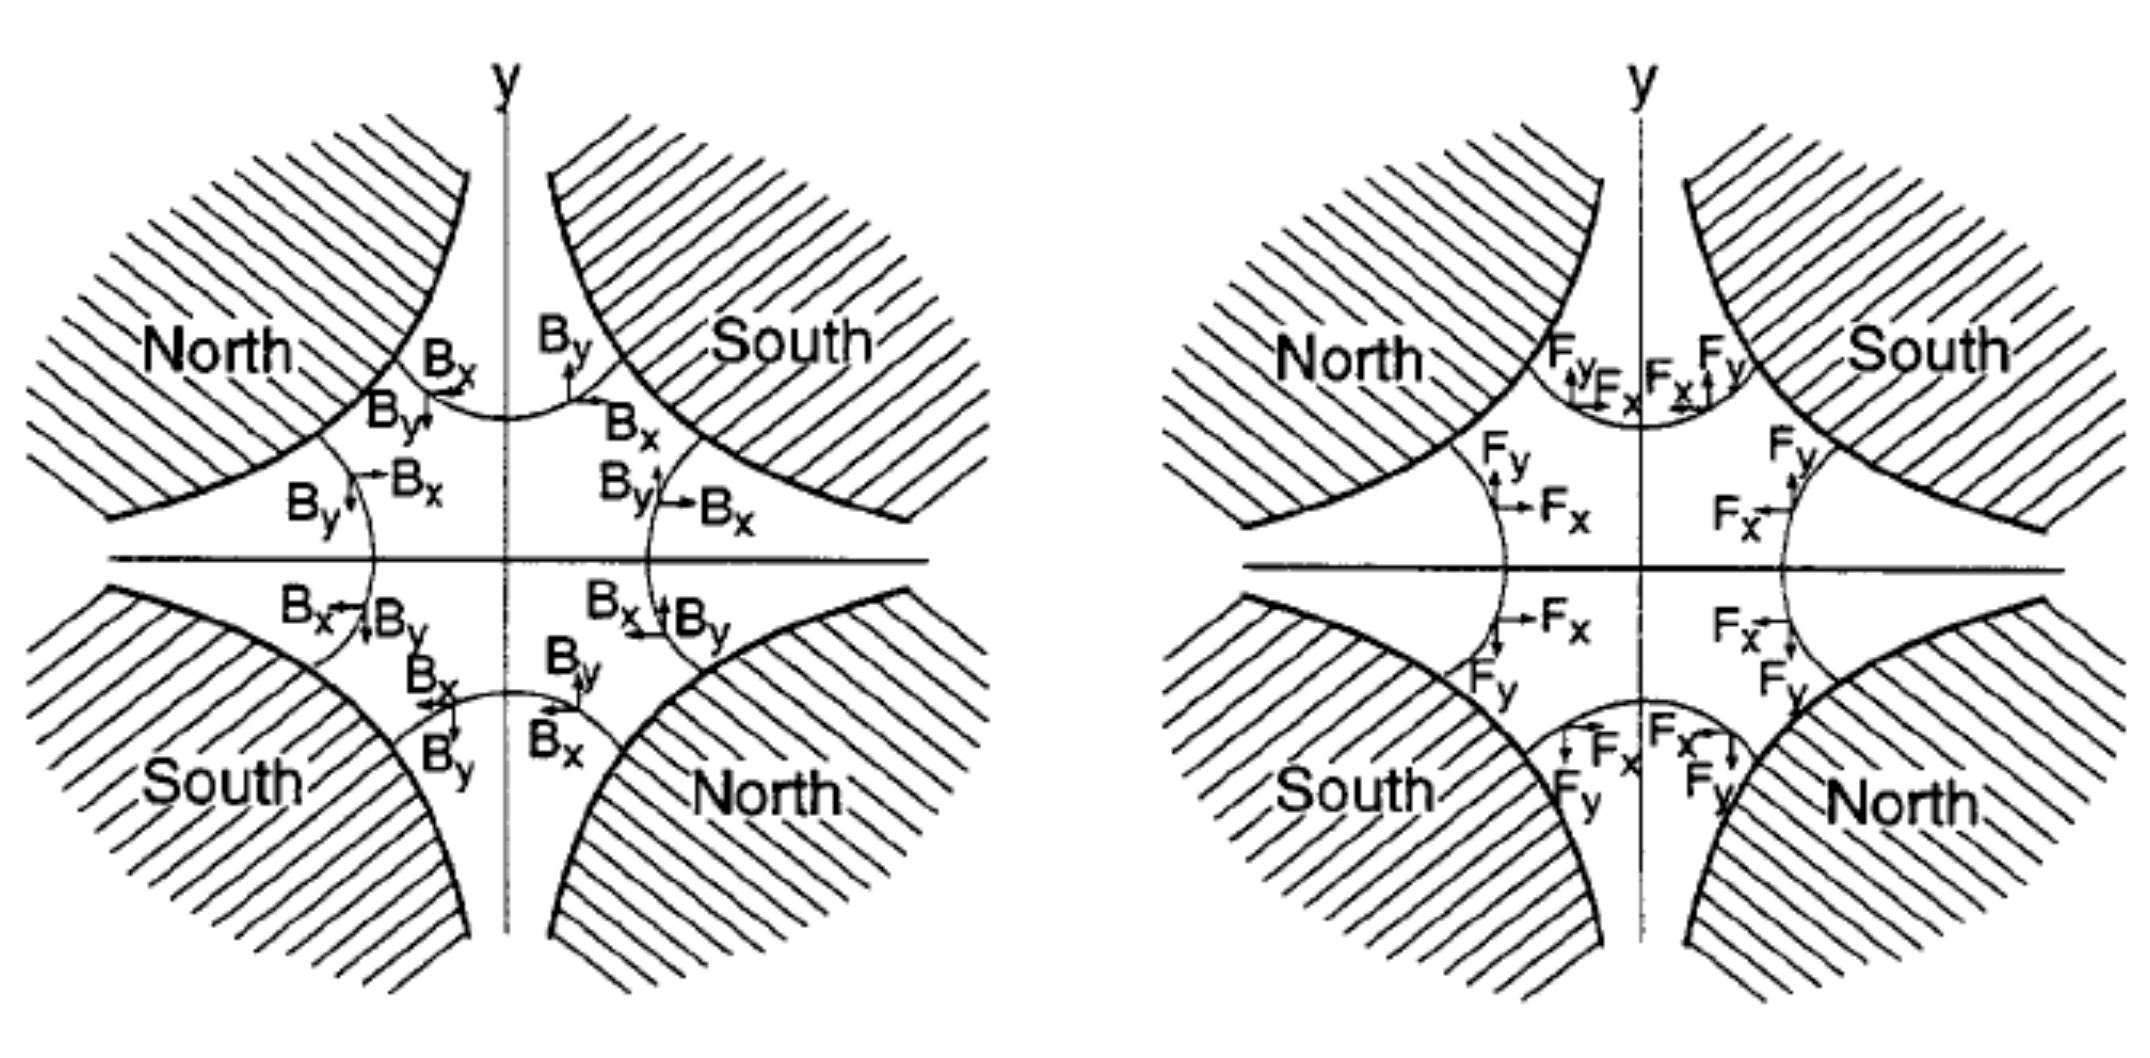
\includegraphics[width=250pt]{fig7_08}
\caption{A sinistra sono evidenziale le linee di campo del quadrupolo mentre a destra le forze generate}
\end{figure}

Le forze sono sempre ricavate utilizzando la forza
\begin{equation}
\vec{F}=q\vec{v}\times\vec{B}
\end{equation}
Tralasciando i segni abbiamo quindi che 
\begin{equation}
F_x=qvB_y\hspace{1cm} F_y=qvB_x
\end{equation}
La differenza tra la forza che agisce lungo l'asse delle $x$ e l'asse delle $y$, è che la forza $F_x$ tende a focalizzare il fascio mentre la forza $F_y$ tende a defocalizzarlo nel senso che una avvicina al centro mentre l'altra allontana.
Abbiamo inoltre che i campi in questo caso particolare tendono ad aumentare e quindi a generare più forza più ci si allontana dal centro di coordinate, corrispondente al centro del quadrupolo.
\begin{equation}
\begin{split}
B_y & \propto x\\
B_y & =\frac{dB_y}{dx}x\\
F_x & =qvB_y=qv\frac{dB_y}{dx}x
\end{split}
\end{equation}

L'effetto di questa forza è quello di variare la quantità di moto.
\begin{equation}
\Delta p_x=F_x \Delta t=qv\frac{dB_y}{dx}x \frac{d}{v}=q\frac{dB_y}{dx}xd
\end{equation}
dove $d$ è la profondità del magnete.
Si ha quindi che la variazione della quantità di moto è linearmente dipendente dalla posizione della particella.
L'effetto di una variazione della quantità di moto è di variare la pendenza della particella lungo l'asse delle $x$.
\begin{equation}
\Delta x'=\frac{\Delta p_x}{p}=qx \frac{B_y}{dx}\frac{d}{p}
\end{equation}
Si ha dunque che 
\begin{equation}
\Delta x' \propto x
\end{equation}
L'effetto di un quadrupolo magnetico in definitiva è quello di variare l'inclinazione di una particella rispetto all'asse $z$ in funzione della sua distanza dal centro il che corrisponde esattamente all'effetto di una lente che focalizza ad una distanza 
\begin{equation}
f=-\frac{p}{\frac{dB_y}{dx}d}
\end{equation}
(il segno meno indica l'effetto di focalizzazione).

Come si è già visto se una componente focalizza l'altra defocalizza e il punto focale sarà 
\begin{equation}
f=+\frac{p}{\frac{dB_x}{dy}d}
\end{equation}
La peculiarità dei quadrupoli magnetici è che focalizzando in una direzione si va a defocalizzare nell'altra.
Per avere la focalizzazione si dovrà allora sfruttare quello che in ottica viene chiamato doppietto, ovvero il sistema composto da due lenti con lunghezze focali $f_1, f_2$ poste ad una distanza $d$.
In questo modo la focale equivalente è 
\begin{equation}
\frac{1}{f}=\frac{1}{f_1}+\frac{1}{f_2}-\frac{d}{f_1f_2}
\end{equation}
Che nel nostro caso può essere semplificato a 
\begin{equation}
f_1=-f_2\to \frac{1}{f}=\frac{d}{f_1f_2}
\end{equation}

Per descrivere matematicamente questo sistema si sfrutta un formalismo matriciale ovvero si va a schematizzare ogni elemento con una matrice che prende un valore di ingresso e me lo restituisce trasformato.
\begin{equation}
\begin{pmatrix}
u\\
u'
\end{pmatrix}_{out}
=
\begin{pmatrix}
C & S\\
C' & S'
\end{pmatrix}
\begin{pmatrix}
u\\
u'
\end{pmatrix}_{in}
\end{equation}
Vuol dire che io prendo qualunque elemento e riassumo il suo  effetto in quello di trasformare una serie di condizioni del fascio in ingresso nelle condizioni del fascio in uscita.
Nel caso generale mettendo insieme $x$ e $y$ avremo delle matrici $4\times 4$ che moltiplicano dei vettori che ci indicano le posizioni radiali del fascio.
\begin{equation}
\begin{pmatrix}
x\\x'\\y\\y'
\end{pmatrix}_{out}
=
\begin{pmatrix}
C_x&S_x&0&0\\C'_x&S'_x&0&0\\0&0&C_y&S_y\\0&0&C'_y&S'_y
\end{pmatrix}
\begin{pmatrix}
x\\x'\\y\\y'
\end{pmatrix}_{in}
\end{equation}
Tutte queste sono funzioni del tipo
\begin{equation}
x=x(s)
\end{equation}
Dove $s$ mi indica la posizione dell'elemento lungo l'anello.
Gli $0$ nelle matrici mi indicano che gli elementi non perturbano.

Per esempio si prenda una particella in posizione $x_0$ in movimento, costruiamone la \emph{matrice di drift}.
\begin{figure}
\centering
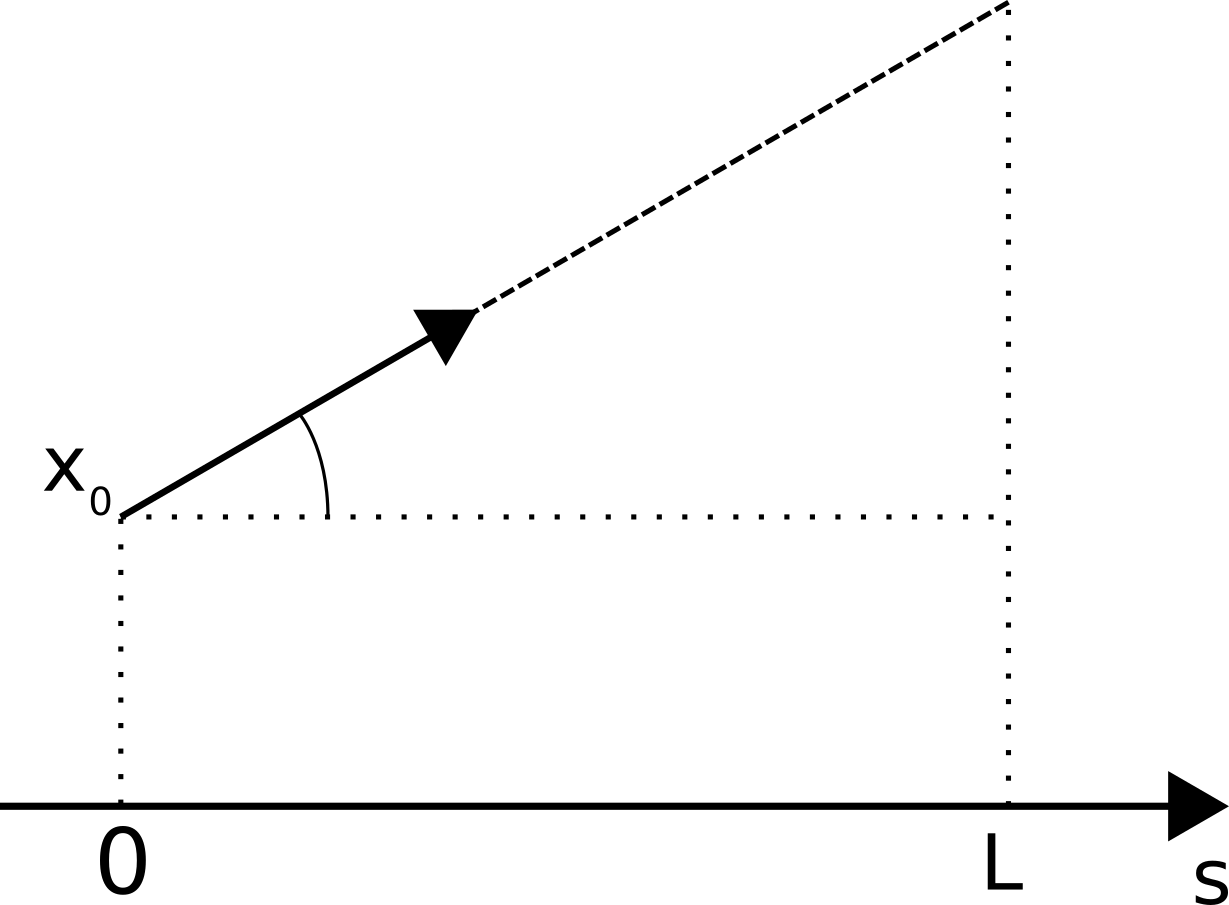
\includegraphics[width=150pt]{fig7_09}
\end{figure}

Quello che si otterrà dopo una distanza $L$ dovrebbe essere uno spostamento del tipo
\begin{equation}
\begin{split}
x(L) & =x_0+Lx'_0\\
x'(L) & =x'_0
\end{split}
\end{equation}
in quanto la particella è soggetta ad una forza che la muove verso l'alto.
La situazione viene descritta in forma matriciale
\begin{equation}
\begin{pmatrix}
x\\x'
\end{pmatrix}_{out}
=
\begin{pmatrix}
1&L\\0&1
\end{pmatrix}
\begin{pmatrix}
x\\x'
\end{pmatrix}_{in}
\end{equation}

La rappresentazione di un quadrupolo deve esprimere la variazione della pendenza.
Quello che si vede nel caso di una lente focalizzante è che 
\begin{equation}
x{out}=x_{in}\hspace{1cm}x'_{out}=-\frac{1}{f}x_{in}+x'_{in}
\end{equation}
che in forma matriciale diventa
\begin{equation}
\begin{pmatrix}
x\\x'
\end{pmatrix}_{out}
=\begin{pmatrix}
1&0\\-\frac{1}{f}&1
\end{pmatrix}
\begin{pmatrix}
x\\x'
\end{pmatrix}_{in}
\end{equation}
Nel caso della lente defocalizzante si avrà invece
\begin{equation}
\begin{pmatrix}
y\\y'
\end{pmatrix}_{out}
=\begin{pmatrix}
1&0\\+\frac{1}{f}&1
\end{pmatrix}
\begin{pmatrix}
y\\y'
\end{pmatrix}_{in}
\end{equation}

Per completezza mostriamo anche la matrice rappresentante un dipolo
\begin{equation}
\begin{pmatrix}
x\\x'
\end{pmatrix}_{out}
=\begin{pmatrix}
\cos\theta & \sin\theta \\-\frac{1}{\rho}\sin\theta & \cos\theta
\end{pmatrix}
\begin{pmatrix}
x\\x'
\end{pmatrix}_{in}
\end{equation}
dove $\rho$ rappresenta il raggio di curvatura.


\section{Diffusione elettronica per studi subnucleari}

\section{Il Modello Standard}
In questa sezione verrà studiato quello che è il modello standard delle particelle, ovvero tutte le leggi date per confermate e che costituiscono la base degli studi fisici. 
Esistono delle teorie con evidenze sperimentali che vanno oltre a questo modello ma sono spesso teorie non ancora totalmente sviluppate che verranno implementate.
Lo studio del modello standard sarà approfondito nei corsi della magistrale ma è giusto che uno studente della triennale abbia comunque un'idea generale di quello che è.

%nuova sezione------------------------------------------------------------------------------ 
\subsection{Fisica degli acceleratori di particelle}
La conoscenza della fisica degli acceleratori è essenziale per ogni tipo di fisico in quanto ha applicazioni in ogni campo fisico.
Ne approfondiamo quindi quelli che sono i fondamenti e le grandezze base per poter avere un'idea più chiara del loro funzionamento.

Per capire la grande applicabilità di questi strumenti, attualmente al mondo sono attivi $15000$ acceleratori di cui: $8500$ con applicazioni industriali, $5500$ con applicazioni mediche e $1000$ con applicazioni in ricerca (di cui $100$ usati per la fisica nucleare e subnucleare).
L'attenzione mondiale alla fisica nucleare cambiò radicalmente prima e dopo la seconda guerra mondiale e anche gli acceleratori sono figli dell'aumento dell'interesse a questi ambiti.
Già a Rutherford dopo i suoi studi era chiaro che l'accelerazione di particelle sarebbe stato il passo successivo per la scoperta e l'approfondimento di questa nuova fisica.
Solo avendo il controllo della quantità ed energia di particelle si sarebbe potuto infatti ottenere una maggiore risoluzione nello studio del nucleo.

I parametri che caratterizzano gli acceleratori sono sostanzialmente l'energia e la luminosità.

\paragraph{Energia}. 

\'E importante conoscere l'energia perché la risoluzione con la quale possiamo risolvere un bersaglio dipende dalla lunghezza d'onda della sonda con la quale bombardiamo l'oggetto in analisi.
Prendendo un oggetto di raggio R, la lunghezza d'onda della sonda dovrà essere
\begin{equation}
\begin{split}
\lambda=\frac{h}{p}&<2R\\
2\pi \frac{\hbar c}{pc}&<2R
\end{split}
\end{equation}
Vuol dire che se vogliamo risolvere una struttura di dimensione $2R$ dobbiamo avere un fascio di energia
\begin{equation}
pc\simeq E>2\pi\frac{\hbar c}{2R}
\end{equation}
Inserendo quindi un po' di dimensioni, se vogliamo per esempio studiare il protone ($r=1fm$) serve un energia pari a 
\begin{equation}
E=pc=600MeV
\end{equation}
Se per esempio invece volessimo studiare i quark($r=10^{-4}fm$) allora l'energia sarà
\begin{equation}
E\simeq 6TeV
\end{equation}

Un altro motivo per cui è essenziale l'energia negli acceleratori deriva dalla famosa formula di Einstein
\begin{equation}
E=mc^2
\end{equation}
Che prevede la convertibilità tra massa ed energia.
Nella sezione precedente abbiamo infatti visto come sia possibile generare energia trasformando della massa.
Se questo è vero allora sarà vero anche il contrario, infatti è stato visto negli acceleratori che da scontri tra particelle altamente energetiche è possibile generare nuove particelle.
Per cui un grande utilizzo di questi apparati deriva proprio dalla necessità di generare particelle che sono state crucciali nello studio dell'evoluzione dell'universo che però sono ormai decadute per il basso tempo di decadimento.
Per dire proprio a questo scopo è stato costruito l'LHCb del Cern.

\paragraph{Metodi di collisione}
Esistono due modi per studiare le collisioni tra particelle: il metodo con il collisore e la collisione su bersaglio fisso.
Nel caso di collider (metodo del collisore) si sfruttano due fasci il che porta a delle energie nel centro di massa molto elevate (è quindi adatto alla produzione di nuove particelle).
Nel caso invece del bersaglio fisso l'energia è più bassa, ergo si fa più fatica a produrre nuove particelle, è favorita però la \emph{luminosità}.

Facciamo quindi delle stime sui due metodi
\begin{itemize}
\item Caso del collisore simmetrico.

Si consideri di avere due fasci paralleli e opposti in collisione, per semplicità adotteremo la semplificazione $\hbar=c=1$.
Il quadrivettore legato alla particella 1 è dato da
\begin{equation}
p_1*=(E_1*,\bar{p})
\end{equation}
(con asterisco indico le quantità misurate nel centro di massa).
Siccome i due fasci hanno lo stesso momento contropropagante è utile porsi nel sistema di riferimento del centro di massa , inoltre le due quantità di moto saranno identiche per cui non serve distinguere tra $\bar{p_1}$ e $\bar{p_2}$.
\begin{equation}
p_2*=(E_2*,-\bar{p})
\end{equation}
Si sa dalla meccanica relativistica che il quadrato del quadrivettore è un invariante relativistico
\begin{equation}
{p_1*}^2=E_1*-\bar{p}^2=m_1^2\\hspace{0.5cm}{p_2*}^2=E_2*-\bar{p}^2=m_2^2
\end{equation}
L'energia nel centro di massa è la somma dei quadrivettori al quadrato
\begin{equation}
\begin{split}
&s=(p_1*+p_2*)2=(E_1*+E_2*, \bar{p}-\bar{p})^2\\
&\to E_{CM}=\sqrt{s}=E_1*+E_2*
\end{split}
\end{equation}
Suppongo che il collider è simmetrico e che le particelle scontrate siano in entrambi i casi protoni (quindi di massa $m_p$).
L'energia di ogni fascio sarà
\begin{equation}
E_1*=m_1+T_{cm}=m_p+T_{cm}
\end{equation}
L'energia invece del centro di massa corrisponde a 
\begin{equation}
\sqrt{s}=E_{cm}=2m_p+2T_{cm}
\end{equation}
Quello che ci interessa è che se suppongo che l'energia nel centro di massa sia molto maggiore della massa del protone ($T_{cm}\gg m_p$), ottengo
\begin{equation}
T_{cm}=\frac{\sqrt{s}}{2}\to \sqrt{s}=2T_{cm}
\end{equation}
Quello che ci interessa è che in un collider l'energia nel centro di massa è linearmente dipendente dall'energia cinetica nel centro di massa.
Questo è importante perché quello che voglio creare nel centro di massa sono nuove particelle e così posso controllarne l'energia.

Il collider è un concetto molto complicato in quanto non è banale far scontrare due fasci, bisogna considerare che le dimensioni dei fasci infatti sono dell'ordine del millimetro e l'acceleratore è spesso lungo centinaia di metri.

Supponiamo di far scontrare due protoni e di voler creare un pione, particella costituita da un quark ed un anti quark.
\begin{equation}
pp\to pp\pi^0
\end{equation}
La massa di un pione è di 
\begin{equation}
m_{\pi^0}\simeq 130MeV/c^2
\end{equation}
L'energia dei due fasci per la formazione di un pione deve essere uguale a 
\begin{equation}
s_{cm}=(2m_pmm_{\pi^0})^2
\end{equation}
L'energia cinetica delle particelle deve soddisfare la condizione
\begin{equation}
2m_p+2T_{cm}\ge 2m_p+m_{\pi^0}
\end{equation}
e quindi essere
\begin{equation}
T_{cm}\ge \frac{m_{\pi^0}}{2}=67,5MeV
\end{equation}
L'energia cinetica richiesta per ogni fascio sarà quindi sempre pari alla metà dell'energia di massa della singola particella.
Questo si ottiene in quanto dobbiamo considerare che il centro di massa sarà sempre uguale.

\item Caso del bersaglio fisso.

Nel sistema di riferimento del laboratorio abbiamo che i due quadrivettori saranno 
\begin{equation}
\begin{split}
p_1&=(E_1,\bar{p_1}\\
p_2&=(m_2,0)
\end{split}
\end{equation}
Nel centro di massa il quadrivettore energia è 
\begin{equation}
\begin{split}
s&=[(E_1+m_2)^2-(\bar{p_2}+0)^2]\\
&=E_1^2+2E_1m_2+m_2^2-\bar{p_1}^2\\
&=m_1^2-+m_2^2+2E_1m_2
\end{split}
\end{equation}
A questo punto faccio le stesse considerazioni del collider, suppongo che le due particelle coincidano ($m_1=m_2=m_p$) e che l'energia della prima particella sia
\begin{equation}
E_1=m_1+T^{lab}
\end{equation}
ottengo quindi 
\begin{equation}
\begin{split}
s & =m_p^2 + m_p^2 + 2(m_p+T^{lab})m_p\\
\sqrt{s}&=\sqrt{4m_p^2+2T^{lab}m_p}
\end{split}
\end{equation}
Se mi pongo nella condizione in cui $T^{lab}\gg m_p$ ottengo
\begin{equation}
\sqrt{s}=\sqrt{2m_pT^{lab}}
\end{equation}

La differenza con il caso precedente è immediata, in un esperimento a bersaglio fisso l'energia nel centro di massa cresce linearmente con $\sqrt{T^{lab}}$.
Se volessi creare un pione con questa configurazione dovrei richiedere un'energia di soglia
\begin{equation}
\begin{split}
T^{lab}_{Th}&=\frac{s_{Th}-4m_p^2}{2m_p}\\
s_{Th}&=(2m_p+2m_{\pi^0})^2\\
T^{lab}_{Th}&=\frac{(2m_p+2m_{\pi^0})^2-4m_p^2}{2m_p}=280MeV
\end{split}
\end{equation}
Questo è solo un esempio per capire la differenza tra i due tipi di acceleratore.
\end{itemize}

\paragraph{Luminosità}
La luminosità $L$ corrisponde al numero di eventi (collisioni) per unità di area al secondo, è una grandezza importante perché se voglio calcolare il rate di eventi di un certo tipo 
\begin{equation}
R=\sigma L
\end{equation}
dove $\sigma$ è la sezione d'urto.

Per esempio nel Lep, che è stata la macchina progenitrice dell'LHC (funzionante tramite leptoni) e con cui si è studiato il modello standard, la produzione di coppie $W^+, W^-$ era di $\sigma=15pb$ e la luminosità (che si misura in numero di particelle su centimetro quadro al secondo) era di $L=10^{32}\cdot/cm^2s$.
Il che restituiva un rate di coppie pari a 
\begin{equation}
\frac{dW^+W^-}{dt}=15\times 10^{-12}\times 10^{-28}m^2\cdot 10^{32}\frac{1}{cm^2s}=1,5\times 10^{-3}\frac{eventi}{s}
\end{equation}
Si verificavano quindi un paio di eventi ogni ora.

La luminosità integrata nel tempo è una quantità che serve per capire per quanto tempo ho la necessità di sfruttare una strumentazione
\begin{equation}
L=\int Ldt
\end{equation}

La luminosità nel caso del collider si calcola come
\begin{equation}
L=\frac{nfN_1N_2}{A}
\end{equation}
dove $n$ è il numero di bunches (le particelle solitamente non sono distribuite uniformemente nei fasci a causa dei metodi sfruttati per collimare i fasci, vengono invece distribuite in pacchetti), $N_1, N_2$ sono il numero di particelle per bunch (ce ne sono due perché abbiamo due fasci e non sempre sono fasci uguali), $f$ è la frequenza di rivoluzione e $A$ è la sezione del fascio.
\'E intuitivo che per aumentare la luminosità dobbiamo rendere il fascio più piccolo possibile.

Nel caso del bersaglio fisso la luminosità è data da
\begin{equation}
L=\Phi_a N_b
\end{equation}
dove $\Phi_a$ è l'intensità di particelle del fascio e $N_b$ è il numero di particelle nel bersaglio.
L'intensità di particelle del fascio è uguale al numero di particelle al secondo diviso l'area
\begin{equation}
\Phi_a=\frac{N_a(s)}{A}
\end{equation}
che può anche essere scritta come la densità di particelle per unità di volume per la velocità delle particelle stesse
\begin{equation}
L=n_a v_a
\end{equation}
Mentre il numero di particelle del bersaglio è uguale alla densità delle particelle del bersaglio per lo spessore per l'area interessata del fascio
\begin{equation}
N_b=n_bd\cdot A
\end{equation}
La luminosità è quindi riscrivibile come
\begin{equation}
L=N_an_bd=n_av_aN_b
\end{equation}

%nuova sezione-----------------------------------------------------------------------------
\subsection{Tipi di Acceleratore}
Gli acceleratori si possono suddividere in due grandi categorie: acceleratori lineari e circolari.
\paragraph{Acceleratori Lineari}
Sono acceleratori elettrostatici ossia in questi acceleratori l'accelerazione avviene tramite una differenza di potenziale elettrostatico. 
In questa categoria sono inclusi gli acceleratori: 
\begin{itemize}
\item Van de Graaf
\item Cockrof-Walton
\item Tandem
\item il LINAC.
\end{itemize}
Il limite di questi acceleratori sta nel fatto che utilizzano un'unica differenza di potenziale, il che pone un limite a ciò che si può creare infatti le differenze di potenziale sono limitate dalla rottura del dielettrico.
Sono i primi che sono stati utilizzati e i massimi campi che si riesce a creare nel vuoto sono di $6-7MeV/m$

\paragraph{Acceleratori circolari}
Questi acceleratori ovviano al limite della differenza di potenziale facendo passare la particella più volte per la stessa differenza di potenziale facendo bastare così una piccola differenza di potenziale ben posta.
Di questi fanno parte:
\begin{itemize}
\item ciclotrone
\item betatrone
\item sincrotrone
\end{itemize}

\paragraph{Van De Graaf}
\begin{figure}[h]
\centering 
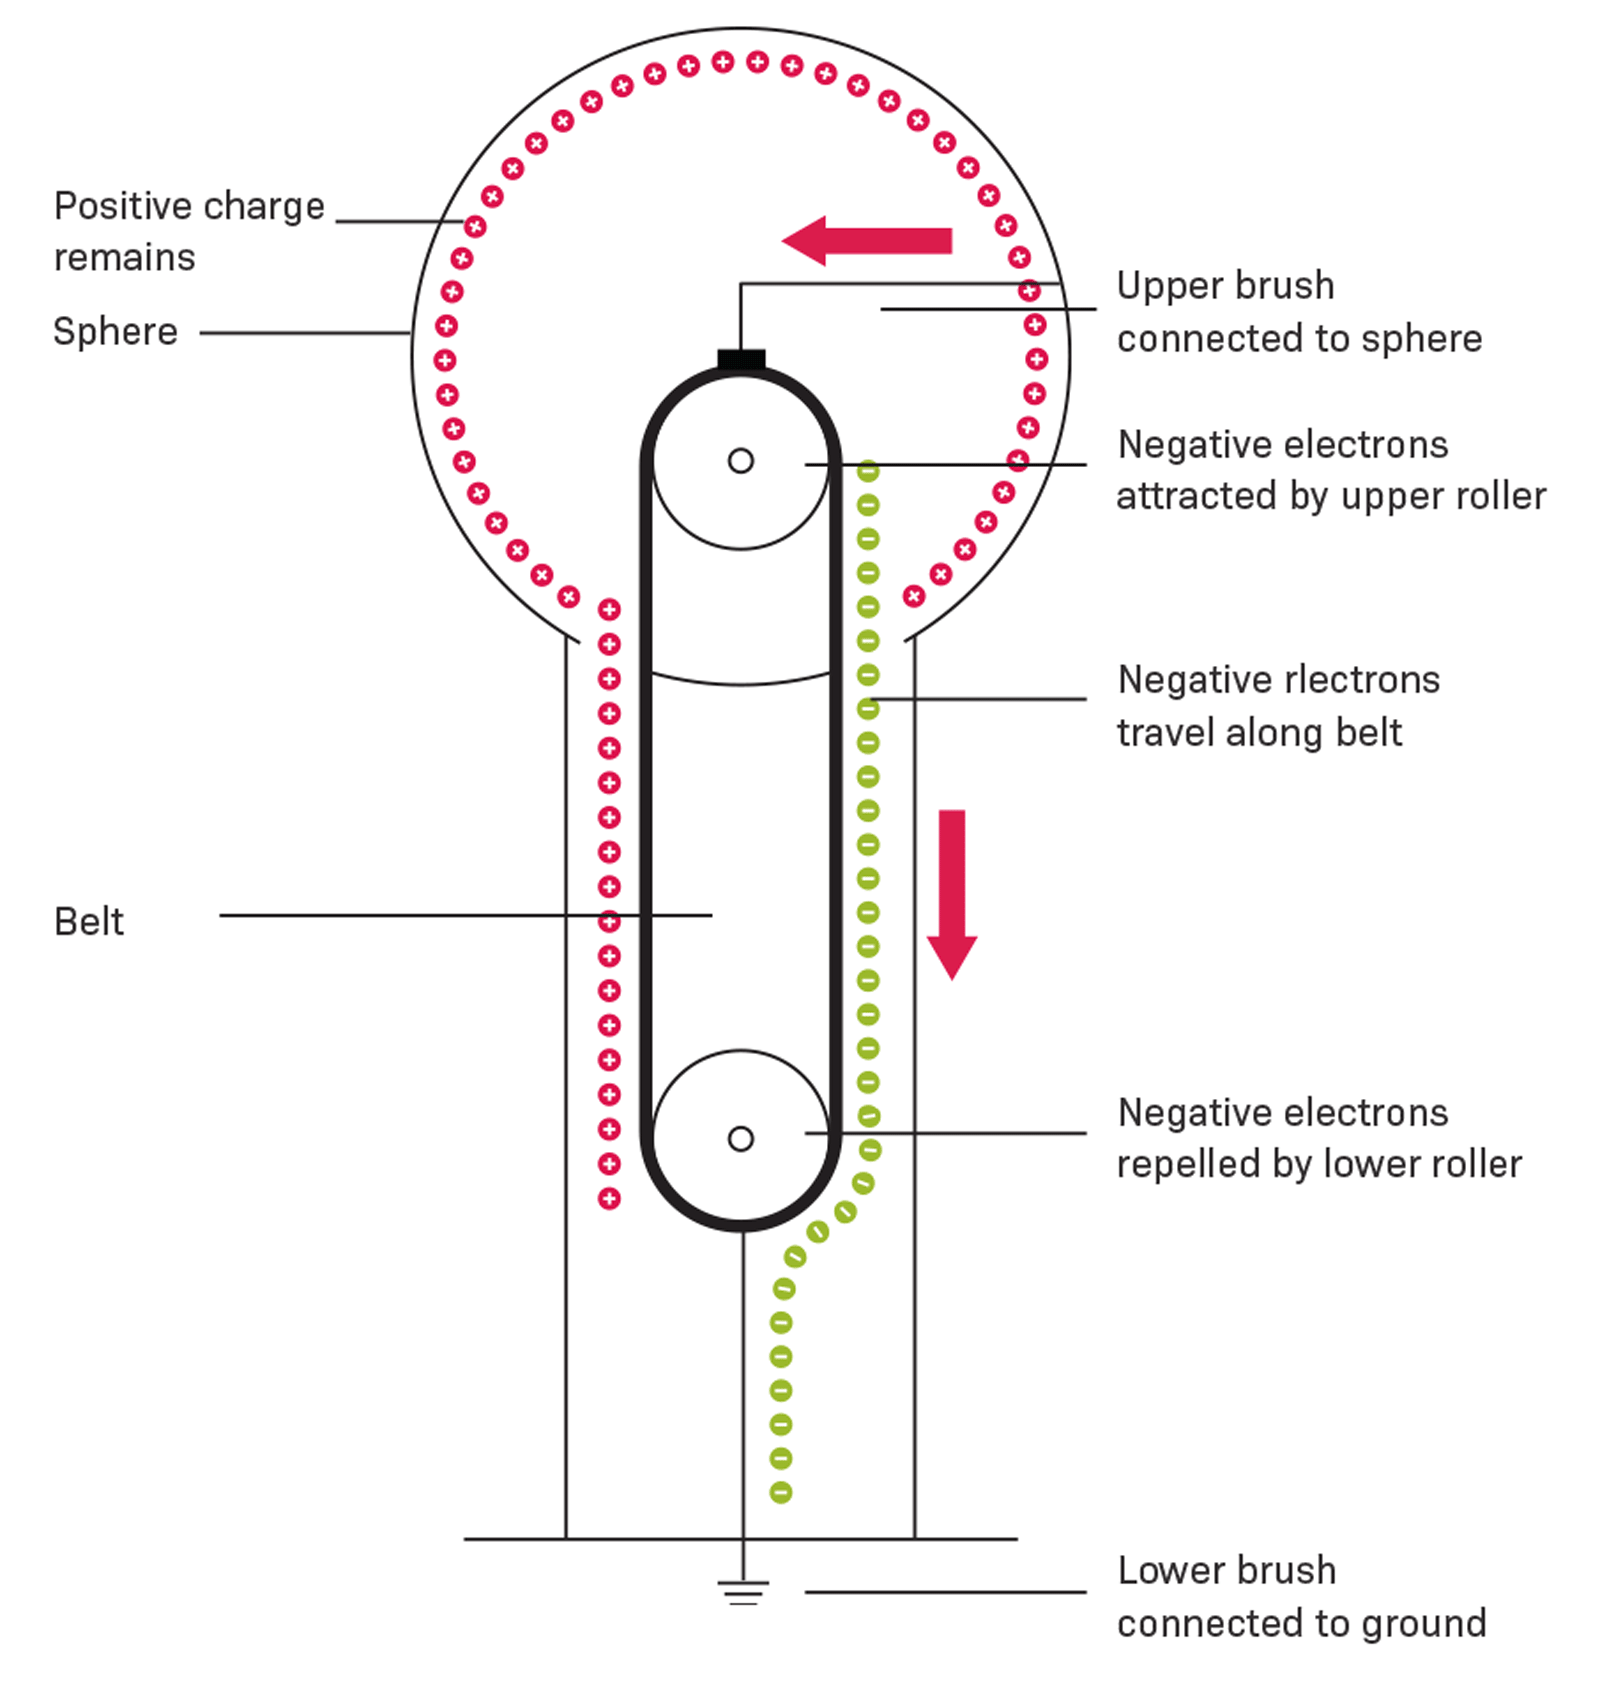
\includegraphics[width=160pt]{fig7_01}
\caption{Schema di un acceleratore di van de Graaf}
\end{figure}
L'acceleratore di Van De Graaf si compone come in figura.
La struttura è formata da una cinghia che scorre e si carica grazie a delle punte per scorrimento.
La cinghia poi passa per una sfera cava su cui viene trasferita la carica che, per i principi dell'elettrodinamica, si va a distribuire su tuttala superficie.
In questo modo si riescono a creare una differenza di potenziale dell'ordine di qualche $MeV$.
Tutto il sistema viene messo all'interno di grossi contenitori isolati in quanto l'aria farebbe scaricare le superfici (i gas inerti sostitutivi sono solitamente $SF_6, N_2+CO_2$).

Il \textbf{Tandem}, è basato sullo stesso principio del Van de Graaf, solo che la differenza di potenziale viene raddoppiata, ponendo la sfera all'interno di un altro conduttore.
\begin{figure}[h]
\centering
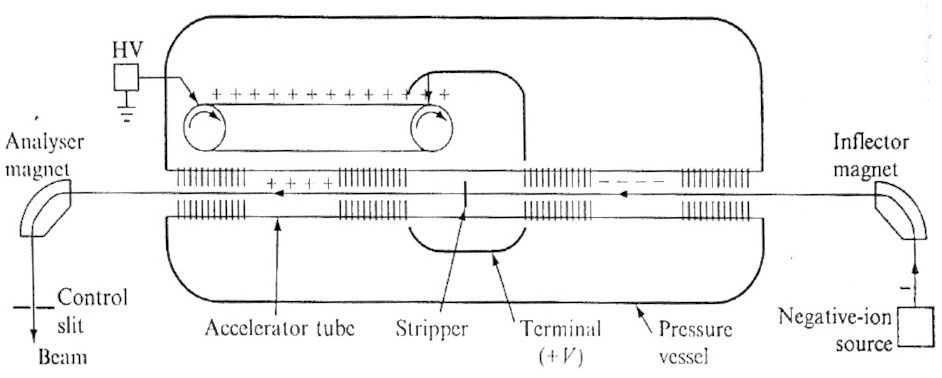
\includegraphics[width=200pt]{fig7_02}
\caption{Configurazone Tandem}
\end{figure}
Il potenziale che si riesce a creare è il doppio del potenziale di partenza.
A Legnaro è presente un acceleratore con questa configurazione e viene utilizzato per esperimenti di \emph{Rutherford backscattering}, in cui si sfrutta lo scattering del fisico neozelandese per esperimenti di spettroscopia (studiando l'energia delle particelle backscatterate si riesce a capire la composizione superficiale del bersaglio).

\paragraph{Acceleratore lineare: LINAC}
Il LINAC è stato rivoluzionario come acceleratore perché supera il limite nella generazione di potenziali.
Questo acceleratore è composto da una serie di elettrodi separati che variano la polarità con un'onda a radiofrequenza.
\begin{figure}[h]
\centering
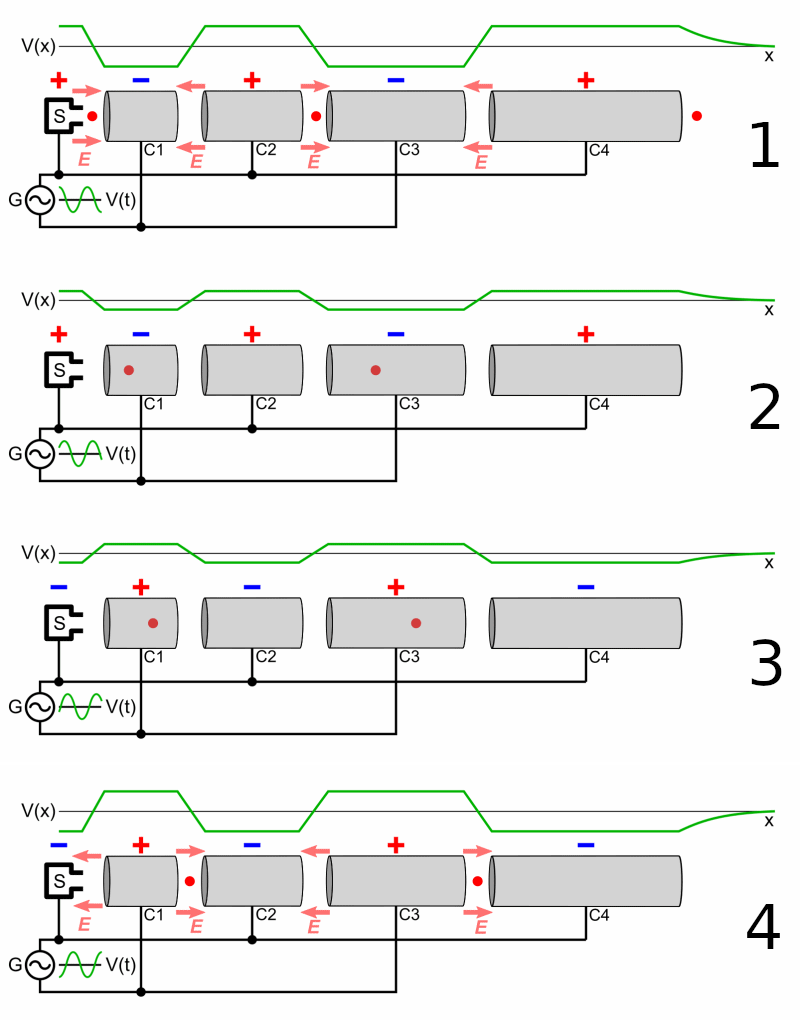
\includegraphics[width=180pt]{fig7_03}
\caption{Schema di funzionamento di un acceleratore lineare}
\end{figure}

Quello che si vuole generare con questo tipo di configurazione è un potenziale sempre negativo per la particella accelerata, infatti riuscendo a variare il potenziale al passaggio della particella, facendolo passare da positivo a negativo e viceversa, la particella nel sistema sarà sempre accelerata da un potenziale negativo rispetto a quello che ha alle sue spalle (che nel frattempo è diventato positivo).
Tutto questo fa si che pur mantenendo una differenza di potenziale piuttosto bassa si riesca ad accelerare particelle ad alte energie, questo metodo è usato per esempio per gli elettroni (in orbita circolare gli elettroni emettono radiazione).

\paragraph{Ciclotrone}
Il ciclotrone utilizza una combinazione di campi elettrici e magnetici.
Supponiamo di avere un campo magnetico entrante e di porci una particella (per esempio un protone) ciò che si crea è una forza di Lorentz, quindi a causa del campo magnetico la particella percorre una traiettoria circolare.
\begin{figure}[h]
\centering
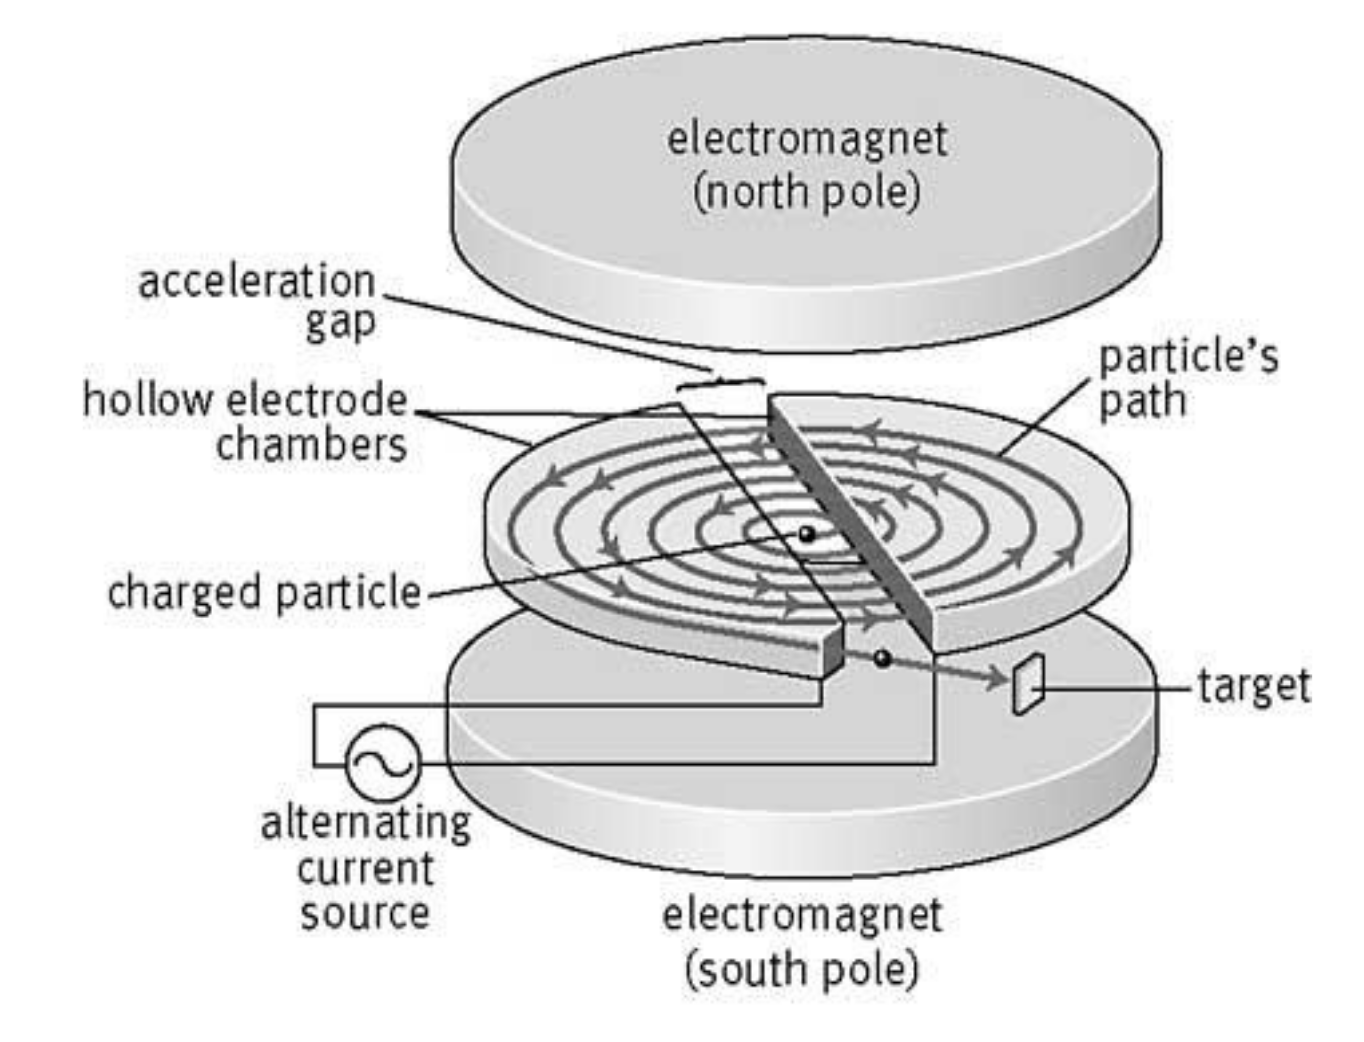
\includegraphics[width=150pt]{fig7_04}
\caption{Struttura del ciclotrone}
\end{figure}

All'interno di una situazione in cui due elettrodi hanno forma a D e sono immersi all'interno di un campo magnetico, questi vengono polarizzati uno con polarità positiva e uno con polarità negativa.
Se non si fa nulla il protone passa dal $+$ al $-$ e se cambio a polarità fa il percorso inverso.
Siccome voglio confinare la particella  applico un campo magnetico ortogonale al piano degli elettrodi.
La combinazione di campo magnetico e cambio di polarità genera un moto circolare del protone che ad ogni passaggio viene accelerato.
In questo modo si riesce ad aumentare la velocità delle particelle fino a che non raggiunge la velocità desiderata e allora posso estrarlo.

Calcoliamo le leggi che agiscono sulla particella.
Innanzitutto si ha la forza di Lorentz
\begin{equation}
F=Bqv
\end{equation}
Che corrisponde alla forza centripeta
\begin{equation}
Bqv=m\frac{v^2}{r}\to v=\frac{Bqr}{m}
\end{equation}
Calcoliamo la frequenza di variazione del campo elettrico per mantenere la particella in moto.
Il periodo di rotazione della particella è
\begin{equation}
T=\frac{2\pi r}{v}=\frac{2\pi r}{\frac{Bqr}{m}}=\frac{2\pi m}{Bq}
\end{equation}
Quindi la frequenza con cui devo variare i due elettrodi sarà
\begin{equation}
f=\frac{Bq}{2\pi m}
\end{equation}
\'E interessante notare come questa non dipenda dal raggio perché a mano a mano che la velocità aumenta la particella percorre percorsi maggiori e quindi queste due quantità si compensano.
Questo è ovviamente valido finché non si manifestano effetti relativistici sulla massa
\begin{equation}
m=m_0\cdot \gamma
\end{equation}
Esiste quindi un limite che corrisponde a qualche percentuale della velocità della luce (per esempio un protone che ha massa dell'ordine del $GeV$ può essere accelerato fino ad un massimo di $\sim 20MeV$).


%\include{sections/NUOVOCAPITOLO}

%Zarantonello Umberto 22/04/21
\section{Esercizi}
\subsection{Settimana 1}
\paragraph{Es. 1:}
Si calcoli la velocità media di:
\begin{itemize}
\item Molecole d'aria a temperatura ambiente
\item Eletroni atomo idrogeno
\item Terra attorno al sole
\item Elettroni che escono da un vecchio tubo catodico
\end{itemize}
\paragraph{Ris.:}
\begin{itemize}
\item \textbf{Molceole d'aria}
supponiamo di essere a $20^oC$ corrispondenti a $293K$ si sfrutti la teoria cinetica dei gas
\begin{equation}
\frac{3}{2}K_BT=\frac{1}{2}m<v^2>
\end{equation}
Si approssimi l'aria come azoto $N_2$ la cui massa molecolare è $M_{N_2}=28$
si ottiene
\[
\sqrt{<v^2>}=\sqrt{\frac{3K_BT}{m_{N_2}}}=\sqrt{\frac{3\times1,3\times10^{-23}293}{28\cdot 1,66\times10^{-27}kg}}=510\frac{m}{s}
\]
\item \textbf{Elettroni dell'idrogeno}
Ricordando la costante di Ridberg ovvero il potenziale di dissociazione dell'idrogeno, questa può essere considerata pari alla sua energia cinetica.
\[
E=13.5eV=K_e\\
K=135\times10\cdot1,6\times10^{-19}J=2,1\times10^{-18}J=\frac{1}{2}m_ev^2
\]
conoscendo la massa dell'elettrone corrispondente a $m_e=9,1\times10^{-31}kg$ si ottiene che la velocità dell'elettrone sarà
\[
v_e=\sqrt{\frac{2K_e}{m_e}}=2,1\times10^6\frac{m}{s}
\]
Si può notare che questa è una conferma che l'elettrone sia una particella non relativistica.
\end{itemize}
Si lasciano al lettore gli altri due punti.

\paragraph{Es. 2:}
Si calcoli il numero di molecole nell'atmosfera.
\paragraph{Ris.:}
Si parte considerando la massa dell'atmosfera, che si può calcolare partendo dalla pressione atmosferica, corrispondente al dell'aria sopra un metro quadro.
\[
p=10^5\frac{N}{m^2}\longrightarrow M=10^4\frac{kg}{m^2}
\]
Si consideri, ora la superficie della terra 
\[
A_{terra}=4\pi R^2=12(6\times10^6m)^4=4\times10^14m^2
\]
Si può quindi trovare la massa dell'aria
\[
M_{aria}=10^4\frac{kg}{m^2}4\times10^{14}m^2=4\times10^{18}kg
\]
Per calcolare il numero di molecoe di aria, si consideri il pero molecolare di azoto e ossigeno
\[
N_2=28\hspace{0,5cm}O_2=32
\]
Il che in media corrisponde ad un peso molecolare di $30$.
Una mole peserà dunque $30g$
\[
M_{aria}=\frac{4\times10^21g}{30g/mol}=1,3\times10^{20}mol
\]
Il numero di molecole d'aria corrispondera quindi alla massa in moli dell'aria moltiplicata per il numero di Avogadro $N_A=6\times10^{23}$
\[
N_{aria}=M_{aria}\times N_A\simeq 10^41molecole
\]
Se si volesse poi sapere quante molecole di aria dell'ultimo respiro di Carlo Magno sono contenute nei nostri polmoni, si dovrebbe fare il rapporto fra la quantità di aria contenuta nei nostri polmoni e quella contenuta nell'atmosfera.
\[
1mole (STP)=20L
\]
Una mole in condizioni standard corrisponde a 20 litri, la densità dell'aria corrisponderà quindi a 
\[
30\frac{g}{mol}:20\frac{L}{mol}=1,5\frac{g}{L}\\
1L\sim 1g\sim 3\times 10^{22}molecole
\]
Qual è la frazione di molecole che noi respiriamo ad ogni respiro?
La massa dell'aria totale è pari a $4\times 10^21g$ e ogni respiro corrsponde ad un peso di circa $1g$, il che restituisce un rapporto di
\[
0,25\times 10^{-21}
\]

\paragraph{Es. 3:}
si calcoli l'energia contenuta in un $kg$ di benzina, pprossimando la benzina come $CH_2$.
\paragraph{Ris.:}
Si può stimare che per ogni legame chimico l'energia sia pari a $E=1,5eV$ (\'E una stima molto approssimata).
Si considerino le masse atomiche:

Il carbonio ha massa atomica $C=12$, mentre l'idrogeno $H=1$, il che riconduce ad una massa totale pari a $CH_2=14$.

In un $Kg$ di benzina si ha
\[
N_{moli} =\frac{1Kg}{1,4\times 10^{-2}Kg/mol}=70mol
\]
Per ogni molecola di $CH_2$ avrò due reazioni
\[
C+O_2\longrightarrow CO_2\\
H_2+O\longrightarrow H_2O
\]
Corrispondente ad un'energia totale rilasciata di $3eV$.

Qual'è la densità energetica della benzina?
\[
D=70\frac{mol}{Kg}\cdot 6\times 10^{23}\frac{reazioni}{mol}\frac{3eV}{mol}\cdot \frac{1}{1,6\times 10^{-19}eV/J}=2\times 10^7\frac{J}{Kg}
\]
Questo valore è approssimativo ma si discosta solamente di un fattore 2 dal valore reale, il che ci f intuire che comunque si tratta di un buon calcolo (che il bravo fisico deve essere in grado di effettuare).

Qual è poi la potenza trasferita in un pieno?

Supponiamo che un serbatoio di un'auto di $80L$. La densità della benzina è più bassa di quella dell'acqua. 
La densità di energia per litro corrisponde a $3\times10^7\J/L$
\[
80L\cdot 3\times10^7\frac{J}{L}=2\times10^9J
\]
In 3 minuti (tempo di un pieno) l'energia trasferita corrisponde a 
\[
P=\frac{E}{\Delta t}=\frac{2\times10^9J}{180s}=10MW
\]
Impressionante!



% ------------------------------------------------
% %% commento iniziale
%% anche su più righe ma vicine


% ogni file = un capitolo 

\section{Convenzioni LaTex} %inizia il capitolo con "section"
Iniziare a scrivere subito sotto al comando section per dare un senso estetico al codice.
Andare a capo ad ogni "punto", ogni frase inizia una nuova riga di codice.
Lasciando uno spazio bianco (due volte "invio") si ottiene un nuovo inizio paragrafo.

Tipo questo, che non sempre è bello da vedere mentre altre volte è molto utile.
Il concetto è: scrivere il codice il più attaccato possibile ma con maggior leggibilità possibile.

Le equazioni si possono scrivere in vari modi, ma i migliori, per compatibilità tra versioni sono:
\begin{enumerate}
\item equazione nel testo tipo $\cos \alpha = \frac{\pi}{2 \pi}$

\item equazione a capo a centro pagina e su una riga, senza numero di equazione
$$ \frac{d\sigma}{d\Omega}=\frac{b(\theta)}{\sin\theta}\frac{db}{d\theta} $$

\item equazione a capo a centro pagina e su una riga, con numero di equazione 
\begin{equation}
\Delta p_x \Delta x \ge \frac{\hbar}{2}
\end{equation}

\item equazione a capo a centro pagina su più righe, con numero di equazione
\begin{equation}
\begin{split}
\mbox{\underline{Maxwell-Boltzmann}}  \quad\quad  \frac{n_s}{g_s} & = \frac{1}{e^{\alpha + \beta E_s}} \\
\mbox{\underline{Bose-Einstein}}  \quad\quad  \frac{n_s}{g_s} & = \frac{1}{e^{\alpha + \beta E_s} - 1} \\
\mbox{\underline{Fermi-Dirac}}  \quad\quad  \frac{n_s}{g_s} & = \frac{1}{e^{\alpha + \beta E_s} + 1 } 
\end{split}
\end{equation}

\end{enumerate}



\end{document}



